% Ensure that you compile using XeLaTeX !!! PDFTex has problems with some of the packages used
\documentclass[12pt]{article}
\setlength\parindent{0pt}

\usepackage{parskip}
\usepackage[margin=0.5in]{geometry}
\usepackage{fullpage}
\usepackage{moresize}
\usepackage{graphicx}
\usepackage{caption}
\usepackage{subcaption}
\usepackage{float}
\usepackage{xcolor}
\usepackage{soul}
\usepackage{fontspec}
\setmainfont{Doulos SIL}

\begin{document}

\begin{center}
\textbf{{\color{violet}{\HUGE 20201029 Thursday\\}}}

\textbf{{\color{violet}{\HUGE ALL EXAMS\\}}}

\end{center}
\newpage

\begin{center}
\textbf{{\color{blue}{\HUGE START OF EXAM\\}}}

\textbf{{\color{blue}{\HUGE Student ID: 10699\\}}}

\textbf{{\color{blue}{\HUGE \\}}}

\end{center}
\newpage

{\large Question 1}\\

Topic: Transcription\\
Source: Week 2 Handout, Part II\\

Is this a reasonable transcription of this word? Explain why.\\

<health>: {[hɛlð]}


\newpage

{\large Question 2}\\

Topic: Articulatory Phonetics\\
Source: Week 3 Handout, Question 7\\

Is the symbol given a reasonable way to transcribe any of the sounds described below? If so, which one? If not, why not? Explain your answer.\\

{[ʃ]}

\begin{itemize} \item voiceless palatal affricate \item voiced velar nasal \item voiceless glottal fricative \item voiced labiodental fricative \item voiced interdental fricative \item voiced palatal fricative \end{itemize}


\newpage

{\large Question 3}\\

Topic: Phonological Features\\
Source: Week 4 Discussion\\

Explain what the given feature’s value is for this class of sounds, and why.\\

{[LABIAL]}

interdentals


\newpage

{\large Question 4}\\

Topic: Skewed Distributions\\
Source: Week 5 Handout, Question 6\\

What would be a good description of the pattern in Malto? What characteristics make that a good description?\\

\begin{figure}[H]
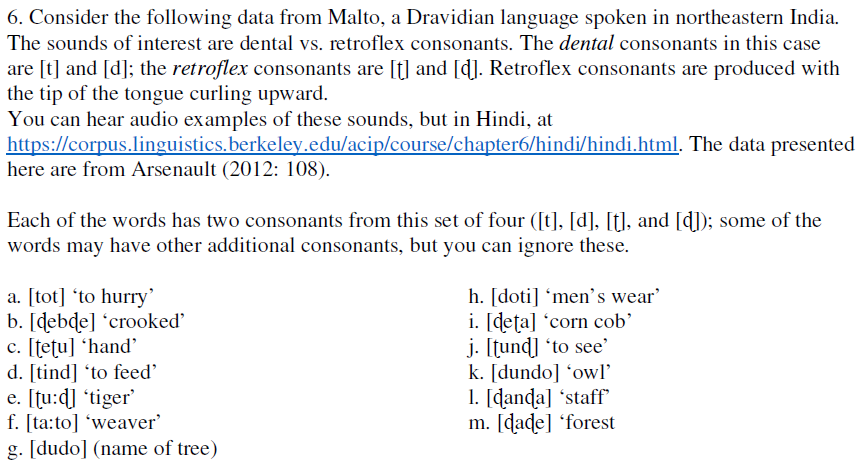
\includegraphics{../images/malto.png}
\end{figure}

\newpage

{\large Question 5}\\

Topic: Phonological Relationships and Analysis\\
Source: Week 6 Handout, Question 11\\

What do the two signs below tell you about the phonological status of \underline{handshape} in ASL, and why?\\

\begin{figure}[H]
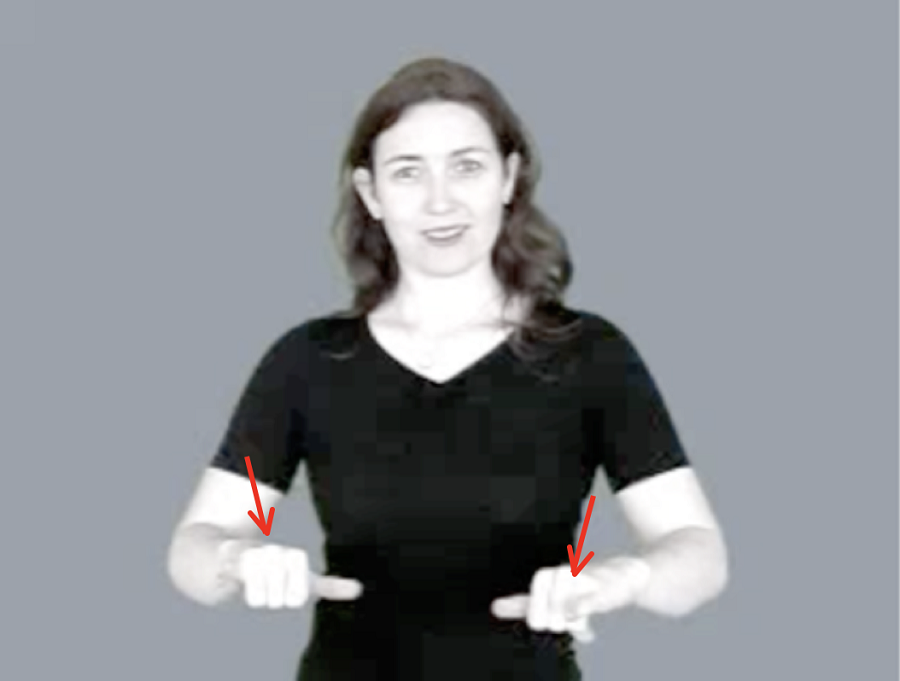
\includegraphics{../images/asl_stay.png}
\caption{STAY}
\end{figure}
\begin{figure}[H]
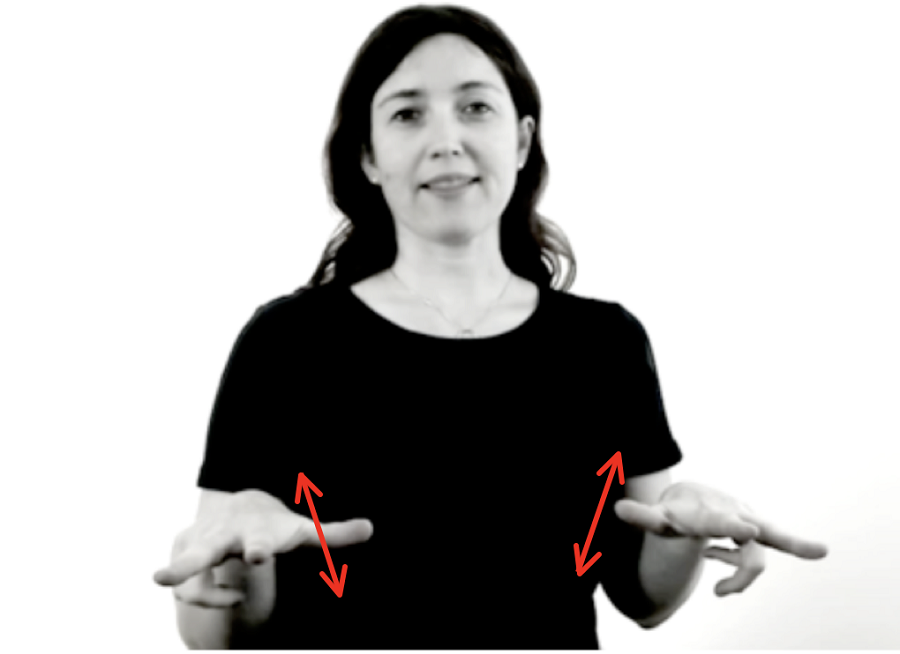
\includegraphics{../images/asl_awkward.png}
\caption{AWKWARD}
\end{figure}

\newpage

\begin{center}
\textbf{{\color{red}{\HUGE END OF EXAM}}}\\

\end{center}
\newpage

\begin{center}
\textbf{{\color{blue}{\HUGE START OF EXAM\\}}}

\textbf{{\color{blue}{\HUGE Student ID: 11061\\}}}

\textbf{{\color{blue}{\HUGE \\}}}

\end{center}
\newpage

{\large Question 1}\\

Topic: Transcription\\
Source: Quiz 1, Question 10\\

Explain whether this word either does or does not have an [ʃ] sound in it, and why the spelling and pronunciation either do or do not align.\\

<facial>


\newpage

{\large Question 2}\\

Topic: Articulatory Phonetics\\
Source: Week 3 Discussion\\

Assuming a Standard North American English inventory, does this vowel need to have tenseness specified if you're giving a prose description? Why or why not?\\

{[ɑ]}


\newpage

{\large Question 3}\\

Topic: Phonological Features\\
Source: Homework 2, Question 1\\

Explain which sound should be removed to make this a natural class (assuming SNAE, except that there are no diphthongs, no [ə] or [ʌ], no syllabic consonants, and no [w̥]), and what the minimum set of features would be to describe the resulting natural class.\\

{[i]}, {[ɪ]}, {[ɛ]}, {[u]}, {[ʊ]}


\newpage

{\large Question 4}\\

Topic: Skewed Distributions\\
Source: Week 5 Handout, Question 7\\

Explain how you would go about looking for co-occurrence restrictions in bi-syllabic signs in ASL. (Refer to the data that follows.)\\

\begin{figure}[H]
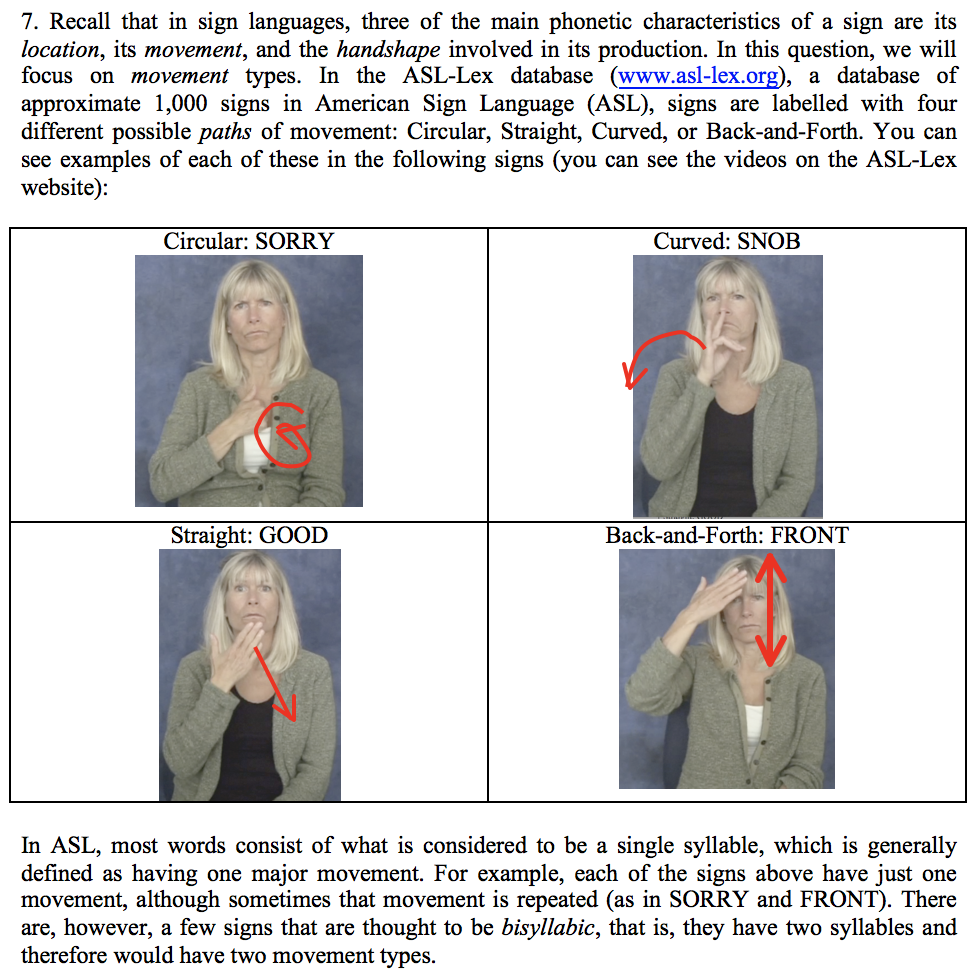
\includegraphics{../images/ASL_movement.png}
\end{figure}

\newpage

{\large Question 5}\\

Topic: Phonological Relationships and Analysis\\
Source: Week 7 Handout, Question 12\\

What is the basic analysis of oral and nasal vowels in this dataset, and what are the key pieces of evidence?\\

\begin{figure}[H]
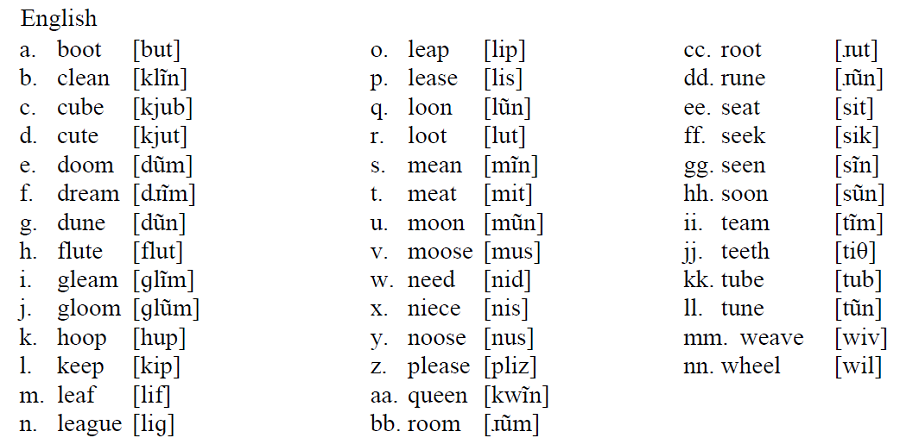
\includegraphics{../images/english12.png}
\end{figure}

\newpage

\begin{center}
\textbf{{\color{red}{\HUGE END OF EXAM}}}\\

\end{center}
\newpage

\begin{center}
\textbf{{\color{blue}{\HUGE START OF EXAM\\}}}

\textbf{{\color{blue}{\HUGE Student ID: 11196\\}}}

\textbf{{\color{blue}{\HUGE \\}}}

\end{center}
\newpage

{\large Question 1}\\

Topic: Transcription\\
Source: Quiz 1, Question 10\\

Explain whether this word either does or does not have an [ʃ] sound in it, and why the spelling and pronunciation either do or do not align.\\

<bassoon>


\newpage

{\large Question 2}\\

Topic: Articulatory Phonetics\\
Source: Quiz 2, Question 6\\

In the pronunciation of this word, which sounds are obstruents and which are sonorants? Explain your answer.\\

<language>


\newpage

{\large Question 3}\\

Topic: Phonological Features\\
Source: Week 4 Discussion\\

Explain why the given feature's value varies across this set of sounds.\\

{[anterior]}

fricatives


\newpage

{\large Question 4}\\

Topic: Skewed Distributions\\
Source: Week 5 Handout, Question 7\\

Explain how you would go about looking for co-occurrence restrictions in bi-syllabic signs in ASL. (Refer to the data that follows.)\\

\begin{figure}[H]
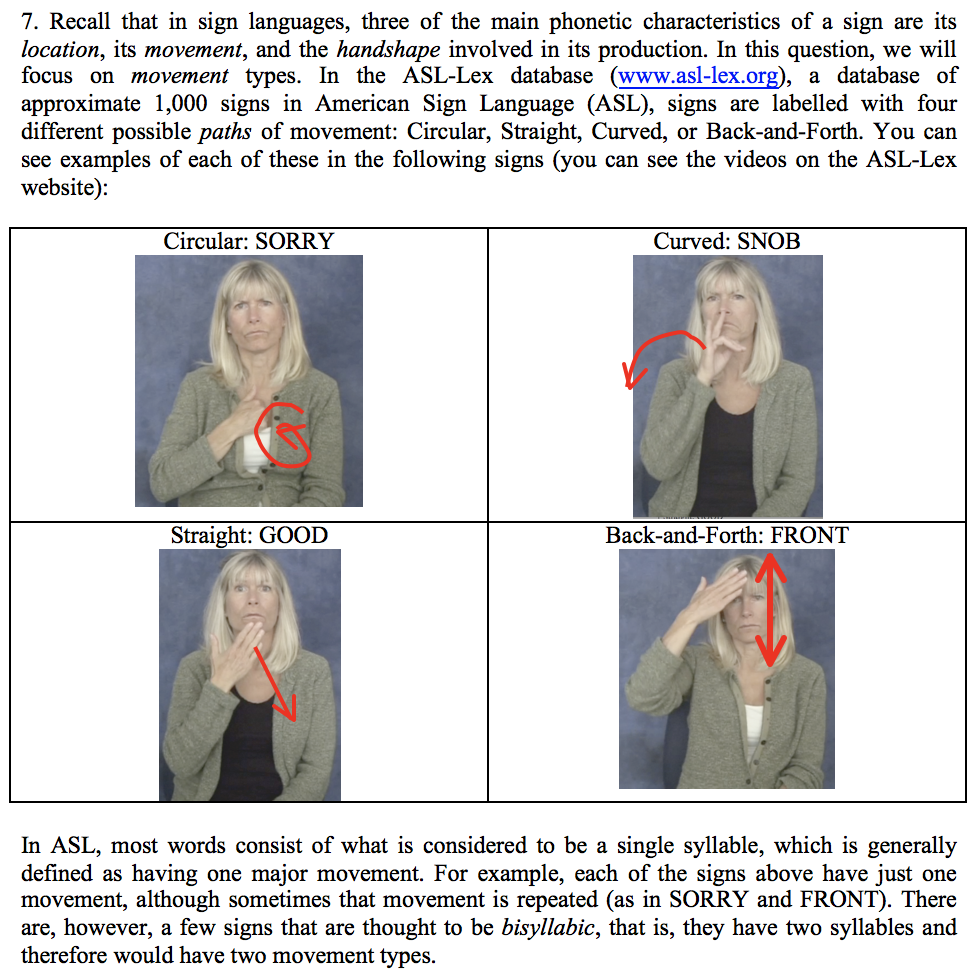
\includegraphics{../images/ASL_movement.png}
\end{figure}

\newpage

{\large Question 5}\\

Topic: Phonological Relationships and Analysis\\
Source: Week 7 Handout, Question 9\\

What is the basic analysis of vowel length in this dataset, and what are the key pieces of evidence?\\

\begin{figure}[H]
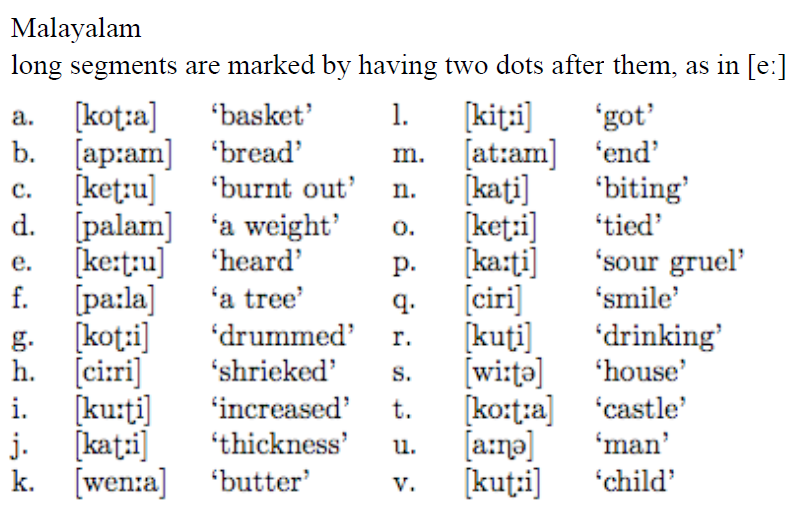
\includegraphics{../images/malayalam.png}
\end{figure}

\newpage

\begin{center}
\textbf{{\color{red}{\HUGE END OF EXAM}}}\\

\end{center}
\newpage

\begin{center}
\textbf{{\color{blue}{\HUGE START OF EXAM\\}}}

\textbf{{\color{blue}{\HUGE Student ID: 11661\\}}}

\textbf{{\color{blue}{\HUGE \\}}}

\end{center}
\newpage

{\large Question 1}\\

Topic: Transcription\\
Source: Week 2 Handout, Part II, Question 3\\

Explain why people might legitimately disagree about how many sounds this particular word contains.\\

<worse>


\newpage

{\large Question 2}\\

Topic: Articulatory Phonetics\\
Source: Week 3 Handout, Question 3\\

Explain why the additional vowel below either does or does not belong in the phonetic natural class defined by the original set of SNAE vowels.\\

Original set: {[ɛ]}, {[ɪ]}, {[ʊ]}, {[ɔ]}

Addition: {[ɑ]}


\newpage

{\large Question 3}\\

Topic: Phonological Features\\
Source: Week 4 Discussion\\

Explain why the given feature's value varies across this set of sounds.\\

{[anterior]}

fricatives


\newpage

{\large Question 4}\\

Topic: Skewed Distributions\\
Source: Quiz 4, Question 3\\

L$_X$ (Language X) has three vowels, [i], [a], and [u]. L$_X$ has tetra-syllabic roots. If L$_X$ does not allow non-identical high vowels to co-occur, which one of the following tetra-syllabic vocalic sequences do you predict to be unattested in L$_X$? Explain why.\\

\begin{itemize} \item {[i...i...u...u]} \item {[a...a...i...i]} \item {[u...u...u...u]} \item {[i...i...i...a]} \end{itemize}


\newpage

{\large Question 5}\\

Topic: Phonological Relationships and Analysis\\
Source: Week 6 Handout, Question 11\\

What do the two signs below tell you about the phonological status of \underline{handshape} in ASL, and why?\\

\begin{figure}[H]
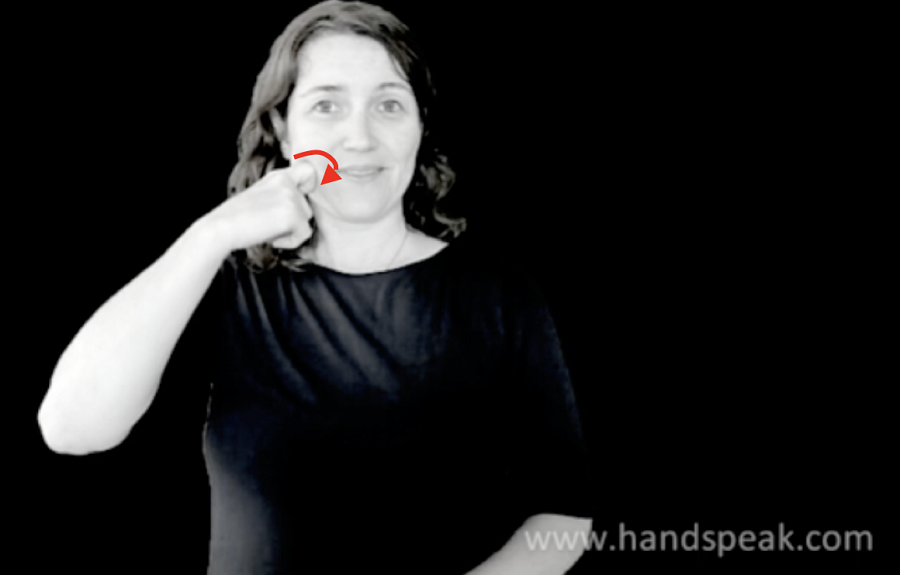
\includegraphics{../images/asl_apple.png}
\caption{APPLE}
\end{figure}
\begin{figure}[H]
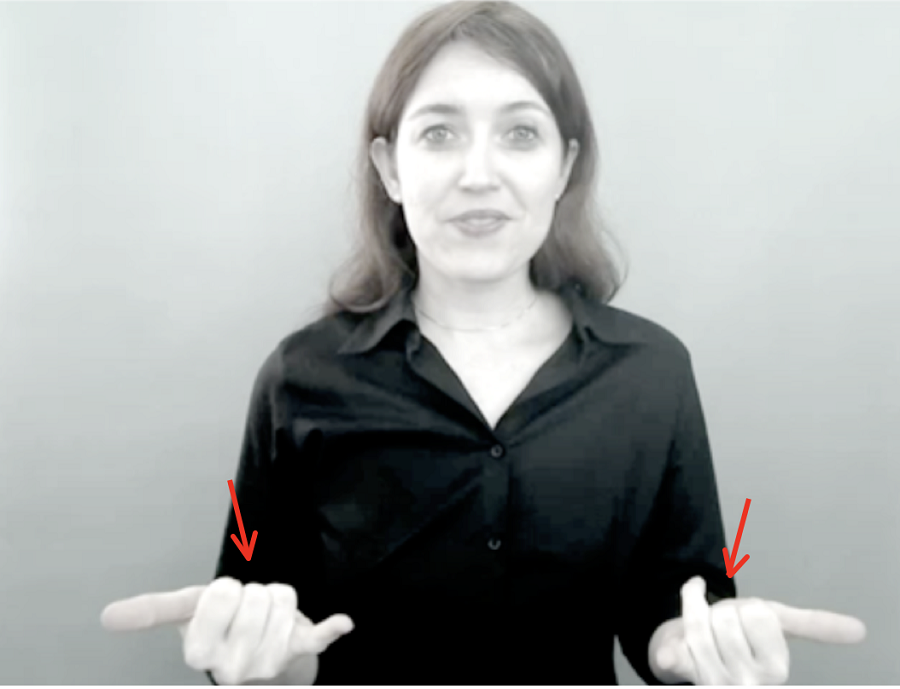
\includegraphics{../images/asl_now.png}
\caption{NOW}
\end{figure}

\newpage

\begin{center}
\textbf{{\color{red}{\HUGE END OF EXAM}}}\\

\end{center}
\newpage

\begin{center}
\textbf{{\color{blue}{\HUGE START OF EXAM\\}}}

\textbf{{\color{blue}{\HUGE Student ID: 11925\\}}}

\textbf{{\color{blue}{\HUGE \\}}}

\end{center}
\newpage

{\large Question 1}\\

Topic: Transcription\\
Source: Week 2 Handout, Part II\\

Is this a reasonable transcription of this word? Explain why.\\

<mouse>: {[mɔɪs]}


\newpage

{\large Question 2}\\

Topic: Articulatory Phonetics\\
Source: Week 3 Handout, Question 13\\

Explain why this image does or does not match the description.\\

\begin{itemize} \item A two-handed sign. \item Location: In front of signer’s chin. \item Handshape: Starts with an “L” shape; index finger and thumb come together during the sign. \item Movement: Hands start crossed and then move away from each other horizontally. \end{itemize}

\begin{figure}[H]
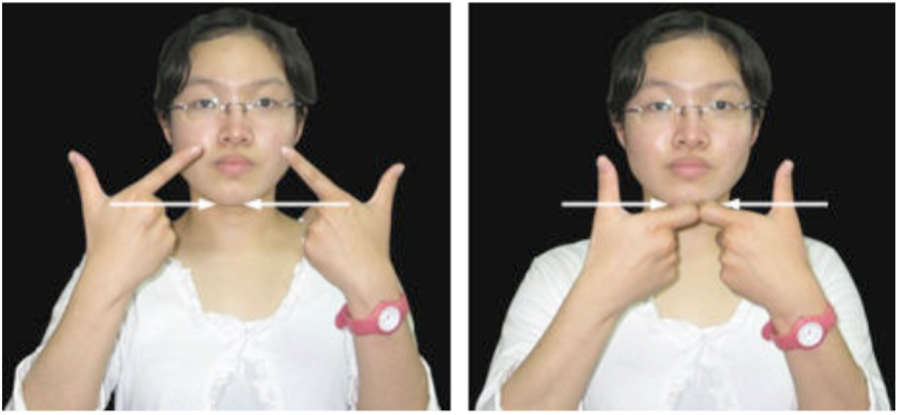
\includegraphics{../images/taiwansign_fit.png}
\caption{FIT}
\end{figure}

\newpage

{\large Question 3}\\

Topic: Phonological Features\\
Source: Homework 2, Question 1\\

Explain which sound should be removed to make this a natural class (assuming SNAE, except that there are no diphthongs, no [ə] or [ʌ], no syllabic consonants, and no [w̥]), and what the minimum set of features would be to describe the resulting natural class.\\

{[i]}, {[ɪ]}, {[ɛ]}, {[u]}, {[ʊ]}


\newpage

{\large Question 4}\\

Topic: Skewed Distributions\\
Source: Week 5 Handout, Question 6\\

Explain why the following table would not be a good way of organizing the data for Malto.\\

\begin{figure}[H]
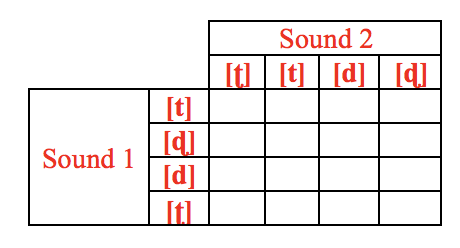
\includegraphics{../images/Malto_table_bad.png}
\end{figure}

\newpage

{\large Question 5}\\

Topic: Phonological Relationships and Analysis\\
Source: Week 7 Handout, Question 9\\

What is the basic analysis of vowel length in this dataset, and what are the key pieces of evidence?\\

\begin{figure}[H]
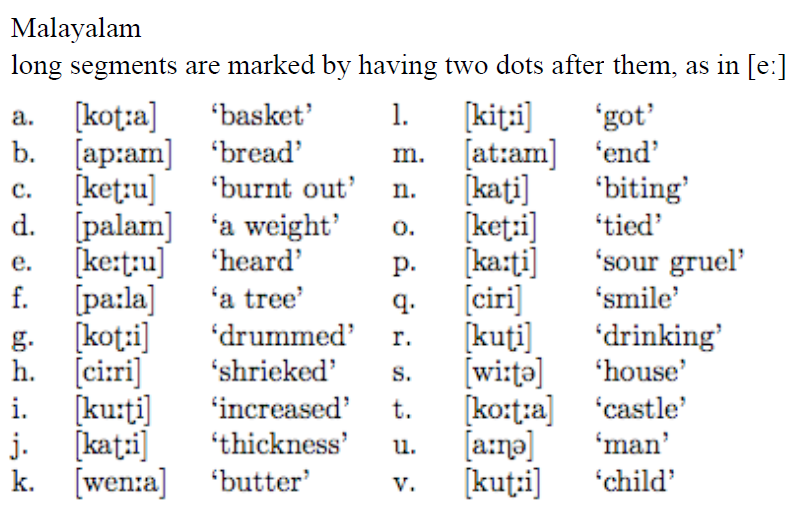
\includegraphics{../images/malayalam.png}
\end{figure}

\newpage

\begin{center}
\textbf{{\color{red}{\HUGE END OF EXAM}}}\\

\end{center}
\newpage

\begin{center}
\textbf{{\color{blue}{\HUGE START OF EXAM\\}}}

\textbf{{\color{blue}{\HUGE Student ID: 12377\\}}}

\textbf{{\color{blue}{\HUGE \\}}}

\end{center}
\newpage

{\large Question 1}\\

Topic: Transcription\\
Source: Week 2 Handout, Part II, Question 11\\

How would this word be transcribed?\\ (Kathleen will then ask a follow-up question about your transcription.)\\

<cough>


\newpage

{\large Question 2}\\

Topic: Articulatory Phonetics\\
Source: Week 3 Handout, Question 7\\

Is the symbol given a reasonable way to transcribe any of the sounds described below? If so, which one? If not, why not? Explain your answer.\\

{[n]}

\begin{itemize} \item voiceless palatal affricate \item voiced velar nasal \item voiceless glottal fricative \item voiced labiodental fricative \item voiced interdental fricative \item voiced palatal fricative \end{itemize}


\newpage

{\large Question 3}\\

Topic: Phonological Features\\
Source: Quiz 3, Question 12\\

Explain how you figure out which feature is involved in the process of umlaut shown below.\\

\begin{figure}[H]
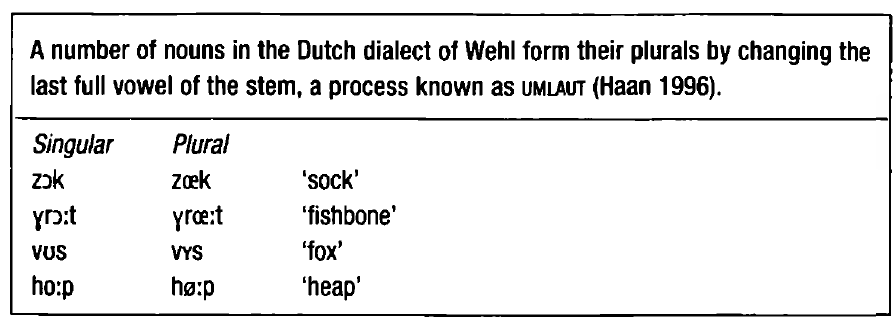
\includegraphics{../images/dutch.png}
\end{figure}

\newpage

{\large Question 4}\\

Topic: Skewed Distributions\\
Source: Week 5 Handout, Question 1\\

Explain why we think that languages are not random in terms of their phonology.\\


\newpage

{\large Question 5}\\

Topic: Phonological Relationships and Analysis\\
Source: Week 6 Handout, Question 11\\

What do the two signs below tell you about the phonological status of \underline{handshape} in ASL, and why?\\

\begin{figure}[H]
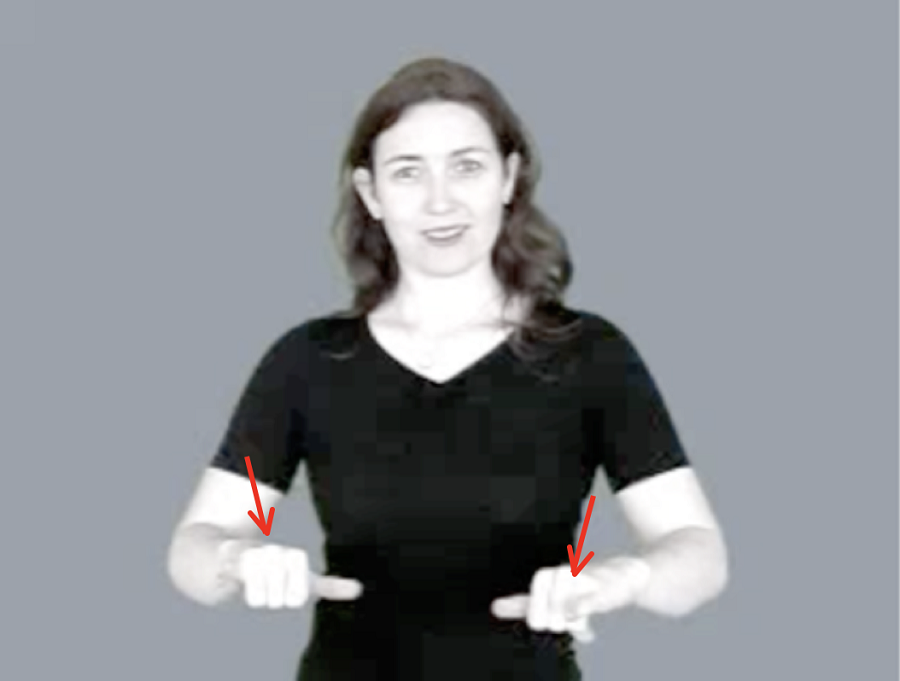
\includegraphics{../images/asl_stay.png}
\caption{STAY}
\end{figure}
\begin{figure}[H]
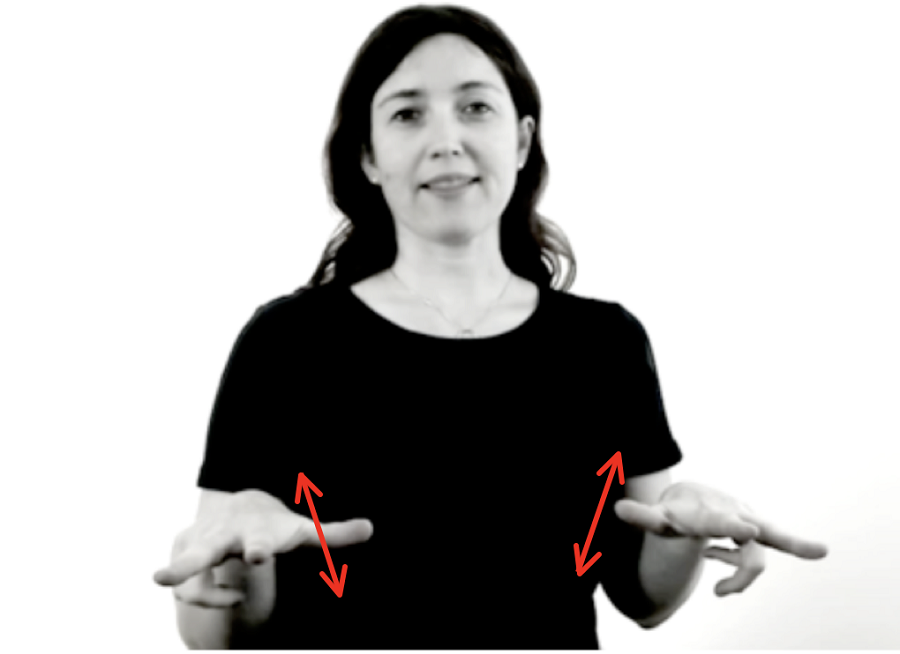
\includegraphics{../images/asl_awkward.png}
\caption{AWKWARD}
\end{figure}

\newpage

\begin{center}
\textbf{{\color{red}{\HUGE END OF EXAM}}}\\

\end{center}
\newpage

\begin{center}
\textbf{{\color{blue}{\HUGE START OF EXAM\\}}}

\textbf{{\color{blue}{\HUGE Student ID: 12991\\}}}

\textbf{{\color{blue}{\HUGE \\}}}

\end{center}
\newpage

{\large Question 1}\\

Topic: Transcription\\
Source: Week 2 Handout, Part II, Question 11\\

How would this word be transcribed?\\ (Kathleen will then ask a follow-up question about your transcription.)\\

<goat>


\newpage

{\large Question 2}\\

Topic: Articulatory Phonetics\\
Source: Homework 1, Question 3(b)\\

Explain why this is or is not a complete phonetic natural class in standard North American English.\\

{[ɔ]}, {[ʊ]}, {[u]}, {[oʊ]}


\newpage

{\large Question 3}\\

Topic: Phonological Features\\
Source: Quiz 3, Question 6\\

Explain why this is an incorrect statement.\\

Nasal consonants are {[-continuant]}, because they cannot be produced for an extended period of time.


\newpage

{\large Question 4}\\

Topic: Skewed Distributions\\
Source: Week 5 Handout, Question 6\\

If I gave you a new word in Malto, [di\_\_u], would it be possible to predict whether it's [d] or [t] that goes in the blank? Explain why or why not.\\

\begin{figure}[H]
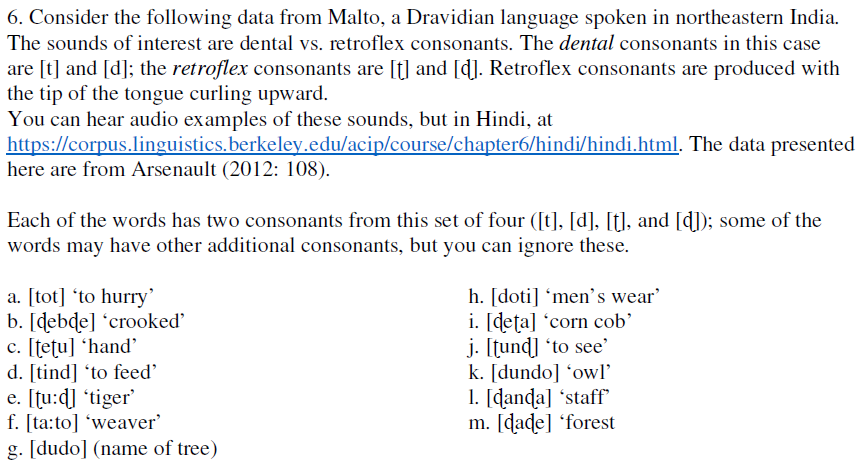
\includegraphics{../images/malto.png}
\end{figure}

\newpage

{\large Question 5}\\

Topic: Phonological Relationships and Analysis\\
Source: Week 7 Handout, Question 12\\

What is the basic analysis of oral and nasal vowels in this dataset, and what are the key pieces of evidence?\\

\begin{figure}[H]
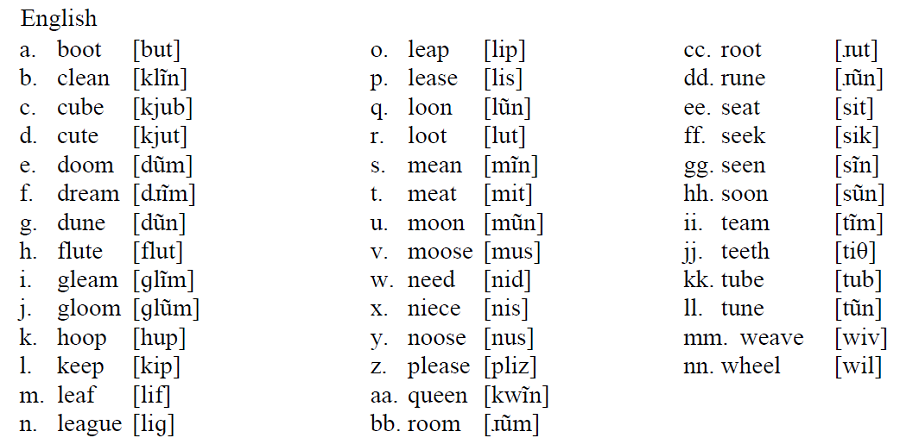
\includegraphics{../images/english12.png}
\end{figure}

\newpage

\begin{center}
\textbf{{\color{red}{\HUGE END OF EXAM}}}\\

\end{center}
\newpage

\begin{center}
\textbf{{\color{blue}{\HUGE START OF EXAM\\}}}

\textbf{{\color{blue}{\HUGE Student ID: 13570\\}}}

\textbf{{\color{blue}{\HUGE \\}}}

\end{center}
\newpage

{\large Question 1}\\

Topic: Transcription\\
Source: Quiz 1, Question 10\\

Explain whether this word either does or does not have an [ʃ] sound in it, and why the spelling and pronunciation either do or do not align.\\

<meticulous>


\newpage

{\large Question 2}\\

Topic: Articulatory Phonetics\\
Source: Homework 1, Question 3(b)\\

Explain why this is or is not a complete phonetic natural class in standard North American English.\\

{[ɔ]}, {[ʊ]}, {[u]}, {[oʊ]}


\newpage

{\large Question 3}\\

Topic: Phonological Features\\
Source: Week 4 Discussion\\

Explain what the given feature’s value is for this class of sounds, and why.\\

{[approximant]}

nasals


\newpage

{\large Question 4}\\

Topic: Skewed Distributions\\
Source: Week 5 Handout, Question 7\\

Explain how you would go about looking for co-occurrence restrictions in bi-syllabic signs in ASL. (Refer to the data that follows.)\\

\begin{figure}[H]
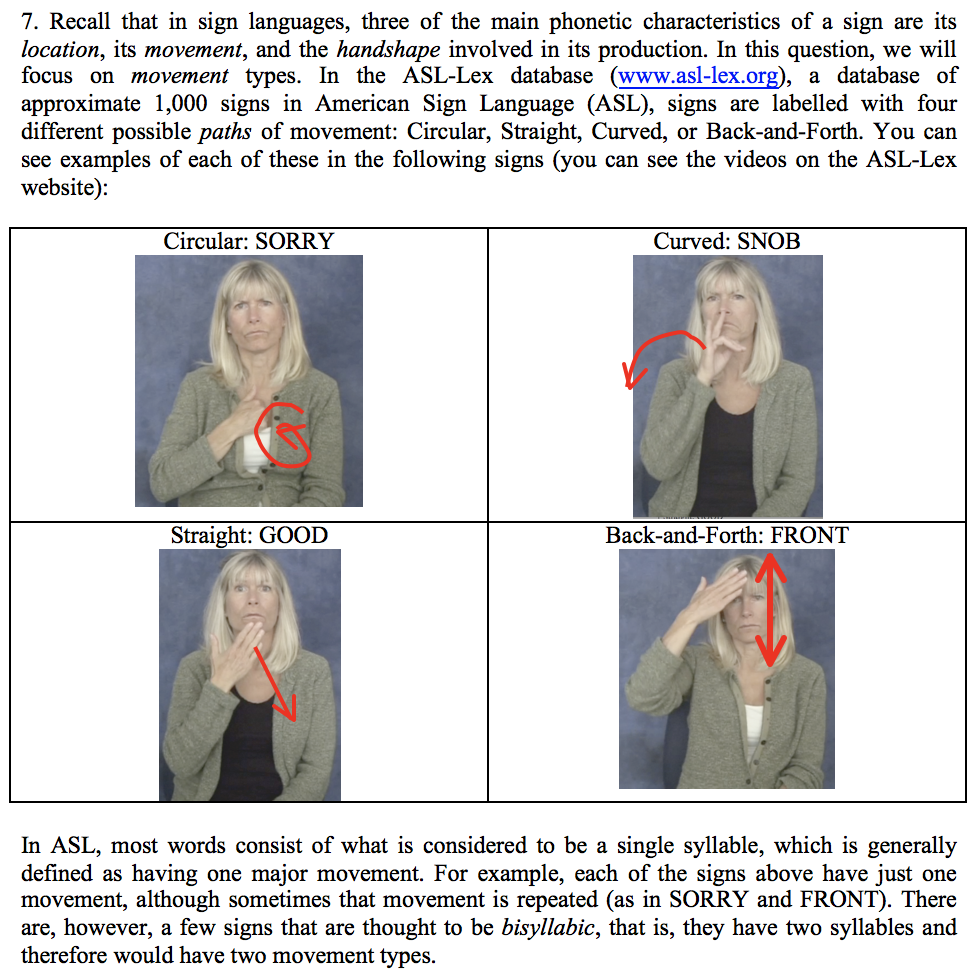
\includegraphics{../images/ASL_movement.png}
\end{figure}

\newpage

{\large Question 5}\\

Topic: Phonological Relationships and Analysis\\
Source: Week 7 Handout, Question 12\\

What is the basic analysis of oral and nasal vowels in this dataset, and what are the key pieces of evidence?\\

\begin{figure}[H]
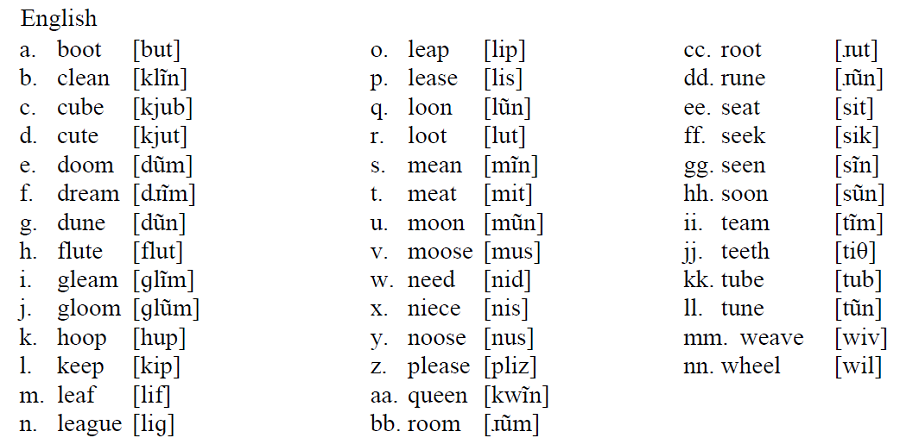
\includegraphics{../images/english12.png}
\end{figure}

\newpage

\begin{center}
\textbf{{\color{red}{\HUGE END OF EXAM}}}\\

\end{center}
\newpage

\begin{center}
\textbf{{\color{blue}{\HUGE START OF EXAM\\}}}

\textbf{{\color{blue}{\HUGE Student ID: 15082\\}}}

\textbf{{\color{blue}{\HUGE \\}}}

\end{center}
\newpage

{\large Question 1}\\

Topic: Transcription\\
Source: Week 2 Handout, Part II, Question 2\\

Explain why people might legitimately disagree about how many sounds this particular word contains.\\

<goat>


\newpage

{\large Question 2}\\

Topic: Articulatory Phonetics\\
Source: Week 3 Handout, Question 9\\

Explain how to figure out what the sound being produced is in this diagram.\\

\begin{figure}[H]
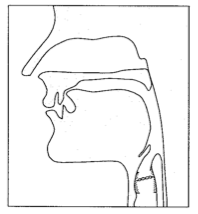
\includegraphics{../images/sagittal_z.png}
\end{figure}

\newpage

{\large Question 3}\\

Topic: Phonological Features\\
Source: Quiz 3, Question 12\\

Explain how you figure out which feature is involved in the process of umlaut shown below.\\

\begin{figure}[H]
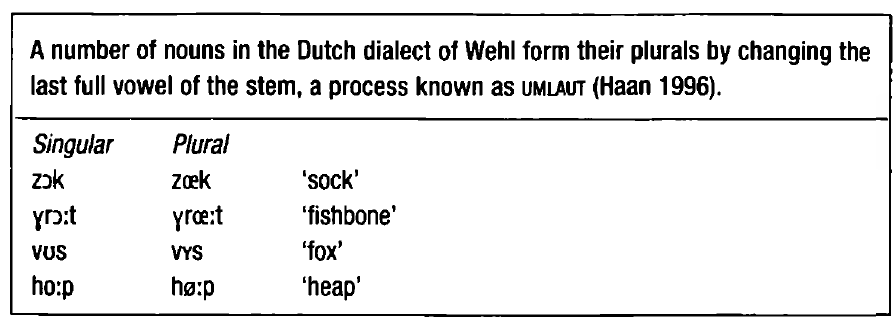
\includegraphics{../images/dutch.png}
\end{figure}

\newpage

{\large Question 4}\\

Topic: Skewed Distributions\\
Source: Quiz 4, Question 1\\

L$_X$ (Language X) has three vowels, [i], [a], and [u]. It has bi-syllabic roots like Kikuyu. It does not allow non-identical high vowels to co-occur. Of the following nine logically possible vocalic sequences, which ones should be unattested in L$_X$? Explain why.\\

\begin{itemize} \item {[i...i]} \item {[i...a]} \item {[i...u]} \item {[a...i]} \item {[a...a]} \item {[a...u]} \item {[u...i]} \item {[u...a]} \item {[u...u]} \end{itemize}


\newpage

{\large Question 5}\\

Topic: Phonological Relationships and Analysis\\
Source: Week 7 Handout, Question 12\\

What is the basic analysis of oral and nasal vowels in this dataset, and what are the key pieces of evidence?\\

\begin{figure}[H]
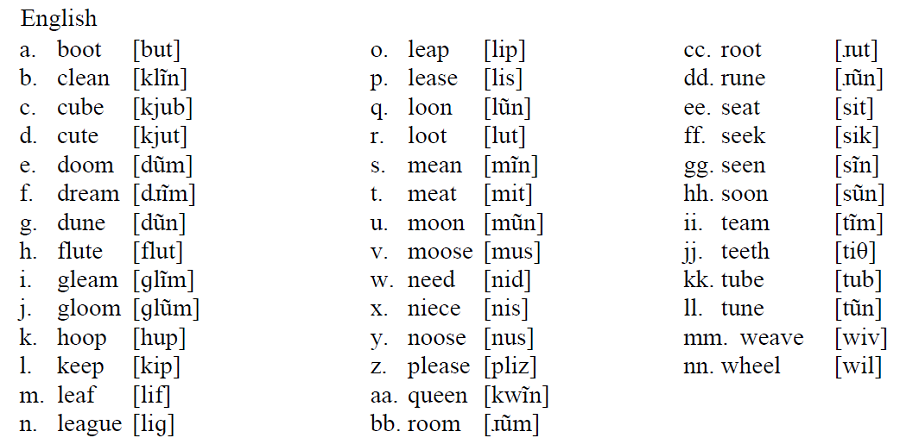
\includegraphics{../images/english12.png}
\end{figure}

\newpage

\begin{center}
\textbf{{\color{red}{\HUGE END OF EXAM}}}\\

\end{center}
\newpage

\begin{center}
\textbf{{\color{blue}{\HUGE START OF EXAM\\}}}

\textbf{{\color{blue}{\HUGE Student ID: 16464\\}}}

\textbf{{\color{blue}{\HUGE \\}}}

\end{center}
\newpage

{\large Question 1}\\

Topic: Transcription\\
Source: Week 2 Handout, Part II, Question 11\\

How would this word be transcribed?\\ (Kathleen will then ask a follow-up question about your transcription.)\\

<goat>


\newpage

{\large Question 2}\\

Topic: Articulatory Phonetics\\
Source: Week 3 Handout, Question 7\\

Is the symbol given a reasonable way to transcribe any of the sounds described below? If so, which one? If not, why not? Explain your answer.\\

{[v]}

\begin{itemize} \item voiceless palatal affricate \item voiced velar nasal \item voiceless glottal fricative \item voiced labiodental fricative \item voiced interdental fricative \item voiced palatal fricative \end{itemize}


\newpage

{\large Question 3}\\

Topic: Phonological Features\\
Source: Week 4 Discussion\\

Explain what the given feature’s value is for this class of sounds, and why.\\

{[approximant]}

nasals


\newpage

{\large Question 4}\\

Topic: Skewed Distributions\\
Source: Week 5 Handout, Question 7\\

Explain how you would go about looking for co-occurrence restrictions in bi-syllabic signs in ASL. (Refer to the data that follows.)\\

\begin{figure}[H]
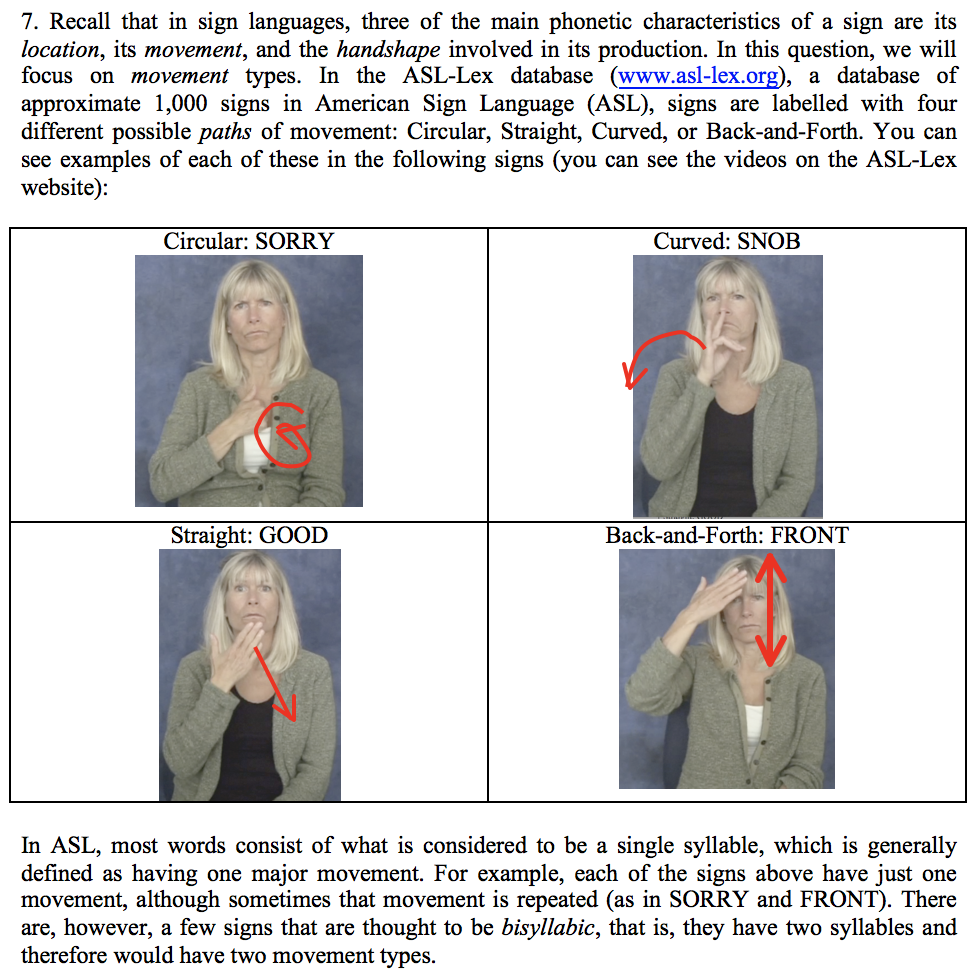
\includegraphics{../images/ASL_movement.png}
\end{figure}

\newpage

{\large Question 5}\\

Topic: Phonological Relationships and Analysis\\
Source: Week 7 Handout, Question 9\\

What is the basic analysis of vowel length in this dataset, and what are the key pieces of evidence?\\

\begin{figure}[H]
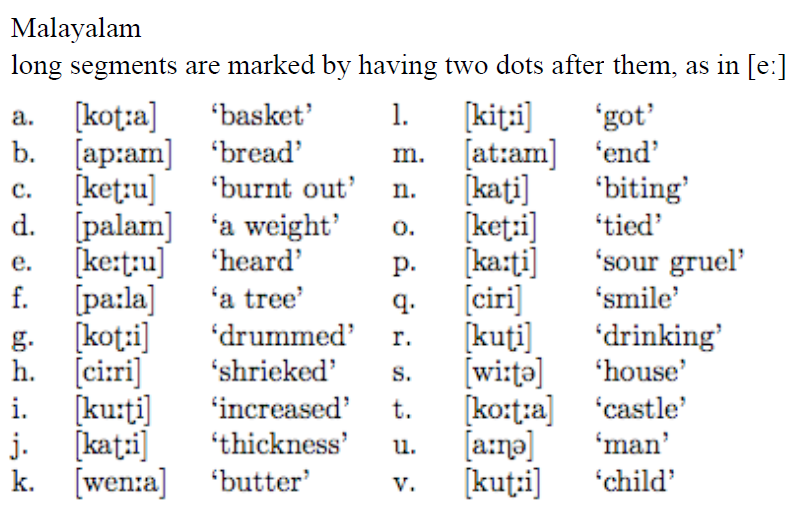
\includegraphics{../images/malayalam.png}
\end{figure}

\newpage

\begin{center}
\textbf{{\color{red}{\HUGE END OF EXAM}}}\\

\end{center}
\newpage

\begin{center}
\textbf{{\color{blue}{\HUGE START OF EXAM\\}}}

\textbf{{\color{blue}{\HUGE Student ID: 16758\\}}}

\textbf{{\color{blue}{\HUGE \\}}}

\end{center}
\newpage

{\large Question 1}\\

Topic: Transcription\\
Source: Week 2 Handout, Part II, Question 3\\

Explain why people might legitimately disagree about how many sounds this particular word contains.\\

<better>


\newpage

{\large Question 2}\\

Topic: Articulatory Phonetics\\
Source: Week 3 Handout, Question 13\\

Explain why this image does or does not match the description.\\

\begin{itemize} \item A one-handed sign. \item Location: At the signer’s nose. \item Handshape: Starts with index finger extended; finger folds down into a “hook” shape during the sign; then straightens and repeats the folding. \item Movement: No movement other than the change in handshape. \end{itemize}

\begin{figure}[H]
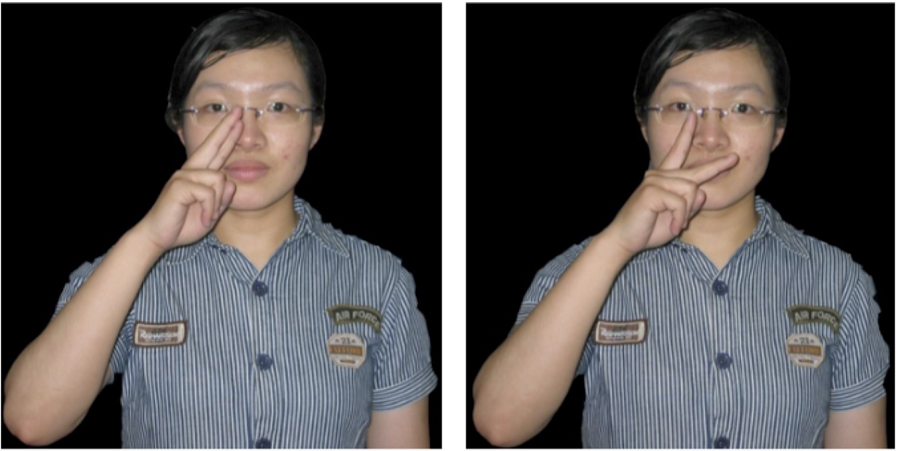
\includegraphics{../images/taiwansign_wrong.png}
\caption{WRONG}
\end{figure}

\newpage

{\large Question 3}\\

Topic: Phonological Features\\
Source: Week 4 Discussion\\

Explain why phonological features are used instead of phonetic characteristics in analyzing datasets.\\


\newpage

{\large Question 4}\\

Topic: Skewed Distributions\\
Source: Week 5 Handout, Question 3\\

What evidence is there that there is a pattern in these data, assuming that these are the only CV and VC sequences that occur in some language?\\

{[sa]}, {[ʃi]}, {[za]}, {[ʒi]}, {[as]}, {[iʃ]}, {[az]}, {[iʒ]}


\newpage

{\large Question 5}\\

Topic: Phonological Relationships and Analysis\\
Source: Week 7 Handout, Question 9\\

What is the basic analysis of vowel length in this dataset, and what are the key pieces of evidence?\\

\begin{figure}[H]
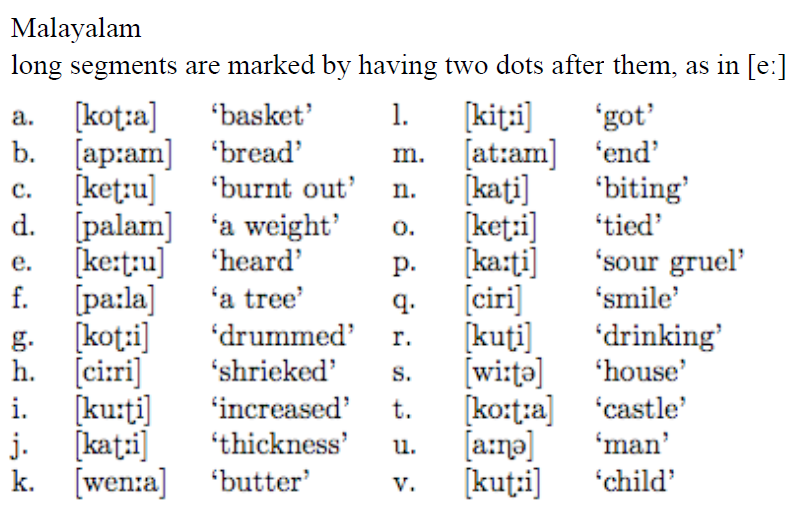
\includegraphics{../images/malayalam.png}
\end{figure}

\newpage

\begin{center}
\textbf{{\color{red}{\HUGE END OF EXAM}}}\\

\end{center}
\newpage

\begin{center}
\textbf{{\color{blue}{\HUGE START OF EXAM\\}}}

\textbf{{\color{blue}{\HUGE Student ID: 16922\\}}}

\textbf{{\color{blue}{\HUGE \\}}}

\end{center}
\newpage

{\large Question 1}\\

Topic: Transcription\\
Source: Week 2 Handout, Part II, Question 11\\

How would this word be transcribed?\\ (Kathleen will then ask a follow-up question about your transcription.)\\

<bird>


\newpage

{\large Question 2}\\

Topic: Articulatory Phonetics\\
Source: Week 3 Discussion\\

Describe what the tongue would do / where it would move during each of the vowels in this word.\\

<vacuum>


\newpage

{\large Question 3}\\

Topic: Phonological Features\\
Source: Quiz 3, Question 12\\

Explain how you figure out which feature is involved in the process of umlaut shown below.\\

\begin{figure}[H]
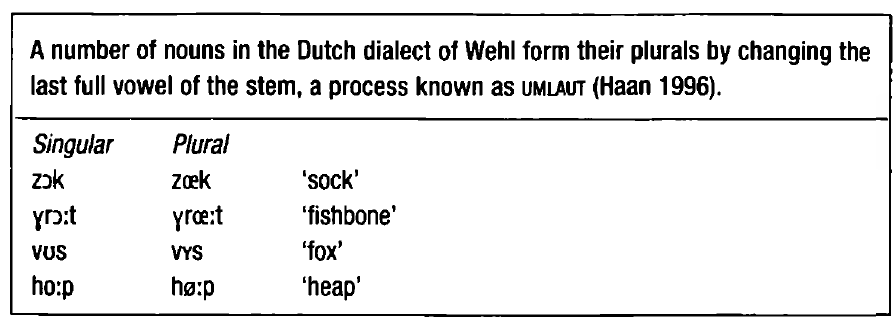
\includegraphics{../images/dutch.png}
\end{figure}

\newpage

{\large Question 4}\\

Topic: Skewed Distributions\\
Source: Quiz 4, Question 1\\

L$_X$ (Language X) has three vowels, [i], [a], and [u]. It has bi-syllabic roots like Kikuyu. It does not allow non-identical high vowels to co-occur. Of the following nine logically possible vocalic sequences, which ones should be unattested in L$_X$? Explain why.\\

\begin{itemize} \item {[i...i]} \item {[i...a]} \item {[i...u]} \item {[a...i]} \item {[a...a]} \item {[a...u]} \item {[u...i]} \item {[u...a]} \item {[u...u]} \end{itemize}


\newpage

{\large Question 5}\\

Topic: Phonological Relationships and Analysis\\
Source: Week 6 Handout, Question 11\\

What do the two signs below tell you about the phonological status of \underline{handshape} in ASL, and why?\\

\begin{figure}[H]
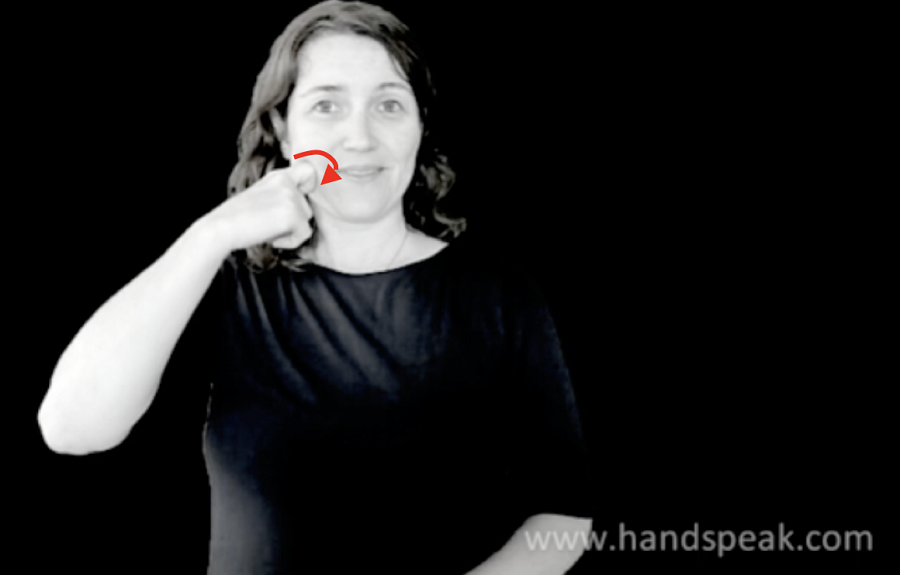
\includegraphics{../images/asl_apple.png}
\caption{APPLE}
\end{figure}
\begin{figure}[H]
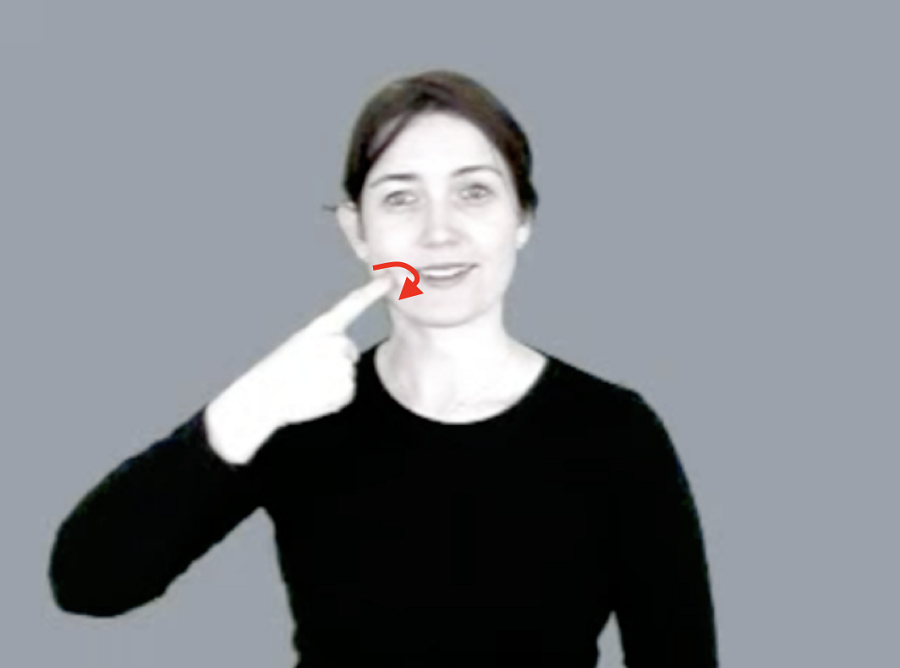
\includegraphics{../images/asl_candy.png}
\caption{CANDY}
\end{figure}

\newpage

\begin{center}
\textbf{{\color{red}{\HUGE END OF EXAM}}}\\

\end{center}
\newpage

\begin{center}
\textbf{{\color{blue}{\HUGE START OF EXAM\\}}}

\textbf{{\color{blue}{\HUGE Student ID: 17335\\}}}

\textbf{{\color{blue}{\HUGE \\}}}

\end{center}
\newpage

{\large Question 1}\\

Topic: Transcription\\
Source: Week 2 Handout, Part II, Question 11\\

How would this word be transcribed?\\ (Kathleen will then ask a follow-up question about your transcription.)\\

<wealth>


\newpage

{\large Question 2}\\

Topic: Articulatory Phonetics\\
Source: Week 3 Discussion\\

Describe what the tongue would do / where it would move during each of the vowels in this word.\\

<follow>


\newpage

{\large Question 3}\\

Topic: Phonological Features\\
Source: Quiz 3, Question 12\\

Explain how you figure out which feature is involved in the process of umlaut shown below.\\

\begin{figure}[H]
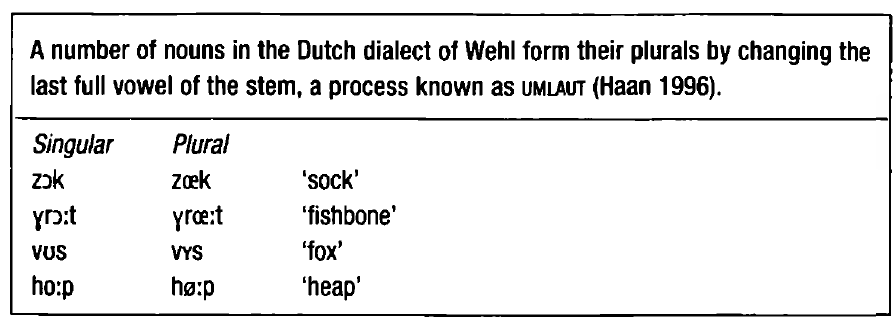
\includegraphics{../images/dutch.png}
\end{figure}

\newpage

{\large Question 4}\\

Topic: Skewed Distributions\\
Source: Quiz 4, Question 2\\

L$_X$ (Language X) has three vowels, [i], [a], and [u]. L$_X$ has tri-syllabic roots. If L$_X$ does not allow non-identical high vowels to co-occur, which one of the following tri-syllabic vocalic sequences do you predict to be unattested in L$_X$? Explain why.\\

\begin{itemize} \item {[u...i...a]} \item {[a...i...a]} \item {[u...u...a]} \item {[a...i...i]} \end{itemize}


\newpage

{\large Question 5}\\

Topic: Phonological Relationships and Analysis\\
Source: Week 7 Handout, Question 12\\

What is the basic analysis of oral and nasal vowels in this dataset, and what are the key pieces of evidence?\\

\begin{figure}[H]
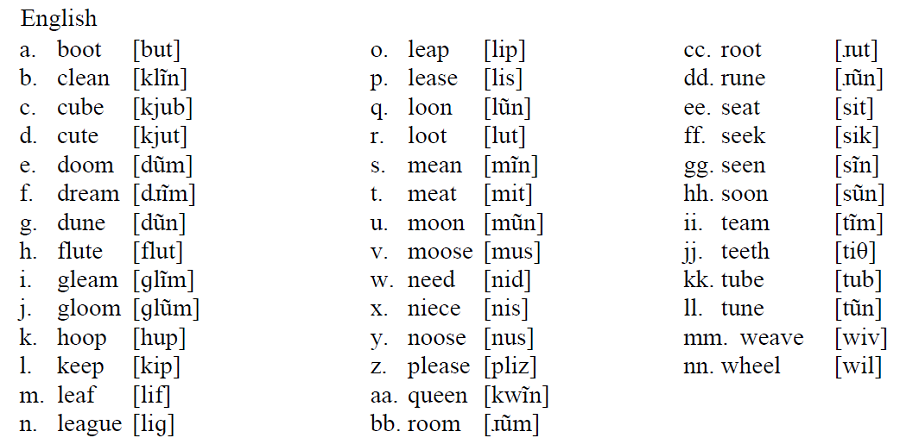
\includegraphics{../images/english12.png}
\end{figure}

\newpage

\begin{center}
\textbf{{\color{red}{\HUGE END OF EXAM}}}\\

\end{center}
\newpage

\begin{center}
\textbf{{\color{blue}{\HUGE START OF EXAM\\}}}

\textbf{{\color{blue}{\HUGE Student ID: 17357\\}}}

\textbf{{\color{blue}{\HUGE \\}}}

\end{center}
\newpage

{\large Question 1}\\

Topic: Transcription\\
Source: Week 2 Handout, Part II, Question 11\\

How would this word be transcribed?\\ (Kathleen will then ask a follow-up question about your transcription.)\\

<segment>


\newpage

{\large Question 2}\\

Topic: Articulatory Phonetics\\
Source: Week 3 Handout, Question 7\\

Is the symbol given a reasonable way to transcribe any of the sounds described below? If so, which one? If not, why not? Explain your answer.\\

{[ʒ]}

\begin{itemize} \item voiceless palatal affricate \item voiced velar nasal \item voiceless glottal fricative \item voiced labiodental fricative \item voiced interdental fricative \item voiced palatal fricative \end{itemize}


\newpage

{\large Question 3}\\

Topic: Phonological Features\\
Source: Week 4 Discussion\\

Explain what the given feature’s value is for this class of sounds, and why.\\

{[LABIAL]}

interdentals


\newpage

{\large Question 4}\\

Topic: Skewed Distributions\\
Source: Week 5 Handout, Question 5\\

Explain why looking for patterns with consonants and vowels is a more reasonable approach to pattern finding in this dataset than looking for patterns with respect to all of the individual sounds in Ukrainian.\\

\begin{figure}[H]
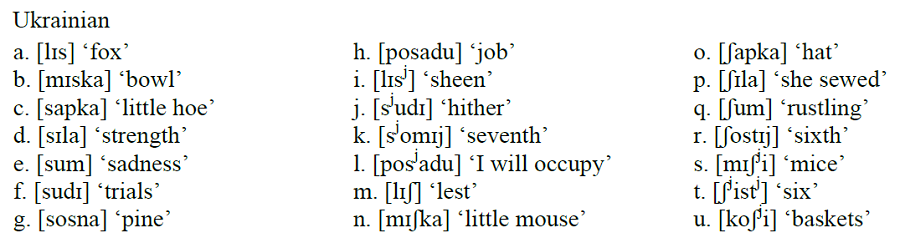
\includegraphics{../images/ukrainian.png}
\end{figure}

\newpage

{\large Question 5}\\

Topic: Phonological Relationships and Analysis\\
Source: Week 6 Handout, Question 11\\

What do the two signs below tell you about the phonological status of \underline{handshape} in ASL, and why?\\

\begin{figure}[H]
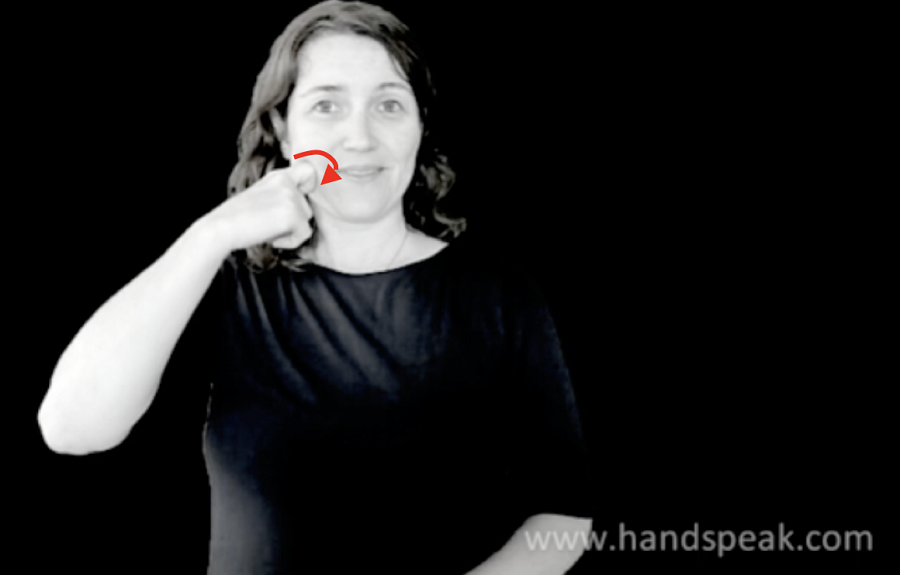
\includegraphics{../images/asl_apple.png}
\caption{APPLE}
\end{figure}
\begin{figure}[H]
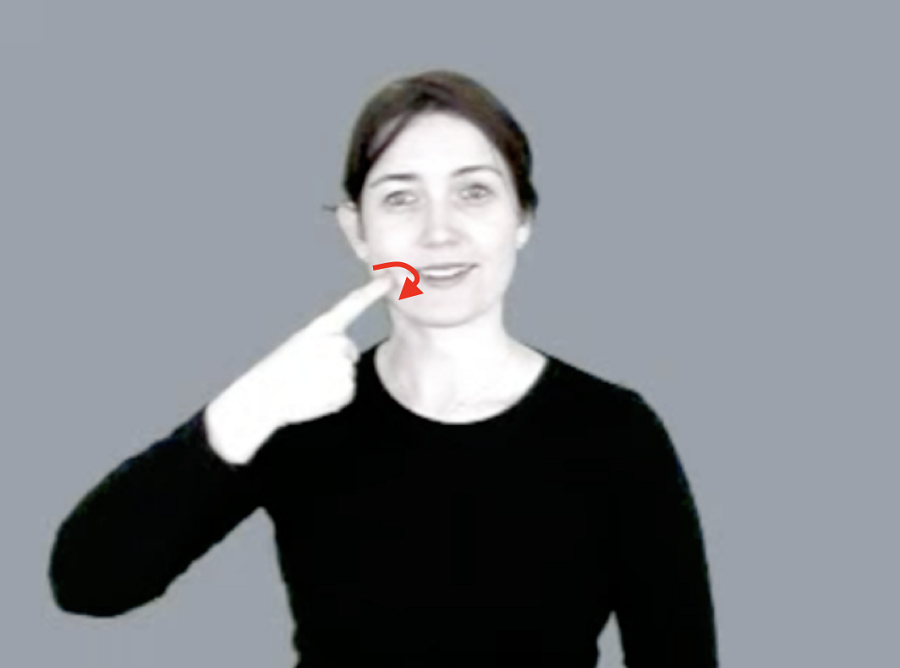
\includegraphics{../images/asl_candy.png}
\caption{CANDY}
\end{figure}

\newpage

\begin{center}
\textbf{{\color{red}{\HUGE END OF EXAM}}}\\

\end{center}
\newpage

\begin{center}
\textbf{{\color{blue}{\HUGE START OF EXAM\\}}}

\textbf{{\color{blue}{\HUGE Student ID: 17359\\}}}

\textbf{{\color{blue}{\HUGE \\}}}

\end{center}
\newpage

{\large Question 1}\\

Topic: Transcription\\
Source: Quiz 1, Question 10\\

Explain whether this word either does or does not have an [ʃ] sound in it, and why the spelling and pronunciation either do or do not align.\\

<bassoon>


\newpage

{\large Question 2}\\

Topic: Articulatory Phonetics\\
Source: Week 3 Discussion\\

Assuming a Standard North American English inventory, does this vowel need to have tenseness specified if you're giving a prose description? Why or why not?\\

{[ɑ]}


\newpage

{\large Question 3}\\

Topic: Phonological Features\\
Source: Quiz 3, Question 12\\

Explain how you figure out which feature is involved in the process of umlaut shown below.\\

\begin{figure}[H]
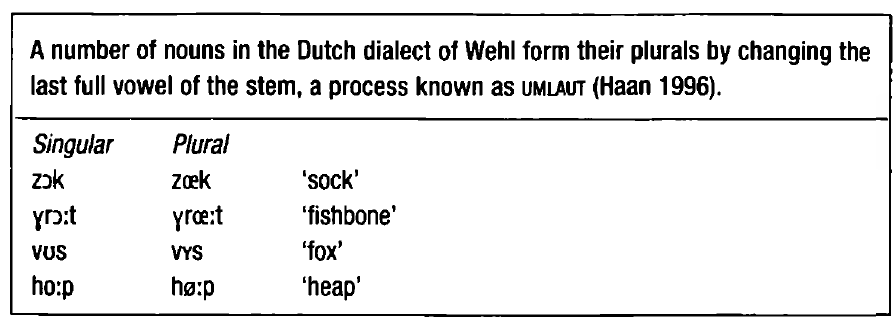
\includegraphics{../images/dutch.png}
\end{figure}

\newpage

{\large Question 4}\\

Topic: Skewed Distributions\\
Source: Week 5 Handout, Question 1\\

Explain why we think that languages are not random in terms of their phonology.\\


\newpage

{\large Question 5}\\

Topic: Phonological Relationships and Analysis\\
Source: Week 7 Handout, Question 12\\

What is the basic analysis of oral and nasal vowels in this dataset, and what are the key pieces of evidence?\\

\begin{figure}[H]
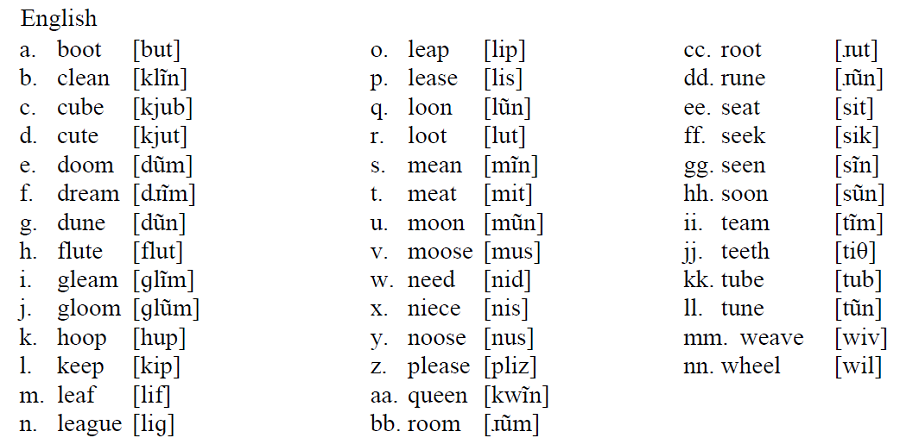
\includegraphics{../images/english12.png}
\end{figure}

\newpage

\begin{center}
\textbf{{\color{red}{\HUGE END OF EXAM}}}\\

\end{center}
\newpage

\begin{center}
\textbf{{\color{blue}{\HUGE START OF EXAM\\}}}

\textbf{{\color{blue}{\HUGE Student ID: 17393\\}}}

\textbf{{\color{blue}{\HUGE \\}}}

\end{center}
\newpage

{\large Question 1}\\

Topic: Transcription\\
Source: Week 2 Handout, Part II\\

Is this a reasonable transcription of this word? Explain why.\\

<mouse>: {[mɔɪs]}


\newpage

{\large Question 2}\\

Topic: Articulatory Phonetics\\
Source: Quiz 2, Question 6\\

In the pronunciation of this word, which sounds are obstruents and which are sonorants? Explain your answer.\\

<fricative>


\newpage

{\large Question 3}\\

Topic: Phonological Features\\
Source: Quiz 3, Question 3\\

Explain why this featural specification either does or does not match the given sound.\\

{[+consonantal]}, {[-sonorant]}

{[f]}


\newpage

{\large Question 4}\\

Topic: Skewed Distributions\\
Source: Week 5 Handout, Question 6\\

What would be a good description of the pattern in Malto? What characteristics make that a good description?\\

\begin{figure}[H]
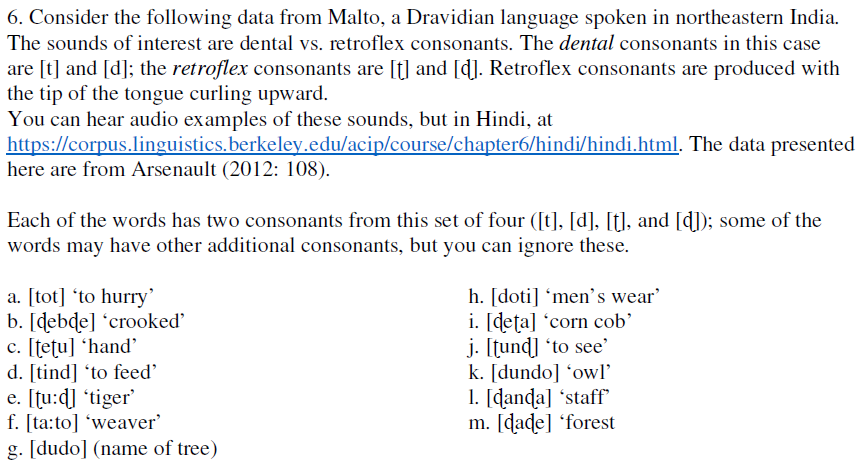
\includegraphics{../images/malto.png}
\end{figure}

\newpage

{\large Question 5}\\

Topic: Phonological Relationships and Analysis\\
Source: Week 6 Handout, Question 11\\

What do the two signs below tell you about the phonological status of \underline{handshape} in ASL, and why?\\

\begin{figure}[H]
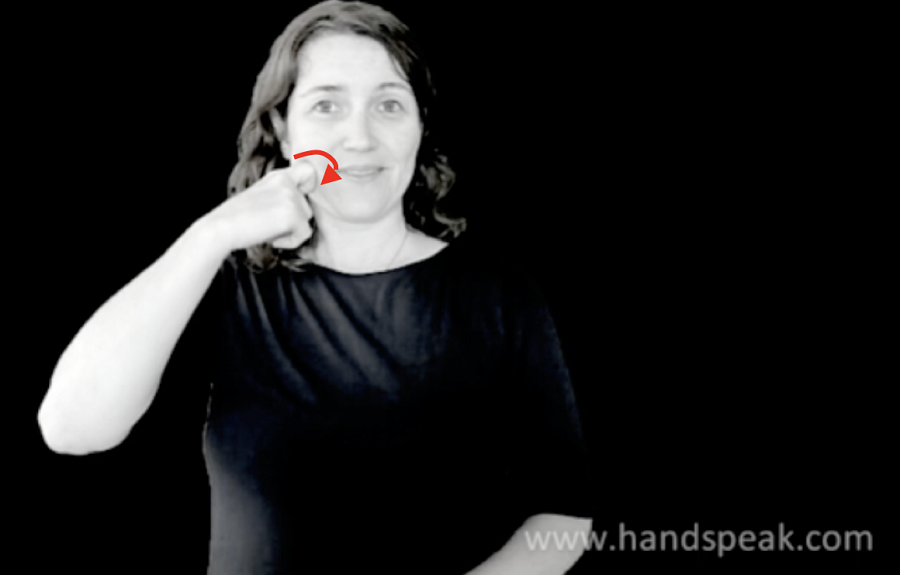
\includegraphics{../images/asl_apple.png}
\caption{APPLE}
\end{figure}
\begin{figure}[H]
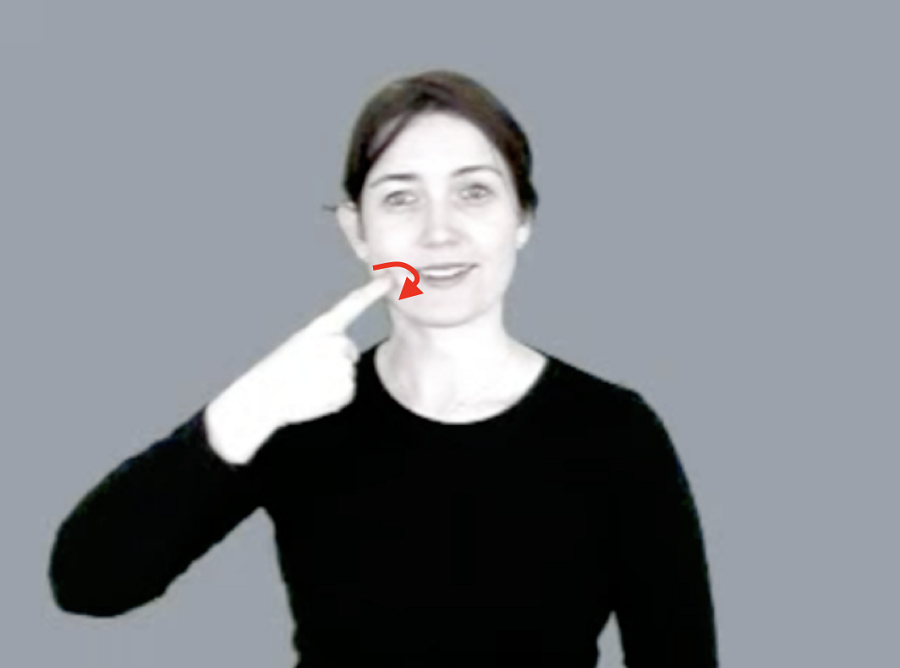
\includegraphics{../images/asl_candy.png}
\caption{CANDY}
\end{figure}

\newpage

\begin{center}
\textbf{{\color{red}{\HUGE END OF EXAM}}}\\

\end{center}
\newpage

\begin{center}
\textbf{{\color{blue}{\HUGE START OF EXAM\\}}}

\textbf{{\color{blue}{\HUGE Student ID: 17487\\}}}

\textbf{{\color{blue}{\HUGE \\}}}

\end{center}
\newpage

{\large Question 1}\\

Topic: Transcription\\
Source: Week 2 Handout, Part II, Question 3\\

Explain why people might legitimately disagree about how many sounds this particular word contains.\\

<better>


\newpage

{\large Question 2}\\

Topic: Articulatory Phonetics\\
Source: Week 3 Discussion\\

Describe what the tongue would do / where it would move during each of the vowels in this word.\\

<bookmark>


\newpage

{\large Question 3}\\

Topic: Phonological Features\\
Source: Week 4 Discussion\\

Explain what the given feature’s value is for this class of sounds, and why.\\

{[consonantal]}

glides


\newpage

{\large Question 4}\\

Topic: Skewed Distributions\\
Source: Week 5 Handout, Question 6\\

If I gave you a new word in Malto, [di\_\_u], would it be possible to predict whether it's [d] or [t] that goes in the blank? Explain why or why not.\\

\begin{figure}[H]
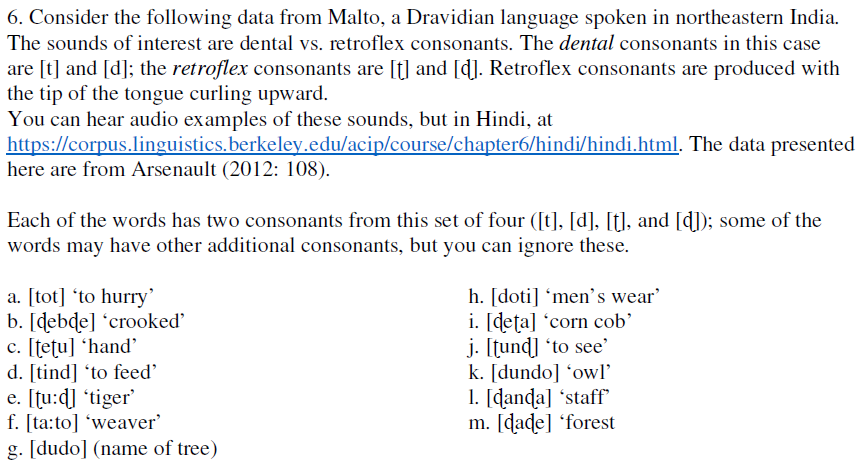
\includegraphics{../images/malto.png}
\end{figure}

\newpage

{\large Question 5}\\

Topic: Phonological Relationships and Analysis\\
Source: Week 6 Handout, Question 11\\

What do the two signs below tell you about the phonological status of \underline{handshape} in ASL, and why?\\

\begin{figure}[H]
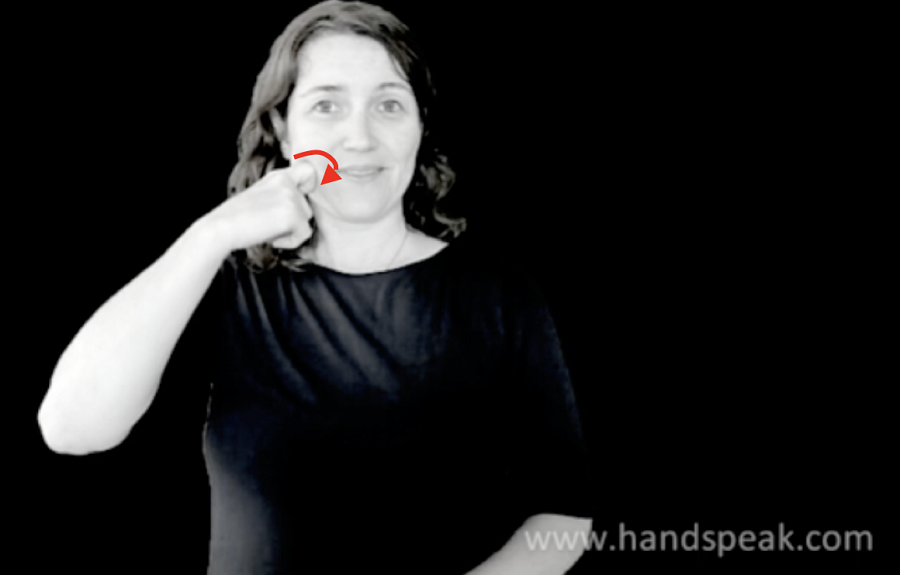
\includegraphics{../images/asl_apple.png}
\caption{APPLE}
\end{figure}
\begin{figure}[H]
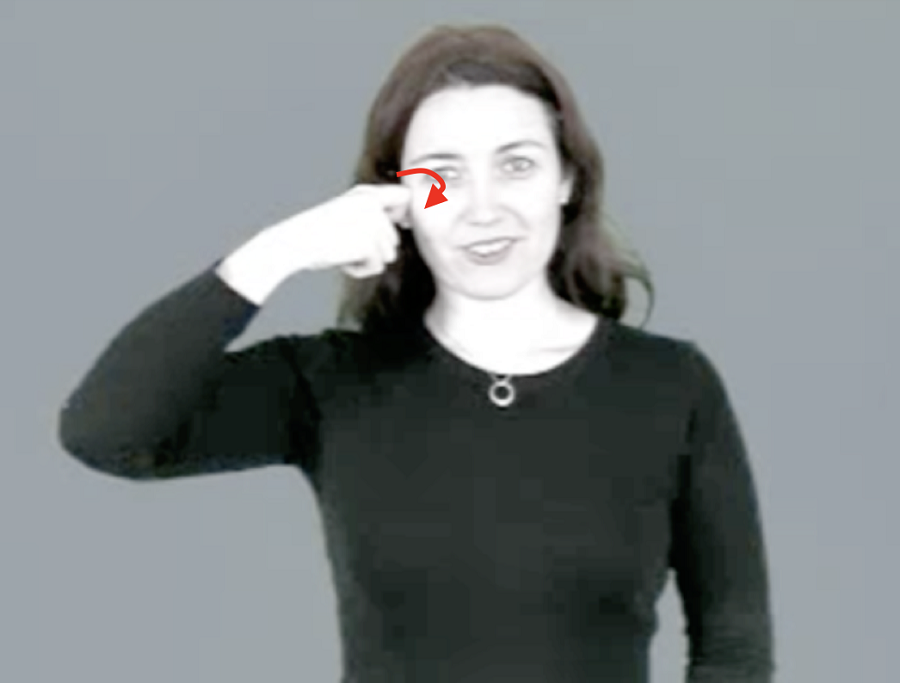
\includegraphics{../images/asl_onion.png}
\caption{ONION}
\end{figure}

\newpage

\begin{center}
\textbf{{\color{red}{\HUGE END OF EXAM}}}\\

\end{center}
\newpage

\begin{center}
\textbf{{\color{blue}{\HUGE START OF EXAM\\}}}

\textbf{{\color{blue}{\HUGE Student ID: 18870\\}}}

\textbf{{\color{blue}{\HUGE \\}}}

\end{center}
\newpage

{\large Question 1}\\

Topic: Transcription\\
Source: Week 2 Handout, Part II, Question 11\\

How would this word be transcribed?\\ (Kathleen will then ask a follow-up question about your transcription.)\\

<nice>


\newpage

{\large Question 2}\\

Topic: Articulatory Phonetics\\
Source: Week 3 Discussion\\

Describe what the tongue would do / where it would move during each of the vowels in this word.\\

<vacuum>


\newpage

{\large Question 3}\\

Topic: Phonological Features\\
Source: Week 4 Discussion\\

Explain what the given feature’s value is for this class of sounds, and why.\\

{[LABIAL]}

interdentals


\newpage

{\large Question 4}\\

Topic: Skewed Distributions\\
Source: Week 5 Handout, Question 6\\

If I gave you a new word in Malto, [di\_\_u], would it be possible to predict whether it's [d] or [ɖ] that goes in the blank? Explain why or why not.\\

\begin{figure}[H]
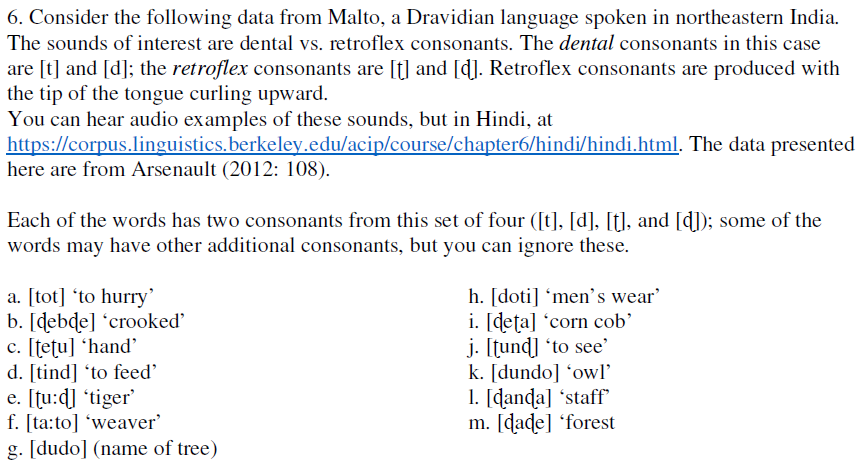
\includegraphics{../images/malto.png}
\end{figure}

\newpage

{\large Question 5}\\

Topic: Phonological Relationships and Analysis\\
Source: Week 6 Handout, Question 11\\

What do the two signs below tell you about the phonological status of \underline{handshape} in ASL, and why?\\

\begin{figure}[H]
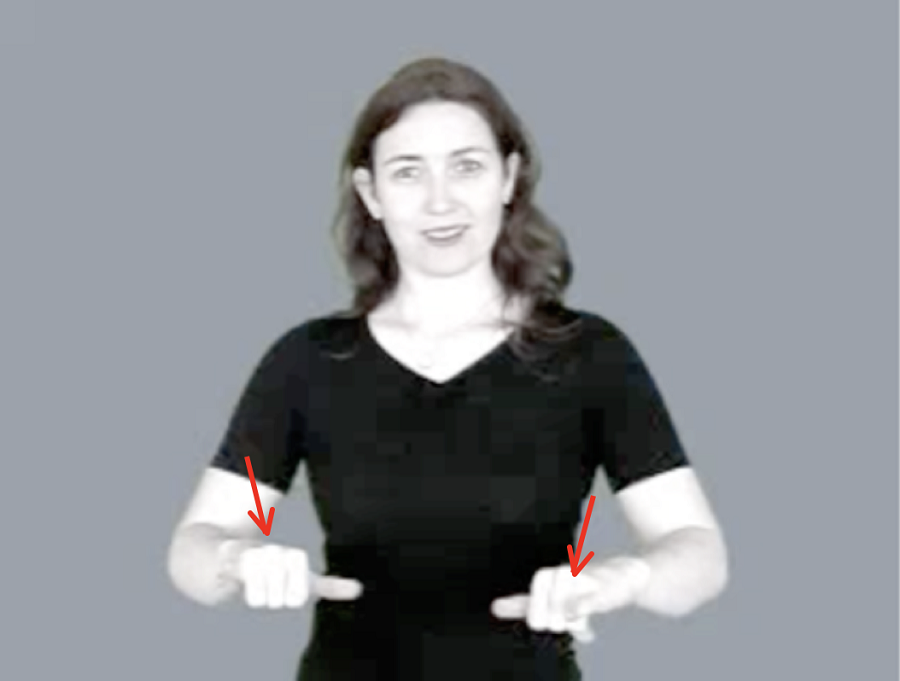
\includegraphics{../images/asl_stay.png}
\caption{STAY}
\end{figure}
\begin{figure}[H]
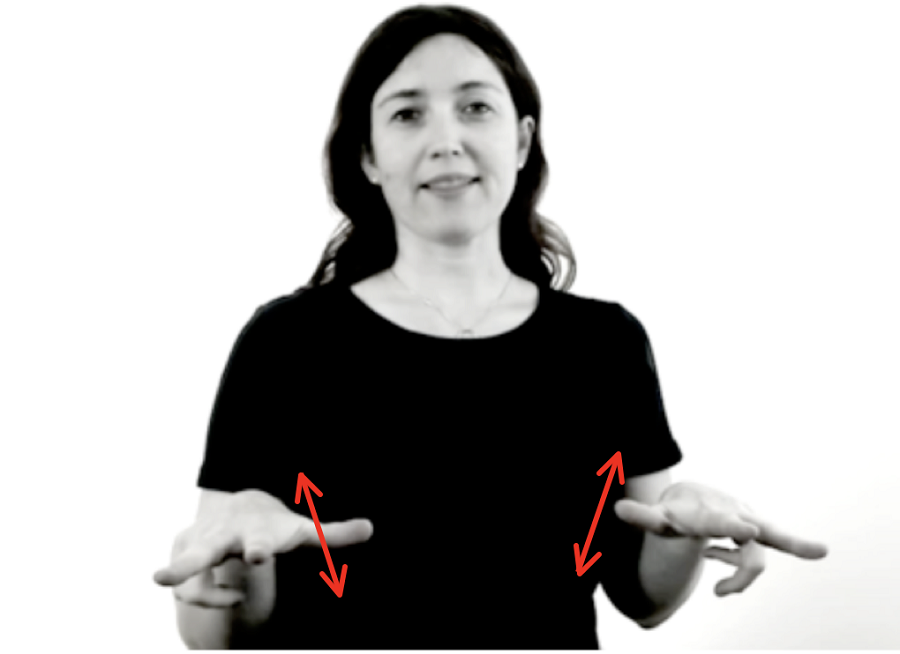
\includegraphics{../images/asl_awkward.png}
\caption{AWKWARD}
\end{figure}

\newpage

\begin{center}
\textbf{{\color{red}{\HUGE END OF EXAM}}}\\

\end{center}
\newpage

\begin{center}
\textbf{{\color{blue}{\HUGE START OF EXAM\\}}}

\textbf{{\color{blue}{\HUGE Student ID: 19086\\}}}

\textbf{{\color{blue}{\HUGE \\}}}

\end{center}
\newpage

{\large Question 1}\\

Topic: Transcription\\
Source: Week 2 Handout, Part II, Question 11\\

How would this word be transcribed?\\ (Kathleen will then ask a follow-up question about your transcription.)\\

<bird>


\newpage

{\large Question 2}\\

Topic: Articulatory Phonetics\\
Source: Homework 1, Question 3(a)\\

Could this image be the result of producing the sound represented by the given IPA symbol? Why or why not?\\

{[n]}

\begin{figure}[H]
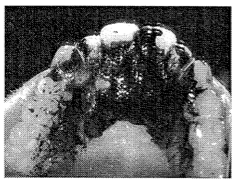
\includegraphics{../images/staticpalatography_stop.png}
\end{figure}

\newpage

{\large Question 3}\\

Topic: Phonological Features\\
Source: Week 4 Discussion\\

Explain why the given feature's value varies across this set of sounds.\\

{[voice]}

glottalized obstruents


\newpage

{\large Question 4}\\

Topic: Skewed Distributions\\
Source: Week 5 Handout, Question 6\\

What would be a good description of the pattern in Malto? What characteristics make that a good description?\\

\begin{figure}[H]
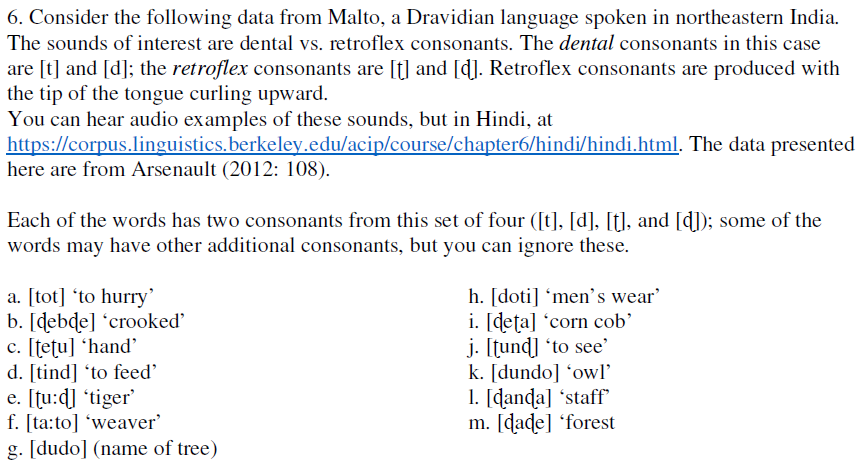
\includegraphics{../images/malto.png}
\end{figure}

\newpage

{\large Question 5}\\

Topic: Phonological Relationships and Analysis\\
Source: Week 7 Handout, Question 12\\

What is the basic analysis of oral and nasal vowels in this dataset, and what are the key pieces of evidence?\\

\begin{figure}[H]
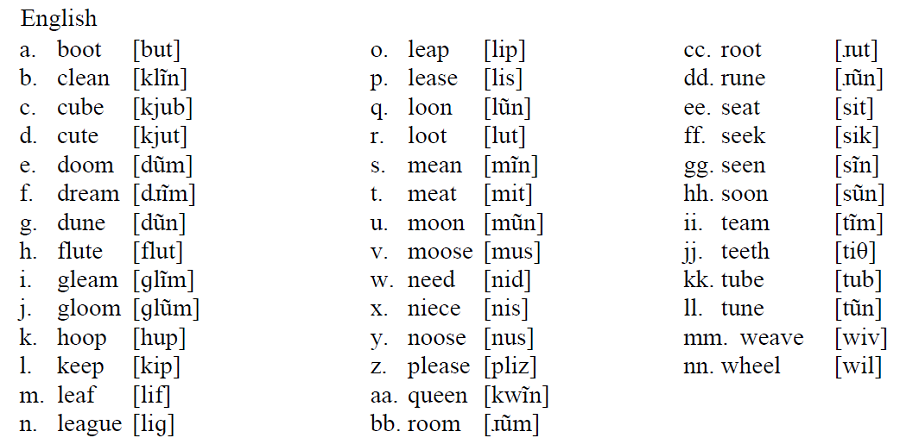
\includegraphics{../images/english12.png}
\end{figure}

\newpage

\begin{center}
\textbf{{\color{red}{\HUGE END OF EXAM}}}\\

\end{center}
\newpage

\begin{center}
\textbf{{\color{blue}{\HUGE START OF EXAM\\}}}

\textbf{{\color{blue}{\HUGE Student ID: 19711\\}}}

\textbf{{\color{blue}{\HUGE \\}}}

\end{center}
\newpage

{\large Question 1}\\

Topic: Transcription\\
Source: Week 2 Handout, Part II\\

Is this a reasonable transcription of this word? Explain why.\\

<wimp>: {[wimp]}


\newpage

{\large Question 2}\\

Topic: Articulatory Phonetics\\
Source: Week 3 Discussion\\

Describe what the tongue would do / where it would move during each of the vowels in this word.\\

<puny>


\newpage

{\large Question 3}\\

Topic: Phonological Features\\
Source: Week 4 Discussion\\

Explain what the given feature’s value is for this class of sounds, and why.\\

{[continuant]}

glottals


\newpage

{\large Question 4}\\

Topic: Skewed Distributions\\
Source: Week 5 Handout, Question 6\\

What would be a good description of the pattern in Malto? What characteristics make that a good description?\\

\begin{figure}[H]
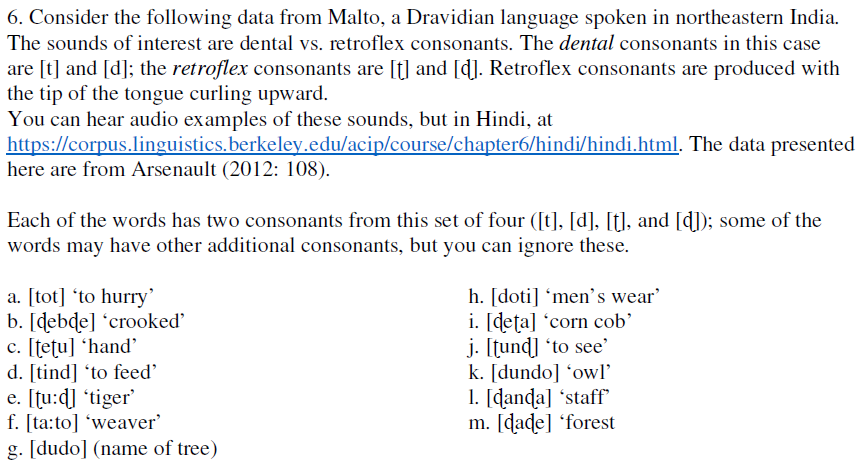
\includegraphics{../images/malto.png}
\end{figure}

\newpage

{\large Question 5}\\

Topic: Phonological Relationships and Analysis\\
Source: Week 6 Handout, Question 11\\

What do the two signs below tell you about the phonological status of \underline{handshape} in ASL, and why?\\

\begin{figure}[H]
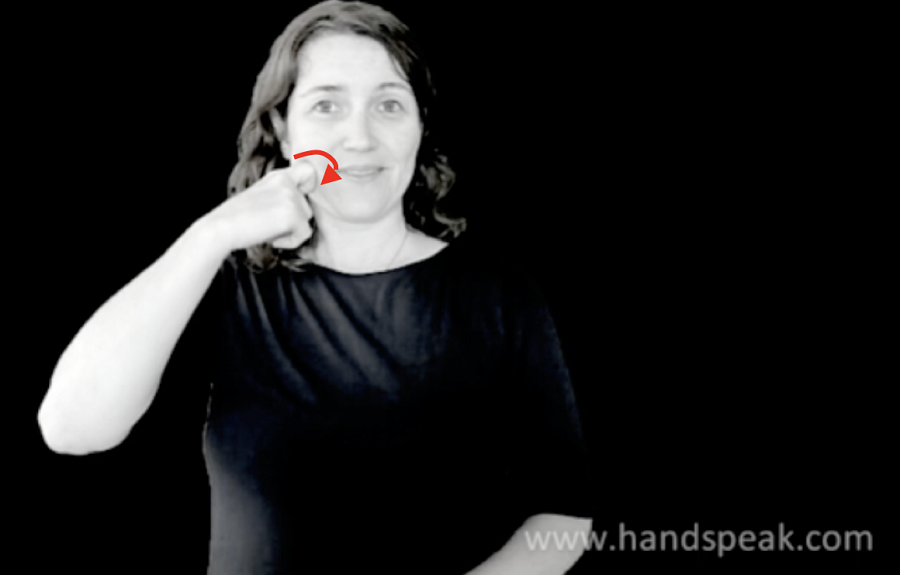
\includegraphics{../images/asl_apple.png}
\caption{APPLE}
\end{figure}
\begin{figure}[H]
\includegraphics{../images/asl_onion.png}
\caption{ONION}
\end{figure}

\newpage

\begin{center}
\textbf{{\color{red}{\HUGE END OF EXAM}}}\\

\end{center}
\newpage

\begin{center}
\textbf{{\color{blue}{\HUGE START OF EXAM\\}}}

\textbf{{\color{blue}{\HUGE Student ID: 20054\\}}}

\textbf{{\color{blue}{\HUGE \\}}}

\end{center}
\newpage

{\large Question 1}\\

Topic: Transcription\\
Source: Week 2 Handout, Part II, Question 11\\

How would this word be transcribed?\\ (Kathleen will then ask a follow-up question about your transcription.)\\

<frog>


\newpage

{\large Question 2}\\

Topic: Articulatory Phonetics\\
Source: Week 3 Discussion\\

Describe what the tongue would do / where it would move during each of the vowels in this word.\\

<puny>


\newpage

{\large Question 3}\\

Topic: Phonological Features\\
Source: Quiz 3, Question 12\\

Explain how you figure out which feature is involved in the process of umlaut shown below.\\

\begin{figure}[H]
\includegraphics{../images/dutch.png}
\end{figure}

\newpage

{\large Question 4}\\

Topic: Skewed Distributions\\
Source: Week 5 Handout, Question 3\\

What evidence is there that there is a pattern in these data, assuming that these are the only CV and VC sequences that occur in some language?\\

{[sa]}, {[ʃi]}, {[za]}, {[ʒi]}, {[as]}, {[iʃ]}, {[az]}, {[iʒ]}


\newpage

{\large Question 5}\\

Topic: Phonological Relationships and Analysis\\
Source: Week 6 Handout, Question 11\\

What do the two signs below tell you about the phonological status of \underline{handshape} in ASL, and why?\\

\begin{figure}[H]
\includegraphics{../images/asl_apple.png}
\caption{APPLE}
\end{figure}
\begin{figure}[H]
\includegraphics{../images/asl_now.png}
\caption{NOW}
\end{figure}

\newpage

\begin{center}
\textbf{{\color{red}{\HUGE END OF EXAM}}}\\

\end{center}
\newpage

\begin{center}
\textbf{{\color{blue}{\HUGE START OF EXAM\\}}}

\textbf{{\color{blue}{\HUGE Student ID: 22413\\}}}

\textbf{{\color{blue}{\HUGE \\}}}

\end{center}
\newpage

{\large Question 1}\\

Topic: Transcription\\
Source: Week 2 Handout, Part II, Question 11\\

How would this word be transcribed?\\ (Kathleen will then ask a follow-up question about your transcription.)\\

<segment>


\newpage

{\large Question 2}\\

Topic: Articulatory Phonetics\\
Source: Week 3 Handout, Question 7\\

Is the symbol given a reasonable way to transcribe any of the sounds described below? If so, which one? If not, why not? Explain your answer.\\

{[v]}

\begin{itemize} \item voiceless palatal affricate \item voiced velar nasal \item voiceless glottal fricative \item voiced labiodental fricative \item voiced interdental fricative \item voiced palatal fricative \end{itemize}


\newpage

{\large Question 3}\\

Topic: Phonological Features\\
Source: Week 4 Discussion\\

Explain what the given feature’s value is for this class of sounds, and why.\\

{[approximant]}

nasals


\newpage

{\large Question 4}\\

Topic: Skewed Distributions\\
Source: Week 5 Handout, Question 5\\

Explain why looking for patterns with consonants and vowels is a more reasonable approach to pattern finding in this dataset than looking for patterns with respect to all of the individual sounds in Ukrainian.\\

\begin{figure}[H]
\includegraphics{../images/ukrainian.png}
\end{figure}

\newpage

{\large Question 5}\\

Topic: Phonological Relationships and Analysis\\
Source: Week 6 Handout, Question 11\\

What do the two signs below tell you about the phonological status of \underline{handshape} in ASL, and why?\\

\begin{figure}[H]
\includegraphics{../images/asl_stay.png}
\caption{STAY}
\end{figure}
\begin{figure}[H]
\includegraphics{../images/asl_awkward.png}
\caption{AWKWARD}
\end{figure}

\newpage

\begin{center}
\textbf{{\color{red}{\HUGE END OF EXAM}}}\\

\end{center}
\newpage

\begin{center}
\textbf{{\color{blue}{\HUGE START OF EXAM\\}}}

\textbf{{\color{blue}{\HUGE Student ID: 23000\\}}}

\textbf{{\color{blue}{\HUGE \\}}}

\end{center}
\newpage

{\large Question 1}\\

Topic: Transcription\\
Source: Week 2 Handout, Part II\\

Is this a reasonable transcription of this word? Explain why.\\

<shows>: {[ʃoʊs]}


\newpage

{\large Question 2}\\

Topic: Articulatory Phonetics\\
Source: Homework 1, Question 3(b)\\

Explain why this is or is not a complete phonetic natural class in standard North American English.\\

{[f]}, {[s]}, {[ʃ]}


\newpage

{\large Question 3}\\

Topic: Phonological Features\\
Source: Quiz 3, Question 3\\

Explain why this featural specification either does or does not match the given sound.\\

{[-consonantal]}, {[-sonorant]}

{[u]}


\newpage

{\large Question 4}\\

Topic: Skewed Distributions\\
Source: Week 5 Handout, Question 1\\

Explain why we think that languages are not random in terms of their phonology.\\


\newpage

{\large Question 5}\\

Topic: Phonological Relationships and Analysis\\
Source: Week 6 Handout, Question 11\\

What do the two signs below tell you about the phonological status of \underline{handshape} in ASL, and why?\\

\begin{figure}[H]
\includegraphics{../images/asl_apple.png}
\caption{APPLE}
\end{figure}
\begin{figure}[H]
\includegraphics{../images/asl_now.png}
\caption{NOW}
\end{figure}

\newpage

\begin{center}
\textbf{{\color{red}{\HUGE END OF EXAM}}}\\

\end{center}
\newpage

\begin{center}
\textbf{{\color{blue}{\HUGE START OF EXAM\\}}}

\textbf{{\color{blue}{\HUGE Student ID: 23071\\}}}

\textbf{{\color{blue}{\HUGE \\}}}

\end{center}
\newpage

{\large Question 1}\\

Topic: Transcription\\
Source: Week 2 Handout, Part II, Question 11\\

How would this word be transcribed?\\ (Kathleen will then ask a follow-up question about your transcription.)\\

<finger>


\newpage

{\large Question 2}\\

Topic: Articulatory Phonetics\\
Source: Week 2 Handout, Part I, Question 12\\

Explain in what sense the difference between the sounds in the words <but> and <cut> is SIMILAR to and also DIFFERENT from the difference between the sounds in the words <bit> and <kit>.\\


\newpage

{\large Question 3}\\

Topic: Phonological Features\\
Source: Week 4 Discussion\\

Explain what the given feature’s value is for this class of sounds, and why.\\

{[continuant]}

glottals


\newpage

{\large Question 4}\\

Topic: Skewed Distributions\\
Source: Week 5 Handout, Question 7\\

Explain how you would go about looking for co-occurrence restrictions in bi-syllabic signs in ASL. (Refer to the data that follows.)\\

\begin{figure}[H]
\includegraphics{../images/ASL_movement.png}
\end{figure}

\newpage

{\large Question 5}\\

Topic: Phonological Relationships and Analysis\\
Source: Week 7 Handout, Question 9\\

What is the basic analysis of vowel length in this dataset, and what are the key pieces of evidence?\\

\begin{figure}[H]
\includegraphics{../images/malayalam.png}
\end{figure}

\newpage

\begin{center}
\textbf{{\color{red}{\HUGE END OF EXAM}}}\\

\end{center}
\newpage

\begin{center}
\textbf{{\color{blue}{\HUGE START OF EXAM\\}}}

\textbf{{\color{blue}{\HUGE Student ID: 23100\\}}}

\textbf{{\color{blue}{\HUGE \\}}}

\end{center}
\newpage

{\large Question 1}\\

Topic: Transcription\\
Source: Week 2 Handout, Part II\\

Is this a reasonable transcription of this word? Explain why.\\

<mine>: {[mɑɪn]}


\newpage

{\large Question 2}\\

Topic: Articulatory Phonetics\\
Source: Week 3 Discussion\\

Assuming a Standard North American English inventory, does this vowel need to have tenseness specified if you're giving a prose description? Why or why not?\\

{[ɛ]}


\newpage

{\large Question 3}\\

Topic: Phonological Features\\
Source: Homework 2, Question 1\\

Explain which sound should be removed to make this a natural class (assuming SNAE, except that there are no diphthongs, no [ə] or [ʌ], no syllabic consonants, and no [w̥]), and what the minimum set of features would be to describe the resulting natural class.\\

{[b]}, {[d]}, {[z]}, {[ɾ]}, {[n]}, {[l]}, {[ɹ]}


\newpage

{\large Question 4}\\

Topic: Skewed Distributions\\
Source: Week 5 Handout, Question 5\\

Explain why it is possible to predict which of [s] or [ʃʲ] will occur in a new environment in Ukrainian, but not possible to predict which of [s] or [ʃ] will occur in a new environment.\\

\begin{figure}[H]
\includegraphics{../images/ukrainian.png}
\end{figure}

\newpage

{\large Question 5}\\

Topic: Phonological Relationships and Analysis\\
Source: Week 6 Handout, Question 11\\

What do the two signs below tell you about the phonological status of \underline{handshape} in ASL, and why?\\

\begin{figure}[H]
\includegraphics{../images/asl_apple.png}
\caption{APPLE}
\end{figure}
\begin{figure}[H]
\includegraphics{../images/asl_candy.png}
\caption{CANDY}
\end{figure}

\newpage

\begin{center}
\textbf{{\color{red}{\HUGE END OF EXAM}}}\\

\end{center}
\newpage

\begin{center}
\textbf{{\color{blue}{\HUGE START OF EXAM\\}}}

\textbf{{\color{blue}{\HUGE Student ID: 23286\\}}}

\textbf{{\color{blue}{\HUGE \\}}}

\end{center}
\newpage

{\large Question 1}\\

Topic: Transcription\\
Source: Week 2 Handout, Part II, Question 11\\

How would this word be transcribed?\\ (Kathleen will then ask a follow-up question about your transcription.)\\

<finger>


\newpage

{\large Question 2}\\

Topic: Articulatory Phonetics\\
Source: Week 3 Handout, Question 3\\

Explain why the additional vowel below either does or does not belong in the phonetic natural class defined by the original set of SNAE vowels.\\

Original set: {[ɛ]}, {[ɪ]}, {[ʊ]}, {[ɔ]}

Addition: {[ɑ]}


\newpage

{\large Question 3}\\

Topic: Phonological Features\\
Source: Week 4 Discussion\\

Explain what the given feature’s value is for this class of sounds, and why.\\

{[LABIAL]}

interdentals


\newpage

{\large Question 4}\\

Topic: Skewed Distributions\\
Source: Week 5 Handout, Question 5\\

Explain why it is possible to predict which of [s] or [ʃʲ] will occur in a new environment in Ukrainian, but not possible to predict which of [s] or [ʃ] will occur in a new environment.\\

\begin{figure}[H]
\includegraphics{../images/ukrainian.png}
\end{figure}

\newpage

{\large Question 5}\\

Topic: Phonological Relationships and Analysis\\
Source: Week 7 Handout, Question 12\\

What is the basic analysis of oral and nasal vowels in this dataset, and what are the key pieces of evidence?\\

\begin{figure}[H]
\includegraphics{../images/english12.png}
\end{figure}

\newpage

\begin{center}
\textbf{{\color{red}{\HUGE END OF EXAM}}}\\

\end{center}
\newpage

\begin{center}
\textbf{{\color{blue}{\HUGE START OF EXAM\\}}}

\textbf{{\color{blue}{\HUGE Student ID: 24476\\}}}

\textbf{{\color{blue}{\HUGE \\}}}

\end{center}
\newpage

{\large Question 1}\\

Topic: Transcription\\
Source: Week 2 Handout, Part II, Question 11\\

How would this word be transcribed?\\ (Kathleen will then ask a follow-up question about your transcription.)\\

<wealth>


\newpage

{\large Question 2}\\

Topic: Articulatory Phonetics\\
Source: Week 3 Handout, Question 7\\

Is the symbol given a reasonable way to transcribe any of the sounds described below? If so, which one? If not, why not? Explain your answer.\\

{[ʒ]}

\begin{itemize} \item voiceless palatal affricate \item voiced velar nasal \item voiceless glottal fricative \item voiced labiodental fricative \item voiced interdental fricative \item voiced palatal fricative \end{itemize}


\newpage

{\large Question 3}\\

Topic: Phonological Features\\
Source: Homework 2, Question 1\\

Explain which sound should be removed to make this a natural class (assuming SNAE, except that there are no diphthongs, no [ə] or [ʌ], no syllabic consonants, and no [w̥]), and what the minimum set of features would be to describe the resulting natural class.\\

{[b]}, {[d]}, {[z]}, {[ɾ]}, {[n]}, {[l]}, {[ɹ]}


\newpage

{\large Question 4}\\

Topic: Skewed Distributions\\
Source: Week 5 Handout, Question 7\\

Explain how you would go about looking for co-occurrence restrictions in bi-syllabic signs in ASL. (Refer to the data that follows.)\\

\begin{figure}[H]
\includegraphics{../images/ASL_movement.png}
\end{figure}

\newpage

{\large Question 5}\\

Topic: Phonological Relationships and Analysis\\
Source: Week 7 Handout, Question 9\\

What is the basic analysis of vowel length in this dataset, and what are the key pieces of evidence?\\

\begin{figure}[H]
\includegraphics{../images/malayalam.png}
\end{figure}

\newpage

\begin{center}
\textbf{{\color{red}{\HUGE END OF EXAM}}}\\

\end{center}
\newpage

\begin{center}
\textbf{{\color{blue}{\HUGE START OF EXAM\\}}}

\textbf{{\color{blue}{\HUGE Student ID: 27121\\}}}

\textbf{{\color{blue}{\HUGE \\}}}

\end{center}
\newpage

{\large Question 1}\\

Topic: Transcription\\
Source: Week 2 Handout, Part II, Question 11\\

How would this word be transcribed?\\ (Kathleen will then ask a follow-up question about your transcription.)\\

<segment>


\newpage

{\large Question 2}\\

Topic: Articulatory Phonetics\\
Source: Week 3 Discussion\\

Describe what the tongue would do / where it would move during each of the vowels in this word.\\

<follow>


\newpage

{\large Question 3}\\

Topic: Phonological Features\\
Source: Week 4 Discussion\\

Explain what the given feature’s value is for this class of sounds, and why.\\

{[consonantal]}

glides


\newpage

{\large Question 4}\\

Topic: Skewed Distributions\\
Source: Week 5 Handout, Question 6\\

If I gave you a new word in Malto, [di\_\_u], would it be possible to predict whether it's [d] or [ɖ] that goes in the blank? Explain why or why not.\\

\begin{figure}[H]
\includegraphics{../images/malto.png}
\end{figure}

\newpage

{\large Question 5}\\

Topic: Phonological Relationships and Analysis\\
Source: Week 6 Handout, Question 11\\

What do the two signs below tell you about the phonological status of \underline{handshape} in ASL, and why?\\

\begin{figure}[H]
\includegraphics{../images/asl_apple.png}
\caption{APPLE}
\end{figure}
\begin{figure}[H]
\includegraphics{../images/asl_onion.png}
\caption{ONION}
\end{figure}

\newpage

\begin{center}
\textbf{{\color{red}{\HUGE END OF EXAM}}}\\

\end{center}
\newpage

\begin{center}
\textbf{{\color{blue}{\HUGE START OF EXAM\\}}}

\textbf{{\color{blue}{\HUGE Student ID: 27762\\}}}

\textbf{{\color{blue}{\HUGE \\}}}

\end{center}
\newpage

{\large Question 1}\\

Topic: Transcription\\
Source: Week 2 Handout, Part II, Question 11\\

How would this word be transcribed?\\ (Kathleen will then ask a follow-up question about your transcription.)\\

<cough>


\newpage

{\large Question 2}\\

Topic: Articulatory Phonetics\\
Source: Week 3 Handout, Question 7\\

Is the symbol given a reasonable way to transcribe any of the sounds described below? If so, which one? If not, why not? Explain your answer.\\

{[ʒ]}

\begin{itemize} \item voiceless palatal affricate \item voiced velar nasal \item voiceless glottal fricative \item voiced labiodental fricative \item voiced interdental fricative \item voiced palatal fricative \end{itemize}


\newpage

{\large Question 3}\\

Topic: Phonological Features\\
Source: Homework 2, Question 1\\

Explain which sound should be removed to make this a natural class (assuming SNAE, except that there are no diphthongs, no [ə] or [ʌ], no syllabic consonants, and no [w̥]), and what the minimum set of features would be to describe the resulting natural class.\\

{[i]}, {[ɪ]}, {[e]}, {[ɛ]}, {[æ]}, {[ɑ]}, {[ɔ]}, {[o]}, {[ʊ]}, {[u]}, {[ʒ]}, {[k]}, {[ɡ]}, {[ŋ]}, {[w]}


\newpage

{\large Question 4}\\

Topic: Skewed Distributions\\
Source: Week 5 Handout, Question 5\\

Explain why looking for patterns with consonants and vowels is a more reasonable approach to pattern finding in this dataset than looking for patterns with respect to all of the individual sounds in Ukrainian.\\

\begin{figure}[H]
\includegraphics{../images/ukrainian.png}
\end{figure}

\newpage

{\large Question 5}\\

Topic: Phonological Relationships and Analysis\\
Source: Week 7 Handout, Question 12\\

What is the basic analysis of oral and nasal vowels in this dataset, and what are the key pieces of evidence?\\

\begin{figure}[H]
\includegraphics{../images/english12.png}
\end{figure}

\newpage

\begin{center}
\textbf{{\color{red}{\HUGE END OF EXAM}}}\\

\end{center}
\newpage

\begin{center}
\textbf{{\color{blue}{\HUGE START OF EXAM\\}}}

\textbf{{\color{blue}{\HUGE Student ID: 28926\\}}}

\textbf{{\color{blue}{\HUGE \\}}}

\end{center}
\newpage

{\large Question 1}\\

Topic: Transcription\\
Source: Week 2 Handout, Part II, Question 11\\

How would this word be transcribed?\\ (Kathleen will then ask a follow-up question about your transcription.)\\

<goat>


\newpage

{\large Question 2}\\

Topic: Articulatory Phonetics\\
Source: Week 3 Discussion\\

Assuming a Standard North American English inventory, does this vowel need to have tenseness specified if you're giving a prose description? Why or why not?\\

{[u]}


\newpage

{\large Question 3}\\

Topic: Phonological Features\\
Source: Week 4 Discussion\\

Explain why phonological features are used instead of phonetic characteristics in analyzing datasets.\\


\newpage

{\large Question 4}\\

Topic: Skewed Distributions\\
Source: Week 5 Handout, Question 2\\

Explain why there should only be 8 sequences listed in the answer, even though multiplying 4 x 4 would give you 16 possible sequences.\\

\begin{figure}[H]
\includegraphics{../images/skew2.png}
\end{figure}

\newpage

{\large Question 5}\\

Topic: Phonological Relationships and Analysis\\
Source: Week 7 Handout, Question 9\\

What is the basic analysis of vowel length in this dataset, and what are the key pieces of evidence?\\

\begin{figure}[H]
\includegraphics{../images/malayalam.png}
\end{figure}

\newpage

\begin{center}
\textbf{{\color{red}{\HUGE END OF EXAM}}}\\

\end{center}
\newpage

\begin{center}
\textbf{{\color{blue}{\HUGE START OF EXAM\\}}}

\textbf{{\color{blue}{\HUGE Student ID: 29164\\}}}

\textbf{{\color{blue}{\HUGE \\}}}

\end{center}
\newpage

{\large Question 1}\\

Topic: Transcription\\
Source: Week 2 Handout, Part II\\

Is this a reasonable transcription of this word? Explain why.\\

<paid>: {[peid]}


\newpage

{\large Question 2}\\

Topic: Articulatory Phonetics\\
Source: Week 3 Handout, Question 7\\

Is the symbol given a reasonable way to transcribe any of the sounds described below? If so, which one? If not, why not? Explain your answer.\\

{[ʒ]}

\begin{itemize} \item voiceless palatal affricate \item voiced velar nasal \item voiceless glottal fricative \item voiced labiodental fricative \item voiced interdental fricative \item voiced palatal fricative \end{itemize}


\newpage

{\large Question 3}\\

Topic: Phonological Features\\
Source: Homework 2, Question 1\\

Explain which sound should be removed to make this a natural class (assuming SNAE, except that there are no diphthongs, no [ə] or [ʌ], no syllabic consonants, and no [w̥]), and what the minimum set of features would be to describe the resulting natural class.\\

{[i]}, {[ɪ]}, {[ɛ]}, {[u]}, {[ʊ]}


\newpage

{\large Question 4}\\

Topic: Skewed Distributions\\
Source: Week 5 Handout, Question 1\\

Explain why we think that languages are not random in terms of their phonology.\\


\newpage

{\large Question 5}\\

Topic: Phonological Relationships and Analysis\\
Source: Week 6 Handout, Question 11\\

What do the two signs below tell you about the phonological status of \underline{handshape} in ASL, and why?\\

\begin{figure}[H]
\includegraphics{../images/asl_apple.png}
\caption{APPLE}
\end{figure}
\begin{figure}[H]
\includegraphics{../images/asl_candy.png}
\caption{CANDY}
\end{figure}

\newpage

\begin{center}
\textbf{{\color{red}{\HUGE END OF EXAM}}}\\

\end{center}
\newpage

\begin{center}
\textbf{{\color{blue}{\HUGE START OF EXAM\\}}}

\textbf{{\color{blue}{\HUGE Student ID: 30263\\}}}

\textbf{{\color{blue}{\HUGE \\}}}

\end{center}
\newpage

{\large Question 1}\\

Topic: Transcription\\
Source: Week 2 Handout, Part II, Question 3\\

Explain why people might legitimately disagree about how many sounds this particular word contains.\\

<rice>


\newpage

{\large Question 2}\\

Topic: Articulatory Phonetics\\
Source: Week 3 Handout, Question 3\\

Explain why the additional vowel below either does or does not belong in the phonetic natural class defined by the original set of SNAE vowels.\\

Original set: {[ɛ]}, {[ɪ]}, {[ʊ]}, {[ɔ]}

Addition: {[ɑ]}


\newpage

{\large Question 3}\\

Topic: Phonological Features\\
Source: Homework 2, Question 1\\

Explain which sound should be removed to make this a natural class (assuming SNAE, except that there are no diphthongs, no [ə] or [ʌ], no syllabic consonants, and no [w̥]), and what the minimum set of features would be to describe the resulting natural class.\\

{[b]}, {[d]}, {[z]}, {[ɾ]}, {[n]}, {[l]}, {[ɹ]}


\newpage

{\large Question 4}\\

Topic: Skewed Distributions\\
Source: Week 5 Handout, Question 1\\

Explain why we think that languages are not random in terms of their phonology.\\


\newpage

{\large Question 5}\\

Topic: Phonological Relationships and Analysis\\
Source: Week 6 Handout, Question 11\\

What do the two signs below tell you about the phonological status of \underline{handshape} in ASL, and why?\\

\begin{figure}[H]
\includegraphics{../images/asl_apple.png}
\caption{APPLE}
\end{figure}
\begin{figure}[H]
\includegraphics{../images/asl_onion.png}
\caption{ONION}
\end{figure}

\newpage

\begin{center}
\textbf{{\color{red}{\HUGE END OF EXAM}}}\\

\end{center}
\newpage

\begin{center}
\textbf{{\color{blue}{\HUGE START OF EXAM\\}}}

\textbf{{\color{blue}{\HUGE Student ID: 30511\\}}}

\textbf{{\color{blue}{\HUGE \\}}}

\end{center}
\newpage

{\large Question 1}\\

Topic: Transcription\\
Source: Quiz 1, Question 10\\

Explain whether this word either does or does not have an [ʃ] sound in it, and why the spelling and pronunciation either do or do not align.\\

<mishandle>


\newpage

{\large Question 2}\\

Topic: Articulatory Phonetics\\
Source: Week 3 Handout, Question 13\\

Explain why this image does or does not match the description.\\

\begin{itemize} \item A one-handed sign. \item Location: At the signer’s nose. \item Handshape: Starts with index finger extended; finger folds down into a “hook” shape during the sign; then straightens and repeats the folding. \item Movement: No movement other than the change in handshape. \end{itemize}

\begin{figure}[H]
\includegraphics{../images/taiwansign_wrong.png}
\caption{WRONG}
\end{figure}

\newpage

{\large Question 3}\\

Topic: Phonological Features\\
Source: Quiz 3, Question 12\\

Explain how you figure out which feature is involved in the process of umlaut shown below.\\

\begin{figure}[H]
\includegraphics{../images/dutch.png}
\end{figure}

\newpage

{\large Question 4}\\

Topic: Skewed Distributions\\
Source: Quiz 4, Question 2\\

L$_X$ (Language X) has three vowels, [i], [a], and [u]. L$_X$ has tri-syllabic roots. If L$_X$ does not allow non-identical high vowels to co-occur, which one of the following tri-syllabic vocalic sequences do you predict to be unattested in L$_X$? Explain why.\\

\begin{itemize} \item {[u...i...a]} \item {[a...i...a]} \item {[u...u...a]} \item {[a...i...i]} \end{itemize}


\newpage

{\large Question 5}\\

Topic: Phonological Relationships and Analysis\\
Source: Week 7 Handout, Question 12\\

What is the basic analysis of oral and nasal vowels in this dataset, and what are the key pieces of evidence?\\

\begin{figure}[H]
\includegraphics{../images/english12.png}
\end{figure}

\newpage

\begin{center}
\textbf{{\color{red}{\HUGE END OF EXAM}}}\\

\end{center}
\newpage

\begin{center}
\textbf{{\color{blue}{\HUGE START OF EXAM\\}}}

\textbf{{\color{blue}{\HUGE Student ID: 30794\\}}}

\textbf{{\color{blue}{\HUGE \\}}}

\end{center}
\newpage

{\large Question 1}\\

Topic: Transcription\\
Source: Week 2 Handout, Part II, Question 2\\

Explain why people might legitimately disagree about how many sounds this particular word contains.\\

<those>


\newpage

{\large Question 2}\\

Topic: Articulatory Phonetics\\
Source: Quiz 2, Question 7\\

Why might more than one of the descriptions given truthfully apply to the sound represented by the underlined letter, and why is one of them actually better than the other?\\

<a\underline{w}ay>

\begin{itemize} \item prevocalic obstruent \item prevocalic sonorant \item postvocalic obstruent \item postvocalic sonorant \item intervocalic obstruent \item intervocalic sonorant \end{itemize}


\newpage

{\large Question 3}\\

Topic: Phonological Features\\
Source: Week 4 Discussion\\

Explain why phonological features are used instead of phonetic characteristics in analyzing datasets.\\


\newpage

{\large Question 4}\\

Topic: Skewed Distributions\\
Source: Week 5 Handout, Question 6\\

What would be a good description of the pattern in Malto? What characteristics make that a good description?\\

\begin{figure}[H]
\includegraphics{../images/malto.png}
\end{figure}

\newpage

{\large Question 5}\\

Topic: Phonological Relationships and Analysis\\
Source: Week 7 Handout, Question 9\\

What is the basic analysis of vowel length in this dataset, and what are the key pieces of evidence?\\

\begin{figure}[H]
\includegraphics{../images/malayalam.png}
\end{figure}

\newpage

\begin{center}
\textbf{{\color{red}{\HUGE END OF EXAM}}}\\

\end{center}
\newpage

\begin{center}
\textbf{{\color{blue}{\HUGE START OF EXAM\\}}}

\textbf{{\color{blue}{\HUGE Student ID: 33428\\}}}

\textbf{{\color{blue}{\HUGE \\}}}

\end{center}
\newpage

{\large Question 1}\\

Topic: Transcription\\
Source: Week 2 Handout, Part II, Question 11\\

How would this word be transcribed?\\ (Kathleen will then ask a follow-up question about your transcription.)\\

<finger>


\newpage

{\large Question 2}\\

Topic: Articulatory Phonetics\\
Source: Week 3 Discussion\\

Describe what the tongue would do / where it would move during each of the vowels in this word.\\

<follow>


\newpage

{\large Question 3}\\

Topic: Phonological Features\\
Source: Homework 2, Question 1\\

Explain which sound should be removed to make this a natural class (assuming SNAE, except that there are no diphthongs, no [ə] or [ʌ], no syllabic consonants, and no [w̥]), and what the minimum set of features would be to describe the resulting natural class.\\

{[i]}, {[ɪ]}, {[e]}, {[ɛ]}, {[æ]}, {[ɑ]}, {[ɔ]}, {[o]}, {[ʊ]}, {[u]}, {[ʒ]}, {[k]}, {[ɡ]}, {[ŋ]}, {[w]}


\newpage

{\large Question 4}\\

Topic: Skewed Distributions\\
Source: Week 5 Handout, Question 5\\

Explain why looking for patterns with consonants and vowels is a more reasonable approach to pattern finding in this dataset than looking for patterns with respect to all of the individual sounds in Ukrainian.\\

\begin{figure}[H]
\includegraphics{../images/ukrainian.png}
\end{figure}

\newpage

{\large Question 5}\\

Topic: Phonological Relationships and Analysis\\
Source: Week 6 Handout, Question 11\\

What do the two signs below tell you about the phonological status of \underline{handshape} in ASL, and why?\\

\begin{figure}[H]
\includegraphics{../images/asl_stay.png}
\caption{STAY}
\end{figure}
\begin{figure}[H]
\includegraphics{../images/asl_awkward.png}
\caption{AWKWARD}
\end{figure}

\newpage

\begin{center}
\textbf{{\color{red}{\HUGE END OF EXAM}}}\\

\end{center}
\newpage

\begin{center}
\textbf{{\color{blue}{\HUGE START OF EXAM\\}}}

\textbf{{\color{blue}{\HUGE Student ID: 33446\\}}}

\textbf{{\color{blue}{\HUGE \\}}}

\end{center}
\newpage

{\large Question 1}\\

Topic: Transcription\\
Source: Week 2 Handout, Part II, Question 11\\

How would this word be transcribed?\\ (Kathleen will then ask a follow-up question about your transcription.)\\

<vacuum>


\newpage

{\large Question 2}\\

Topic: Articulatory Phonetics\\
Source: Week 3 Handout, Question 9\\

Explain how to figure out what the sound being produced is in this diagram.\\

\begin{figure}[H]
\includegraphics{../images/sagittal_eth.png}
\end{figure}

\newpage

{\large Question 3}\\

Topic: Phonological Features\\
Source: Week 4 Discussion\\

Explain why phonological features are used instead of phonetic characteristics in analyzing datasets.\\


\newpage

{\large Question 4}\\

Topic: Skewed Distributions\\
Source: Week 5 Handout, Question 2\\

Explain why there should only be 8 sequences listed in the answer, even though multiplying 4 x 4 would give you 16 possible sequences.\\

\begin{figure}[H]
\includegraphics{../images/skew2.png}
\end{figure}

\newpage

{\large Question 5}\\

Topic: Phonological Relationships and Analysis\\
Source: Week 7 Handout, Question 9\\

What is the basic analysis of vowel length in this dataset, and what are the key pieces of evidence?\\

\begin{figure}[H]
\includegraphics{../images/malayalam.png}
\end{figure}

\newpage

\begin{center}
\textbf{{\color{red}{\HUGE END OF EXAM}}}\\

\end{center}
\newpage

\begin{center}
\textbf{{\color{blue}{\HUGE START OF EXAM\\}}}

\textbf{{\color{blue}{\HUGE Student ID: 34236\\}}}

\textbf{{\color{blue}{\HUGE \\}}}

\end{center}
\newpage

{\large Question 1}\\

Topic: Transcription\\
Source: Week 2 Handout, Part II\\

Is this a reasonable transcription of this word? Explain why.\\

<paid>: {[peid]}


\newpage

{\large Question 2}\\

Topic: Articulatory Phonetics\\
Source: Week 3 Discussion\\

Describe what the tongue would do / where it would move during each of the vowels in this word.\\

<puny>


\newpage

{\large Question 3}\\

Topic: Phonological Features\\
Source: Week 4 Discussion\\

Explain why the given feature's value varies across this set of sounds.\\

{[anterior]}

fricatives


\newpage

{\large Question 4}\\

Topic: Skewed Distributions\\
Source: Week 5 Handout, Question 1\\

Explain why we think that languages are not random in terms of their phonology.\\


\newpage

{\large Question 5}\\

Topic: Phonological Relationships and Analysis\\
Source: Week 7 Handout, Question 9\\

What is the basic analysis of vowel length in this dataset, and what are the key pieces of evidence?\\

\begin{figure}[H]
\includegraphics{../images/malayalam.png}
\end{figure}

\newpage

\begin{center}
\textbf{{\color{red}{\HUGE END OF EXAM}}}\\

\end{center}
\newpage

\begin{center}
\textbf{{\color{blue}{\HUGE START OF EXAM\\}}}

\textbf{{\color{blue}{\HUGE Student ID: 34548\\}}}

\textbf{{\color{blue}{\HUGE \\}}}

\end{center}
\newpage

{\large Question 1}\\

Topic: Transcription\\
Source: Quiz 1, Question 10\\

Explain whether this word either does or does not have an [ʃ] sound in it, and why the spelling and pronunciation either do or do not align.\\

<facial>


\newpage

{\large Question 2}\\

Topic: Articulatory Phonetics\\
Source: Homework 1, Question 3(a)\\

Could this image be the result of producing the sound represented by the given IPA symbol? Why or why not?\\

{[z]}

\begin{figure}[H]
\includegraphics{../images/staticpalatography_fricative.png}
\end{figure}

\newpage

{\large Question 3}\\

Topic: Phonological Features\\
Source: Homework 2, Question 1\\

Explain which sound should be removed to make this a natural class (assuming SNAE, except that there are no diphthongs, no [ə] or [ʌ], no syllabic consonants, and no [w̥]), and what the minimum set of features would be to describe the resulting natural class.\\

{[v]}, {[z]}, {[ʃ]}, {[ʒ]}, {[ð]}


\newpage

{\large Question 4}\\

Topic: Skewed Distributions\\
Source: Week 5 Handout, Question 4\\

Explain why it's not reasonable to make any of the following claims about Phonologese.\\

\begin{figure}[H]
\includegraphics{../images/Phonologese.png}
\end{figure}

\newpage

{\large Question 5}\\

Topic: Phonological Relationships and Analysis\\
Source: Week 7 Handout, Question 12\\

What is the basic analysis of oral and nasal vowels in this dataset, and what are the key pieces of evidence?\\

\begin{figure}[H]
\includegraphics{../images/english12.png}
\end{figure}

\newpage

\begin{center}
\textbf{{\color{red}{\HUGE END OF EXAM}}}\\

\end{center}
\newpage

\begin{center}
\textbf{{\color{blue}{\HUGE START OF EXAM\\}}}

\textbf{{\color{blue}{\HUGE Student ID: 34785\\}}}

\textbf{{\color{blue}{\HUGE \\}}}

\end{center}
\newpage

{\large Question 1}\\

Topic: Transcription\\
Source: Quiz 1, Question 10\\

Explain whether this word either does or does not have an [ʃ] sound in it, and why the spelling and pronunciation either do or do not align.\\

<sure>


\newpage

{\large Question 2}\\

Topic: Articulatory Phonetics\\
Source: Week 3 Handout, Question 13\\

Explain why this image does or does not match the description.\\

\begin{itemize} \item A one-handed sign. \item Location: In front of signer’s chin. \item Handshape: Starts with an “L” shape; proximal joint of index finger folds down during the sign. \item Movement: Hand starts on far side of signer’s body and moves horizontally straight across. \end{itemize}

\begin{figure}[H]
\includegraphics{../images/taiwansign_jealous.png}
\caption{JEALOUS}
\end{figure}

\newpage

{\large Question 3}\\

Topic: Phonological Features\\
Source: Week 4 Discussion\\

Explain what the given feature’s value is for this class of sounds, and why.\\

{[approximant]}

nasals


\newpage

{\large Question 4}\\

Topic: Skewed Distributions\\
Source: Week 5 Handout, Question 6\\

If I gave you a new word in Malto, [di\_\_u], would it be possible to predict whether it's [d] or [ɖ] that goes in the blank? Explain why or why not.\\

\begin{figure}[H]
\includegraphics{../images/malto.png}
\end{figure}

\newpage

{\large Question 5}\\

Topic: Phonological Relationships and Analysis\\
Source: Week 7 Handout, Question 12\\

What is the basic analysis of oral and nasal vowels in this dataset, and what are the key pieces of evidence?\\

\begin{figure}[H]
\includegraphics{../images/english12.png}
\end{figure}

\newpage

\begin{center}
\textbf{{\color{red}{\HUGE END OF EXAM}}}\\

\end{center}
\newpage

\begin{center}
\textbf{{\color{blue}{\HUGE START OF EXAM\\}}}

\textbf{{\color{blue}{\HUGE Student ID: 34812\\}}}

\textbf{{\color{blue}{\HUGE \\}}}

\end{center}
\newpage

{\large Question 1}\\

Topic: Transcription\\
Source: Week 2 Handout, Part II, Question 11\\

How would this word be transcribed?\\ (Kathleen will then ask a follow-up question about your transcription.)\\

<juice>


\newpage

{\large Question 2}\\

Topic: Articulatory Phonetics\\
Source: Week 3 Handout, Question 7\\

Is the symbol given a reasonable way to transcribe any of the sounds described below? If so, which one? If not, why not? Explain your answer.\\

{[t͡ʃ]}

\begin{itemize} \item voiceless palatal affricate \item voiced velar nasal \item voiceless glottal fricative \item voiced labiodental fricative \item voiced interdental fricative \item voiced palatal fricative \end{itemize}


\newpage

{\large Question 3}\\

Topic: Phonological Features\\
Source: Week 4 Discussion\\

Explain what the given feature’s value is for this class of sounds, and why.\\

{[LABIAL]}

interdentals


\newpage

{\large Question 4}\\

Topic: Skewed Distributions\\
Source: Week 5 Handout, Question 7\\

Explain how you would go about looking for co-occurrence restrictions in bi-syllabic signs in ASL. (Refer to the data that follows.)\\

\begin{figure}[H]
\includegraphics{../images/ASL_movement.png}
\end{figure}

\newpage

{\large Question 5}\\

Topic: Phonological Relationships and Analysis\\
Source: Week 7 Handout, Question 12\\

What is the basic analysis of oral and nasal vowels in this dataset, and what are the key pieces of evidence?\\

\begin{figure}[H]
\includegraphics{../images/english12.png}
\end{figure}

\newpage

\begin{center}
\textbf{{\color{red}{\HUGE END OF EXAM}}}\\

\end{center}
\newpage

\begin{center}
\textbf{{\color{blue}{\HUGE START OF EXAM\\}}}

\textbf{{\color{blue}{\HUGE Student ID: 35405\\}}}

\textbf{{\color{blue}{\HUGE \\}}}

\end{center}
\newpage

{\large Question 1}\\

Topic: Transcription\\
Source: Week 2 Handout, Part II, Question 2\\

Explain why people might legitimately disagree about how many sounds this particular word contains.\\

<those>


\newpage

{\large Question 2}\\

Topic: Articulatory Phonetics\\
Source: Quiz 2, Question 6\\

In the pronunciation of this word, which sounds are obstruents and which are sonorants? Explain your answer.\\

<sonorant>


\newpage

{\large Question 3}\\

Topic: Phonological Features\\
Source: Quiz 3, Question 12\\

Explain how you figure out which feature is involved in the process of umlaut shown below.\\

\begin{figure}[H]
\includegraphics{../images/dutch.png}
\end{figure}

\newpage

{\large Question 4}\\

Topic: Skewed Distributions\\
Source: Quiz 4, Question 3\\

L$_X$ (Language X) has three vowels, [i], [a], and [u]. L$_X$ has tetra-syllabic roots. If L$_X$ does not allow non-identical high vowels to co-occur, which one of the following tetra-syllabic vocalic sequences do you predict to be unattested in L$_X$? Explain why.\\

\begin{itemize} \item {[i...i...u...u]} \item {[a...a...i...i]} \item {[u...u...u...u]} \item {[i...i...i...a]} \end{itemize}


\newpage

{\large Question 5}\\

Topic: Phonological Relationships and Analysis\\
Source: Week 6 Handout, Question 11\\

What do the two signs below tell you about the phonological status of \underline{handshape} in ASL, and why?\\

\begin{figure}[H]
\includegraphics{../images/asl_apple.png}
\caption{APPLE}
\end{figure}
\begin{figure}[H]
\includegraphics{../images/asl_onion.png}
\caption{ONION}
\end{figure}

\newpage

\begin{center}
\textbf{{\color{red}{\HUGE END OF EXAM}}}\\

\end{center}
\newpage

\begin{center}
\textbf{{\color{blue}{\HUGE START OF EXAM\\}}}

\textbf{{\color{blue}{\HUGE Student ID: 36116\\}}}

\textbf{{\color{blue}{\HUGE \\}}}

\end{center}
\newpage

{\large Question 1}\\

Topic: Transcription\\
Source: Week 2 Handout, Part II\\

Is this a reasonable transcription of this word? Explain why.\\

<mine>: {[mɑɪn]}


\newpage

{\large Question 2}\\

Topic: Articulatory Phonetics\\
Source: Week 3 Handout, Question 7\\

Is the symbol given a reasonable way to transcribe any of the sounds described below? If so, which one? If not, why not? Explain your answer.\\

{[t͡ʃ]}

\begin{itemize} \item voiceless palatal affricate \item voiced velar nasal \item voiceless glottal fricative \item voiced labiodental fricative \item voiced interdental fricative \item voiced palatal fricative \end{itemize}


\newpage

{\large Question 3}\\

Topic: Phonological Features\\
Source: Homework 2, Question 1\\

Explain which sound should be removed to make this a natural class (assuming SNAE, except that there are no diphthongs, no [ə] or [ʌ], no syllabic consonants, and no [w̥]), and what the minimum set of features would be to describe the resulting natural class.\\

{[i]}, {[ɪ]}, {[e]}, {[ɛ]}, {[æ]}, {[ɑ]}, {[ɔ]}, {[o]}, {[ʊ]}, {[u]}, {[ʒ]}, {[k]}, {[ɡ]}, {[ŋ]}, {[w]}


\newpage

{\large Question 4}\\

Topic: Skewed Distributions\\
Source: Quiz 4, Question 1\\

L$_X$ (Language X) has three vowels, [i], [a], and [u]. It has bi-syllabic roots like Kikuyu. It does not allow non-identical high vowels to co-occur. Of the following nine logically possible vocalic sequences, which ones should be unattested in L$_X$? Explain why.\\

\begin{itemize} \item {[i...i]} \item {[i...a]} \item {[i...u]} \item {[a...i]} \item {[a...a]} \item {[a...u]} \item {[u...i]} \item {[u...a]} \item {[u...u]} \end{itemize}


\newpage

{\large Question 5}\\

Topic: Phonological Relationships and Analysis\\
Source: Week 7 Handout, Question 9\\

What is the basic analysis of vowel length in this dataset, and what are the key pieces of evidence?\\

\begin{figure}[H]
\includegraphics{../images/malayalam.png}
\end{figure}

\newpage

\begin{center}
\textbf{{\color{red}{\HUGE END OF EXAM}}}\\

\end{center}
\newpage

\begin{center}
\textbf{{\color{blue}{\HUGE START OF EXAM\\}}}

\textbf{{\color{blue}{\HUGE Student ID: 36273\\}}}

\textbf{{\color{blue}{\HUGE \\}}}

\end{center}
\newpage

{\large Question 1}\\

Topic: Transcription\\
Source: Week 2 Handout, Part II, Question 11\\

How would this word be transcribed?\\ (Kathleen will then ask a follow-up question about your transcription.)\\

<wealth>


\newpage

{\large Question 2}\\

Topic: Articulatory Phonetics\\
Source: Week 3 Handout, Question 9\\

Explain how to figure out what the sound being produced is in this diagram.\\

\begin{figure}[H]
\includegraphics{../images/sagittal_p.png}
\end{figure}

\newpage

{\large Question 3}\\

Topic: Phonological Features\\
Source: Week 4 Discussion\\

Explain why phonological features are used instead of phonetic characteristics in analyzing datasets.\\


\newpage

{\large Question 4}\\

Topic: Skewed Distributions\\
Source: Week 5 Handout, Question 5\\

Explain why it is possible to predict which of [s] or [ʃʲ] will occur in a new environment in Ukrainian, but not possible to predict which of [s] or [ʃ] will occur in a new environment.\\

\begin{figure}[H]
\includegraphics{../images/ukrainian.png}
\end{figure}

\newpage

{\large Question 5}\\

Topic: Phonological Relationships and Analysis\\
Source: Week 6 Handout, Question 11\\

What do the two signs below tell you about the phonological status of \underline{handshape} in ASL, and why?\\

\begin{figure}[H]
\includegraphics{../images/asl_apple.png}
\caption{APPLE}
\end{figure}
\begin{figure}[H]
\includegraphics{../images/asl_candy.png}
\caption{CANDY}
\end{figure}

\newpage

\begin{center}
\textbf{{\color{red}{\HUGE END OF EXAM}}}\\

\end{center}
\newpage

\begin{center}
\textbf{{\color{blue}{\HUGE START OF EXAM\\}}}

\textbf{{\color{blue}{\HUGE Student ID: 36593\\}}}

\textbf{{\color{blue}{\HUGE \\}}}

\end{center}
\newpage

{\large Question 1}\\

Topic: Transcription\\
Source: Week 2 Handout, Part II\\

Is this a reasonable transcription of this word? Explain why.\\

<loud>: {[lɑud]}


\newpage

{\large Question 2}\\

Topic: Articulatory Phonetics\\
Source: Week 3 Handout, Question 7\\

Is the symbol given a reasonable way to transcribe any of the sounds described below? If so, which one? If not, why not? Explain your answer.\\

{[ʒ]}

\begin{itemize} \item voiceless palatal affricate \item voiced velar nasal \item voiceless glottal fricative \item voiced labiodental fricative \item voiced interdental fricative \item voiced palatal fricative \end{itemize}


\newpage

{\large Question 3}\\

Topic: Phonological Features\\
Source: Quiz 3, Question 3\\

Explain why this featural specification either does or does not match the given sound.\\

{[-consonantal]}, {[+sonorant]}

{[h]}


\newpage

{\large Question 4}\\

Topic: Skewed Distributions\\
Source: Week 5 Handout, Question 6\\

What would be a good description of the pattern in Malto? What characteristics make that a good description?\\

\begin{figure}[H]
\includegraphics{../images/malto.png}
\end{figure}

\newpage

{\large Question 5}\\

Topic: Phonological Relationships and Analysis\\
Source: Week 6 Handout, Question 11\\

What do the two signs below tell you about the phonological status of \underline{handshape} in ASL, and why?\\

\begin{figure}[H]
\includegraphics{../images/asl_apple.png}
\caption{APPLE}
\end{figure}
\begin{figure}[H]
\includegraphics{../images/asl_now.png}
\caption{NOW}
\end{figure}

\newpage

\begin{center}
\textbf{{\color{red}{\HUGE END OF EXAM}}}\\

\end{center}
\newpage

\begin{center}
\textbf{{\color{blue}{\HUGE START OF EXAM\\}}}

\textbf{{\color{blue}{\HUGE Student ID: 37070\\}}}

\textbf{{\color{blue}{\HUGE \\}}}

\end{center}
\newpage

{\large Question 1}\\

Topic: Transcription\\
Source: Week 2 Handout, Part II, Question 11\\

How would this word be transcribed?\\ (Kathleen will then ask a follow-up question about your transcription.)\\

<bird>


\newpage

{\large Question 2}\\

Topic: Articulatory Phonetics\\
Source: Week 3 Discussion\\

Describe what the tongue would do / where it would move during each of the vowels in this word.\\

<puny>


\newpage

{\large Question 3}\\

Topic: Phonological Features\\
Source: Quiz 3, Question 12\\

Explain how you figure out which feature is involved in the process of umlaut shown below.\\

\begin{figure}[H]
\includegraphics{../images/dutch.png}
\end{figure}

\newpage

{\large Question 4}\\

Topic: Skewed Distributions\\
Source: Week 5 Handout, Question 1\\

Explain why we think that languages are not random in terms of their phonology.\\


\newpage

{\large Question 5}\\

Topic: Phonological Relationships and Analysis\\
Source: Week 6 Handout, Question 11\\

What do the two signs below tell you about the phonological status of \underline{handshape} in ASL, and why?\\

\begin{figure}[H]
\includegraphics{../images/asl_apple.png}
\caption{APPLE}
\end{figure}
\begin{figure}[H]
\includegraphics{../images/asl_onion.png}
\caption{ONION}
\end{figure}

\newpage

\begin{center}
\textbf{{\color{red}{\HUGE END OF EXAM}}}\\

\end{center}
\newpage

\begin{center}
\textbf{{\color{blue}{\HUGE START OF EXAM\\}}}

\textbf{{\color{blue}{\HUGE Student ID: 37843\\}}}

\textbf{{\color{blue}{\HUGE \\}}}

\end{center}
\newpage

{\large Question 1}\\

Topic: Transcription\\
Source: Week 2 Handout, Part II, Question 11\\

How would this word be transcribed?\\ (Kathleen will then ask a follow-up question about your transcription.)\\

<square>


\newpage

{\large Question 2}\\

Topic: Articulatory Phonetics\\
Source: Homework 1, Question 3(b)\\

Explain why this is or is not a complete phonetic natural class in standard North American English.\\

{[j]}, {[w]}


\newpage

{\large Question 3}\\

Topic: Phonological Features\\
Source: Quiz 3, Question 12\\

Explain how you figure out which feature is involved in the process of umlaut shown below.\\

\begin{figure}[H]
\includegraphics{../images/dutch.png}
\end{figure}

\newpage

{\large Question 4}\\

Topic: Skewed Distributions\\
Source: Week 5 Handout, Question 5\\

Explain why it is possible to predict which of [s] or [ʃʲ] will occur in a new environment in Ukrainian, but not possible to predict which of [s] or [ʃ] will occur in a new environment.\\

\begin{figure}[H]
\includegraphics{../images/ukrainian.png}
\end{figure}

\newpage

{\large Question 5}\\

Topic: Phonological Relationships and Analysis\\
Source: Week 6 Handout, Question 11\\

What do the two signs below tell you about the phonological status of \underline{handshape} in ASL, and why?\\

\begin{figure}[H]
\includegraphics{../images/asl_apple.png}
\caption{APPLE}
\end{figure}
\begin{figure}[H]
\includegraphics{../images/asl_now.png}
\caption{NOW}
\end{figure}

\newpage

\begin{center}
\textbf{{\color{red}{\HUGE END OF EXAM}}}\\

\end{center}
\newpage

\begin{center}
\textbf{{\color{blue}{\HUGE START OF EXAM\\}}}

\textbf{{\color{blue}{\HUGE Student ID: 38245\\}}}

\textbf{{\color{blue}{\HUGE \\}}}

\end{center}
\newpage

{\large Question 1}\\

Topic: Transcription\\
Source: Week 2 Handout, Part II, Question 2\\

Explain why people might legitimately disagree about how many sounds this particular word contains.\\

<tiny>


\newpage

{\large Question 2}\\

Topic: Articulatory Phonetics\\
Source: Homework 1, Question 3(a)\\

Could this image be the result of producing the sound represented by the given IPA symbol? Why or why not?\\

{[z]}

\begin{figure}[H]
\includegraphics{../images/staticpalatography_fricative.png}
\end{figure}

\newpage

{\large Question 3}\\

Topic: Phonological Features\\
Source: Week 4 Discussion\\

Explain what the given feature’s value is for this class of sounds, and why.\\

{[approximant]}

nasals


\newpage

{\large Question 4}\\

Topic: Skewed Distributions\\
Source: Week 5 Handout, Question 6\\

What would be a good description of the pattern in Malto? What characteristics make that a good description?\\

\begin{figure}[H]
\includegraphics{../images/malto.png}
\end{figure}

\newpage

{\large Question 5}\\

Topic: Phonological Relationships and Analysis\\
Source: Week 6 Handout, Question 11\\

What do the two signs below tell you about the phonological status of \underline{handshape} in ASL, and why?\\

\begin{figure}[H]
\includegraphics{../images/asl_stay.png}
\caption{STAY}
\end{figure}
\begin{figure}[H]
\includegraphics{../images/asl_awkward.png}
\caption{AWKWARD}
\end{figure}

\newpage

\begin{center}
\textbf{{\color{red}{\HUGE END OF EXAM}}}\\

\end{center}
\newpage

\begin{center}
\textbf{{\color{blue}{\HUGE START OF EXAM\\}}}

\textbf{{\color{blue}{\HUGE Student ID: 38415\\}}}

\textbf{{\color{blue}{\HUGE \\}}}

\end{center}
\newpage

{\large Question 1}\\

Topic: Transcription\\
Source: Week 2 Handout, Part II, Question 2\\

Explain why people might legitimately disagree about how many sounds this particular word contains.\\

<how>


\newpage

{\large Question 2}\\

Topic: Articulatory Phonetics\\
Source: Homework 1, Question 3(a)\\

Could this image be the result of producing the sound represented by the given IPA symbol? Why or why not?\\

{[n]}

\begin{figure}[H]
\includegraphics{../images/staticpalatography_stop.png}
\end{figure}

\newpage

{\large Question 3}\\

Topic: Phonological Features\\
Source: Homework 2, Question 1\\

Explain which sound should be removed to make this a natural class (assuming SNAE, except that there are no diphthongs, no [ə] or [ʌ], no syllabic consonants, and no [w̥]), and what the minimum set of features would be to describe the resulting natural class.\\

{[b]}, {[d]}, {[z]}, {[ɾ]}, {[n]}, {[l]}, {[ɹ]}


\newpage

{\large Question 4}\\

Topic: Skewed Distributions\\
Source: Week 5 Handout, Question 3\\

What evidence is there that there is a pattern in these data, assuming that these are the only CV and VC sequences that occur in some language?\\

{[sa]}, {[ʃi]}, {[za]}, {[ʒi]}, {[as]}, {[iʃ]}, {[az]}, {[iʒ]}


\newpage

{\large Question 5}\\

Topic: Phonological Relationships and Analysis\\
Source: Week 7 Handout, Question 12\\

What is the basic analysis of oral and nasal vowels in this dataset, and what are the key pieces of evidence?\\

\begin{figure}[H]
\includegraphics{../images/english12.png}
\end{figure}

\newpage

\begin{center}
\textbf{{\color{red}{\HUGE END OF EXAM}}}\\

\end{center}
\newpage

\begin{center}
\textbf{{\color{blue}{\HUGE START OF EXAM\\}}}

\textbf{{\color{blue}{\HUGE Student ID: 38755\\}}}

\textbf{{\color{blue}{\HUGE \\}}}

\end{center}
\newpage

{\large Question 1}\\

Topic: Transcription\\
Source: Quiz 1, Question 10\\

Explain whether this word either does or does not have an [ʃ] sound in it, and why the spelling and pronunciation either do or do not align.\\

<bassoon>


\newpage

{\large Question 2}\\

Topic: Articulatory Phonetics\\
Source: Week 3 Handout, Question 3\\

Explain why the additional vowel below either does or does not belong in the phonetic natural class defined by the original set of SNAE vowels.\\

Original set: {[ɛ]}, {[ɪ]}, {[ʊ]}, {[ɔ]}

Addition: {[æ]}


\newpage

{\large Question 3}\\

Topic: Phonological Features\\
Source: Week 4 Discussion\\

Explain what the given feature’s value is for this class of sounds, and why.\\

{[LABIAL]}

interdentals


\newpage

{\large Question 4}\\

Topic: Skewed Distributions\\
Source: Week 5 Handout, Question 3\\

What evidence is there that there is a pattern in these data, assuming that these are the only CV and VC sequences that occur in some language?\\

{[sa]}, {[ʃi]}, {[za]}, {[ʒi]}, {[as]}, {[iʃ]}, {[az]}, {[iʒ]}


\newpage

{\large Question 5}\\

Topic: Phonological Relationships and Analysis\\
Source: Week 6 Handout, Question 11\\

What do the two signs below tell you about the phonological status of \underline{handshape} in ASL, and why?\\

\begin{figure}[H]
\includegraphics{../images/asl_apple.png}
\caption{APPLE}
\end{figure}
\begin{figure}[H]
\includegraphics{../images/asl_now.png}
\caption{NOW}
\end{figure}

\newpage

\begin{center}
\textbf{{\color{red}{\HUGE END OF EXAM}}}\\

\end{center}
\newpage

\begin{center}
\textbf{{\color{blue}{\HUGE START OF EXAM\\}}}

\textbf{{\color{blue}{\HUGE Student ID: 39207\\}}}

\textbf{{\color{blue}{\HUGE \\}}}

\end{center}
\newpage

{\large Question 1}\\

Topic: Transcription\\
Source: Week 2 Handout, Part II, Question 11\\

How would this word be transcribed?\\ (Kathleen will then ask a follow-up question about your transcription.)\\

<toy>


\newpage

{\large Question 2}\\

Topic: Articulatory Phonetics\\
Source: Quiz 1, Question 12\\

Explain what this diagram tells you about the articulation of sounds.\\

\begin{figure}[H]
\includegraphics{../images/spreadglottis_diagram.png}
\end{figure}

\newpage

{\large Question 3}\\

Topic: Phonological Features\\
Source: Quiz 3, Question 3\\

Explain why this featural specification either does or does not match the given sound.\\

{[-consonantal]}, {[+sonorant]}

{[h]}


\newpage

{\large Question 4}\\

Topic: Skewed Distributions\\
Source: Week 5 Handout, Question 6\\

If I gave you a new word in Malto, [di\_\_u], would it be possible to predict whether it's [d] or [ɖ] that goes in the blank? Explain why or why not.\\

\begin{figure}[H]
\includegraphics{../images/malto.png}
\end{figure}

\newpage

{\large Question 5}\\

Topic: Phonological Relationships and Analysis\\
Source: Week 7 Handout, Question 9\\

What is the basic analysis of vowel length in this dataset, and what are the key pieces of evidence?\\

\begin{figure}[H]
\includegraphics{../images/malayalam.png}
\end{figure}

\newpage

\begin{center}
\textbf{{\color{red}{\HUGE END OF EXAM}}}\\

\end{center}
\newpage

\begin{center}
\textbf{{\color{blue}{\HUGE START OF EXAM\\}}}

\textbf{{\color{blue}{\HUGE Student ID: 39945\\}}}

\textbf{{\color{blue}{\HUGE \\}}}

\end{center}
\newpage

{\large Question 1}\\

Topic: Transcription\\
Source: Week 2 Handout, Part II\\

Is this a reasonable transcription of this word? Explain why.\\

<philosophy>: {[fəlɑsəfi]}


\newpage

{\large Question 2}\\

Topic: Articulatory Phonetics\\
Source: Quiz 2, Question 6\\

In the pronunciation of this word, which sounds are obstruents and which are sonorants? Explain your answer.\\

<fricative>


\newpage

{\large Question 3}\\

Topic: Phonological Features\\
Source: Homework 2, Question 1\\

Explain which sound should be removed to make this a natural class (assuming SNAE, except that there are no diphthongs, no [ə] or [ʌ], no syllabic consonants, and no [w̥]), and what the minimum set of features would be to describe the resulting natural class.\\

{[i]}, {[ɪ]}, {[ɛ]}, {[u]}, {[ʊ]}


\newpage

{\large Question 4}\\

Topic: Skewed Distributions\\
Source: Week 5 Handout, Question 5\\

Explain why it is possible to predict which of [s] or [ʃʲ] will occur in a new environment in Ukrainian, but not possible to predict which of [s] or [ʃ] will occur in a new environment.\\

\begin{figure}[H]
\includegraphics{../images/ukrainian.png}
\end{figure}

\newpage

{\large Question 5}\\

Topic: Phonological Relationships and Analysis\\
Source: Week 6 Handout, Question 11\\

What do the two signs below tell you about the phonological status of \underline{handshape} in ASL, and why?\\

\begin{figure}[H]
\includegraphics{../images/asl_stay.png}
\caption{STAY}
\end{figure}
\begin{figure}[H]
\includegraphics{../images/asl_awkward.png}
\caption{AWKWARD}
\end{figure}

\newpage

\begin{center}
\textbf{{\color{red}{\HUGE END OF EXAM}}}\\

\end{center}
\newpage

\begin{center}
\textbf{{\color{blue}{\HUGE START OF EXAM\\}}}

\textbf{{\color{blue}{\HUGE Student ID: 40575\\}}}

\textbf{{\color{blue}{\HUGE \\}}}

\end{center}
\newpage

{\large Question 1}\\

Topic: Transcription\\
Source: Quiz 1, Question 10\\

Explain whether this word either does or does not have an [ʃ] sound in it, and why the spelling and pronunciation either do or do not align.\\

<maniacal>


\newpage

{\large Question 2}\\

Topic: Articulatory Phonetics\\
Source: Homework 1, Question 3(a)\\

Could this image be the result of producing the sound represented by the given IPA symbol? Why or why not?\\

{[ɾ]}

\begin{figure}[H]
\includegraphics{../images/staticpalatography_stop.png}
\end{figure}

\newpage

{\large Question 3}\\

Topic: Phonological Features\\
Source: Week 4 Discussion\\

Explain why the given feature's value varies across this set of sounds.\\

{[anterior]}

fricatives


\newpage

{\large Question 4}\\

Topic: Skewed Distributions\\
Source: Week 5 Handout, Question 6\\

What would be a good description of the pattern in Malto? What characteristics make that a good description?\\

\begin{figure}[H]
\includegraphics{../images/malto.png}
\end{figure}

\newpage

{\large Question 5}\\

Topic: Phonological Relationships and Analysis\\
Source: Week 6 Handout, Question 11\\

What do the two signs below tell you about the phonological status of \underline{handshape} in ASL, and why?\\

\begin{figure}[H]
\includegraphics{../images/asl_apple.png}
\caption{APPLE}
\end{figure}
\begin{figure}[H]
\includegraphics{../images/asl_candy.png}
\caption{CANDY}
\end{figure}

\newpage

\begin{center}
\textbf{{\color{red}{\HUGE END OF EXAM}}}\\

\end{center}
\newpage

\begin{center}
\textbf{{\color{blue}{\HUGE START OF EXAM\\}}}

\textbf{{\color{blue}{\HUGE Student ID: 40922\\}}}

\textbf{{\color{blue}{\HUGE \\}}}

\end{center}
\newpage

{\large Question 1}\\

Topic: Transcription\\
Source: Week 2 Handout, Part II, Question 2\\

Explain why people might legitimately disagree about how many sounds this particular word contains.\\

<flowers>


\newpage

{\large Question 2}\\

Topic: Articulatory Phonetics\\
Source: Homework 1, Question 3(b)\\

Explain why this is or is not a complete phonetic natural class in standard North American English.\\

{[j]}, {[w]}


\newpage

{\large Question 3}\\

Topic: Phonological Features\\
Source: Week 4 Discussion\\

Explain why phonological features are used instead of phonetic characteristics in analyzing datasets.\\


\newpage

{\large Question 4}\\

Topic: Skewed Distributions\\
Source: Week 5 Handout, Question 3\\

What evidence is there that there is a pattern in these data, assuming that these are the only CV and VC sequences that occur in some language?\\

{[sa]}, {[ʃi]}, {[za]}, {[ʒi]}, {[as]}, {[iʃ]}, {[az]}, {[iʒ]}


\newpage

{\large Question 5}\\

Topic: Phonological Relationships and Analysis\\
Source: Week 7 Handout, Question 12\\

What is the basic analysis of oral and nasal vowels in this dataset, and what are the key pieces of evidence?\\

\begin{figure}[H]
\includegraphics{../images/english12.png}
\end{figure}

\newpage

\begin{center}
\textbf{{\color{red}{\HUGE END OF EXAM}}}\\

\end{center}
\newpage

\begin{center}
\textbf{{\color{blue}{\HUGE START OF EXAM\\}}}

\textbf{{\color{blue}{\HUGE Student ID: 41381\\}}}

\textbf{{\color{blue}{\HUGE \\}}}

\end{center}
\newpage

{\large Question 1}\\

Topic: Transcription\\
Source: Week 2 Handout, Part II\\

Is this a reasonable transcription of this word? Explain why.\\

<loud>: {[lɑud]}


\newpage

{\large Question 2}\\

Topic: Articulatory Phonetics\\
Source: Week 3 Discussion\\

Describe what the tongue would do / where it would move during each of the vowels in this word.\\

<puny>


\newpage

{\large Question 3}\\

Topic: Phonological Features\\
Source: Homework 2, Question 1\\

Explain which sound should be removed to make this a natural class (assuming SNAE, except that there are no diphthongs, no [ə] or [ʌ], no syllabic consonants, and no [w̥]), and what the minimum set of features would be to describe the resulting natural class.\\

{[i]}, {[ɪ]}, {[e]}, {[ɛ]}, {[æ]}, {[ɑ]}, {[ɔ]}, {[o]}, {[ʊ]}, {[u]}, {[ʒ]}, {[k]}, {[ɡ]}, {[ŋ]}, {[w]}


\newpage

{\large Question 4}\\

Topic: Skewed Distributions\\
Source: Week 5 Handout, Question 3\\

What evidence is there that there is a pattern in these data, assuming that these are the only CV and VC sequences that occur in some language?\\

{[sa]}, {[ʃi]}, {[za]}, {[ʒi]}, {[as]}, {[iʃ]}, {[az]}, {[iʒ]}


\newpage

{\large Question 5}\\

Topic: Phonological Relationships and Analysis\\
Source: Week 6 Handout, Question 11\\

What do the two signs below tell you about the phonological status of \underline{handshape} in ASL, and why?\\

\begin{figure}[H]
\includegraphics{../images/asl_stay.png}
\caption{STAY}
\end{figure}
\begin{figure}[H]
\includegraphics{../images/asl_awkward.png}
\caption{AWKWARD}
\end{figure}

\newpage

\begin{center}
\textbf{{\color{red}{\HUGE END OF EXAM}}}\\

\end{center}
\newpage

\begin{center}
\textbf{{\color{blue}{\HUGE START OF EXAM\\}}}

\textbf{{\color{blue}{\HUGE Student ID: 42792\\}}}

\textbf{{\color{blue}{\HUGE \\}}}

\end{center}
\newpage

{\large Question 1}\\

Topic: Transcription\\
Source: Week 2 Handout, Part II, Question 2\\

Explain why people might legitimately disagree about how many sounds this particular word contains.\\

<girls>


\newpage

{\large Question 2}\\

Topic: Articulatory Phonetics\\
Source: Week 3 Discussion\\

Describe what the tongue would do / where it would move during each of the vowels in this word.\\

<July>


\newpage

{\large Question 3}\\

Topic: Phonological Features\\
Source: Week 4 Discussion\\

Explain why the given feature's value varies across this set of sounds.\\

{[sonorant]}

alveolars


\newpage

{\large Question 4}\\

Topic: Skewed Distributions\\
Source: Week 5 Handout, Question 7\\

Explain how you would go about looking for co-occurrence restrictions in bi-syllabic signs in ASL. (Refer to the data that follows.)\\

\begin{figure}[H]
\includegraphics{../images/ASL_movement.png}
\end{figure}

\newpage

{\large Question 5}\\

Topic: Phonological Relationships and Analysis\\
Source: Week 7 Handout, Question 12\\

What is the basic analysis of oral and nasal vowels in this dataset, and what are the key pieces of evidence?\\

\begin{figure}[H]
\includegraphics{../images/english12.png}
\end{figure}

\newpage

\begin{center}
\textbf{{\color{red}{\HUGE END OF EXAM}}}\\

\end{center}
\newpage

\begin{center}
\textbf{{\color{blue}{\HUGE START OF EXAM\\}}}

\textbf{{\color{blue}{\HUGE Student ID: 43119\\}}}

\textbf{{\color{blue}{\HUGE \\}}}

\end{center}
\newpage

{\large Question 1}\\

Topic: Transcription\\
Source: Week 2 Handout, Part II, Question 2\\

Explain why people might legitimately disagree about how many sounds this particular word contains.\\

<they>


\newpage

{\large Question 2}\\

Topic: Articulatory Phonetics\\
Source: Week 3 Handout, Question 3\\

Explain why the additional vowel below either does or does not belong in the phonetic natural class defined by the original set of SNAE vowels.\\

Original set: {[æ]}, {[ɑ]}

Addition: {[ɑʊ]}


\newpage

{\large Question 3}\\

Topic: Phonological Features\\
Source: Homework 2, Question 1\\

Explain which sound should be removed to make this a natural class (assuming SNAE, except that there are no diphthongs, no [ə] or [ʌ], no syllabic consonants, and no [w̥]), and what the minimum set of features would be to describe the resulting natural class.\\

{[i]}, {[ɪ]}, {[ɛ]}, {[u]}, {[ʊ]}


\newpage

{\large Question 4}\\

Topic: Skewed Distributions\\
Source: Quiz 4, Question 1\\

L$_X$ (Language X) has three vowels, [i], [a], and [u]. It has bi-syllabic roots like Kikuyu. It does not allow non-identical high vowels to co-occur. Of the following nine logically possible vocalic sequences, which ones should be unattested in L$_X$? Explain why.\\

\begin{itemize} \item {[i...i]} \item {[i...a]} \item {[i...u]} \item {[a...i]} \item {[a...a]} \item {[a...u]} \item {[u...i]} \item {[u...a]} \item {[u...u]} \end{itemize}


\newpage

{\large Question 5}\\

Topic: Phonological Relationships and Analysis\\
Source: Week 6 Handout, Question 11\\

What do the two signs below tell you about the phonological status of \underline{handshape} in ASL, and why?\\

\begin{figure}[H]
\includegraphics{../images/asl_stay.png}
\caption{STAY}
\end{figure}
\begin{figure}[H]
\includegraphics{../images/asl_awkward.png}
\caption{AWKWARD}
\end{figure}

\newpage

\begin{center}
\textbf{{\color{red}{\HUGE END OF EXAM}}}\\

\end{center}
\newpage

\begin{center}
\textbf{{\color{blue}{\HUGE START OF EXAM\\}}}

\textbf{{\color{blue}{\HUGE Student ID: 43672\\}}}

\textbf{{\color{blue}{\HUGE \\}}}

\end{center}
\newpage

{\large Question 1}\\

Topic: Transcription\\
Source: Week 2 Handout, Part II, Question 11\\

How would this word be transcribed?\\ (Kathleen will then ask a follow-up question about your transcription.)\\

<wealth>


\newpage

{\large Question 2}\\

Topic: Articulatory Phonetics\\
Source: Week 3 Handout, Question 3\\

Explain why the additional vowel below either does or does not belong in the phonetic natural class defined by the original set of SNAE vowels.\\

Original set: {[u]}, {[ʊ]}, {[oʊ]}, {[ɔ]}

Addition: {[ɑʊ]}


\newpage

{\large Question 3}\\

Topic: Phonological Features\\
Source: Quiz 3, Question 3\\

Explain why this featural specification either does or does not match the given sound.\\

{[+consonantal]}, {[+sonorant]}

{[m]}


\newpage

{\large Question 4}\\

Topic: Skewed Distributions\\
Source: Quiz 4, Question 1\\

L$_X$ (Language X) has three vowels, [i], [a], and [u]. It has bi-syllabic roots like Kikuyu. It does not allow non-identical high vowels to co-occur. Of the following nine logically possible vocalic sequences, which ones should be unattested in L$_X$? Explain why.\\

\begin{itemize} \item {[i...i]} \item {[i...a]} \item {[i...u]} \item {[a...i]} \item {[a...a]} \item {[a...u]} \item {[u...i]} \item {[u...a]} \item {[u...u]} \end{itemize}


\newpage

{\large Question 5}\\

Topic: Phonological Relationships and Analysis\\
Source: Week 6 Handout, Question 11\\

What do the two signs below tell you about the phonological status of \underline{handshape} in ASL, and why?\\

\begin{figure}[H]
\includegraphics{../images/asl_apple.png}
\caption{APPLE}
\end{figure}
\begin{figure}[H]
\includegraphics{../images/asl_candy.png}
\caption{CANDY}
\end{figure}

\newpage

\begin{center}
\textbf{{\color{red}{\HUGE END OF EXAM}}}\\

\end{center}
\newpage

\begin{center}
\textbf{{\color{blue}{\HUGE START OF EXAM\\}}}

\textbf{{\color{blue}{\HUGE Student ID: 43736\\}}}

\textbf{{\color{blue}{\HUGE \\}}}

\end{center}
\newpage

{\large Question 1}\\

Topic: Transcription\\
Source: Week 2 Handout, Part II, Question 2\\

Explain why people might legitimately disagree about how many sounds this particular word contains.\\

<they>


\newpage

{\large Question 2}\\

Topic: Articulatory Phonetics\\
Source: Week 3 Handout, Question 13\\

Explain why this image does or does not match the description.\\

\begin{itemize} \item A one-handed sign. \item Location: In front of signer’s chin. \item Handshape: Starts with an “L” shape; proximal joint of index finger folds down during the sign. \item Movement: Hand starts on far side of signer’s body and moves horizontally straight across. \end{itemize}

\begin{figure}[H]
\includegraphics{../images/taiwansign_jealous.png}
\caption{JEALOUS}
\end{figure}

\newpage

{\large Question 3}\\

Topic: Phonological Features\\
Source: Week 4 Discussion\\

Explain why phonological features are used instead of phonetic characteristics in analyzing datasets.\\


\newpage

{\large Question 4}\\

Topic: Skewed Distributions\\
Source: Week 5 Handout, Question 6\\

What would be a good description of the pattern in Malto? What characteristics make that a good description?\\

\begin{figure}[H]
\includegraphics{../images/malto.png}
\end{figure}

\newpage

{\large Question 5}\\

Topic: Phonological Relationships and Analysis\\
Source: Week 7 Handout, Question 12\\

What is the basic analysis of oral and nasal vowels in this dataset, and what are the key pieces of evidence?\\

\begin{figure}[H]
\includegraphics{../images/english12.png}
\end{figure}

\newpage

\begin{center}
\textbf{{\color{red}{\HUGE END OF EXAM}}}\\

\end{center}
\newpage

\begin{center}
\textbf{{\color{blue}{\HUGE START OF EXAM\\}}}

\textbf{{\color{blue}{\HUGE Student ID: 43803\\}}}

\textbf{{\color{blue}{\HUGE \\}}}

\end{center}
\newpage

{\large Question 1}\\

Topic: Transcription\\
Source: Week 2 Handout, Part II\\

Is this a reasonable transcription of this word? Explain why.\\

<loud>: {[lɑud]}


\newpage

{\large Question 2}\\

Topic: Articulatory Phonetics\\
Source: Week 3 Discussion\\

Describe what the tongue would do / where it would move during each of the vowels in this word.\\

<bookmark>


\newpage

{\large Question 3}\\

Topic: Phonological Features\\
Source: Quiz 3, Question 3\\

Explain why this featural specification either does or does not match the given sound.\\

{[+consonantal]}, {[-sonorant]}

{[f]}


\newpage

{\large Question 4}\\

Topic: Skewed Distributions\\
Source: Week 5 Handout, Question 4\\

Explain why it's not reasonable to make any of the following claims about Phonologese.\\

\begin{figure}[H]
\includegraphics{../images/Phonologese.png}
\end{figure}

\newpage

{\large Question 5}\\

Topic: Phonological Relationships and Analysis\\
Source: Week 6 Handout, Question 11\\

What do the two signs below tell you about the phonological status of \underline{handshape} in ASL, and why?\\

\begin{figure}[H]
\includegraphics{../images/asl_apple.png}
\caption{APPLE}
\end{figure}
\begin{figure}[H]
\includegraphics{../images/asl_now.png}
\caption{NOW}
\end{figure}

\newpage

\begin{center}
\textbf{{\color{red}{\HUGE END OF EXAM}}}\\

\end{center}
\newpage

\begin{center}
\textbf{{\color{blue}{\HUGE START OF EXAM\\}}}

\textbf{{\color{blue}{\HUGE Student ID: 43855\\}}}

\textbf{{\color{blue}{\HUGE \\}}}

\end{center}
\newpage

{\large Question 1}\\

Topic: Transcription\\
Source: Week 2 Handout, Part II\\

Is this a reasonable transcription of this word? Explain why.\\

<wimp>: {[wimp]}


\newpage

{\large Question 2}\\

Topic: Articulatory Phonetics\\
Source: Week 3 Handout, Question 9\\

Explain how to figure out what the sound being produced is in this diagram.\\

\begin{figure}[H]
\includegraphics{../images/sagittal_t.png}
\end{figure}

\newpage

{\large Question 3}\\

Topic: Phonological Features\\
Source: Week 4 Discussion\\

Explain what the given feature’s value is for this class of sounds, and why.\\

{[LABIAL]}

interdentals


\newpage

{\large Question 4}\\

Topic: Skewed Distributions\\
Source: Week 5 Handout, Question 6\\

Explain why the following table would not be a good way of organizing the data for Malto.\\

\begin{figure}[H]
\includegraphics{../images/Malto_table_bad.png}
\end{figure}

\newpage

{\large Question 5}\\

Topic: Phonological Relationships and Analysis\\
Source: Week 7 Handout, Question 9\\

What is the basic analysis of vowel length in this dataset, and what are the key pieces of evidence?\\

\begin{figure}[H]
\includegraphics{../images/malayalam.png}
\end{figure}

\newpage

\begin{center}
\textbf{{\color{red}{\HUGE END OF EXAM}}}\\

\end{center}
\newpage

\begin{center}
\textbf{{\color{blue}{\HUGE START OF EXAM\\}}}

\textbf{{\color{blue}{\HUGE Student ID: 44237\\}}}

\textbf{{\color{blue}{\HUGE \\}}}

\end{center}
\newpage

{\large Question 1}\\

Topic: Transcription\\
Source: Week 2 Handout, Part II, Question 11\\

How would this word be transcribed?\\ (Kathleen will then ask a follow-up question about your transcription.)\\

<cough>


\newpage

{\large Question 2}\\

Topic: Articulatory Phonetics\\
Source: Homework 1, Question 3(b)\\

Explain why this is or is not a complete phonetic natural class in standard North American English.\\

{[ɑ]}, {[u]}


\newpage

{\large Question 3}\\

Topic: Phonological Features\\
Source: Quiz 3, Question 12\\

Explain how you figure out which feature is involved in the process of umlaut shown below.\\

\begin{figure}[H]
\includegraphics{../images/dutch.png}
\end{figure}

\newpage

{\large Question 4}\\

Topic: Skewed Distributions\\
Source: Week 5 Handout, Question 5\\

Explain why it is possible to predict which of [s] or [ʃʲ] will occur in a new environment in Ukrainian, but not possible to predict which of [s] or [ʃ] will occur in a new environment.\\

\begin{figure}[H]
\includegraphics{../images/ukrainian.png}
\end{figure}

\newpage

{\large Question 5}\\

Topic: Phonological Relationships and Analysis\\
Source: Week 6 Handout, Question 11\\

What do the two signs below tell you about the phonological status of \underline{handshape} in ASL, and why?\\

\begin{figure}[H]
\includegraphics{../images/asl_apple.png}
\caption{APPLE}
\end{figure}
\begin{figure}[H]
\includegraphics{../images/asl_onion.png}
\caption{ONION}
\end{figure}

\newpage

\begin{center}
\textbf{{\color{red}{\HUGE END OF EXAM}}}\\

\end{center}
\newpage

\begin{center}
\textbf{{\color{blue}{\HUGE START OF EXAM\\}}}

\textbf{{\color{blue}{\HUGE Student ID: 44365\\}}}

\textbf{{\color{blue}{\HUGE \\}}}

\end{center}
\newpage

{\large Question 1}\\

Topic: Transcription\\
Source: Week 2 Handout, Part II\\

Is this a reasonable transcription of this word? Explain why.\\

<mouse>: {[mɔɪs]}


\newpage

{\large Question 2}\\

Topic: Articulatory Phonetics\\
Source: Week 3 Handout, Question 7\\

Is the symbol given a reasonable way to transcribe any of the sounds described below? If so, which one? If not, why not? Explain your answer.\\

{[v]}

\begin{itemize} \item voiceless palatal affricate \item voiced velar nasal \item voiceless glottal fricative \item voiced labiodental fricative \item voiced interdental fricative \item voiced palatal fricative \end{itemize}


\newpage

{\large Question 3}\\

Topic: Phonological Features\\
Source: Homework 2, Question 1\\

Explain which sound should be removed to make this a natural class (assuming SNAE, except that there are no diphthongs, no [ə] or [ʌ], no syllabic consonants, and no [w̥]), and what the minimum set of features would be to describe the resulting natural class.\\

{[i]}, {[ɪ]}, {[ɛ]}, {[u]}, {[ʊ]}


\newpage

{\large Question 4}\\

Topic: Skewed Distributions\\
Source: Quiz 4, Question 1\\

L$_X$ (Language X) has three vowels, [i], [a], and [u]. It has bi-syllabic roots like Kikuyu. It does not allow non-identical high vowels to co-occur. Of the following nine logically possible vocalic sequences, which ones should be unattested in L$_X$? Explain why.\\

\begin{itemize} \item {[i...i]} \item {[i...a]} \item {[i...u]} \item {[a...i]} \item {[a...a]} \item {[a...u]} \item {[u...i]} \item {[u...a]} \item {[u...u]} \end{itemize}


\newpage

{\large Question 5}\\

Topic: Phonological Relationships and Analysis\\
Source: Week 6 Handout, Question 11\\

What do the two signs below tell you about the phonological status of \underline{handshape} in ASL, and why?\\

\begin{figure}[H]
\includegraphics{../images/asl_stay.png}
\caption{STAY}
\end{figure}
\begin{figure}[H]
\includegraphics{../images/asl_awkward.png}
\caption{AWKWARD}
\end{figure}

\newpage

\begin{center}
\textbf{{\color{red}{\HUGE END OF EXAM}}}\\

\end{center}
\newpage

\begin{center}
\textbf{{\color{blue}{\HUGE START OF EXAM\\}}}

\textbf{{\color{blue}{\HUGE Student ID: 44715\\}}}

\textbf{{\color{blue}{\HUGE \\}}}

\end{center}
\newpage

{\large Question 1}\\

Topic: Transcription\\
Source: Quiz 1, Question 10\\

Explain whether this word either does or does not have an [ʃ] sound in it, and why the spelling and pronunciation either do or do not align.\\

<bassoon>


\newpage

{\large Question 2}\\

Topic: Articulatory Phonetics\\
Source: Homework 1, Question 3(a)\\

Could this image be the result of producing the sound represented by the given IPA symbol? Why or why not?\\

{[ɾ]}

\begin{figure}[H]
\includegraphics{../images/staticpalatography_stop.png}
\end{figure}

\newpage

{\large Question 3}\\

Topic: Phonological Features\\
Source: Homework 2, Question 1\\

Explain which sound should be removed to make this a natural class (assuming SNAE, except that there are no diphthongs, no [ə] or [ʌ], no syllabic consonants, and no [w̥]), and what the minimum set of features would be to describe the resulting natural class.\\

{[i]}, {[ɪ]}, {[e]}, {[ɛ]}, {[æ]}, {[ɑ]}, {[ɔ]}, {[o]}, {[ʊ]}, {[u]}, {[ʒ]}, {[k]}, {[ɡ]}, {[ŋ]}, {[w]}


\newpage

{\large Question 4}\\

Topic: Skewed Distributions\\
Source: Week 5 Handout, Question 4\\

Explain why it's not reasonable to make any of the following claims about Phonologese.\\

\begin{figure}[H]
\includegraphics{../images/Phonologese.png}
\end{figure}

\newpage

{\large Question 5}\\

Topic: Phonological Relationships and Analysis\\
Source: Week 7 Handout, Question 12\\

What is the basic analysis of oral and nasal vowels in this dataset, and what are the key pieces of evidence?\\

\begin{figure}[H]
\includegraphics{../images/english12.png}
\end{figure}

\newpage

\begin{center}
\textbf{{\color{red}{\HUGE END OF EXAM}}}\\

\end{center}
\newpage

\begin{center}
\textbf{{\color{blue}{\HUGE START OF EXAM\\}}}

\textbf{{\color{blue}{\HUGE Student ID: 44746\\}}}

\textbf{{\color{blue}{\HUGE \\}}}

\end{center}
\newpage

{\large Question 1}\\

Topic: Transcription\\
Source: Week 2 Handout, Part II, Question 11\\

How would this word be transcribed?\\ (Kathleen will then ask a follow-up question about your transcription.)\\

<toy>


\newpage

{\large Question 2}\\

Topic: Articulatory Phonetics\\
Source: Homework 1, Question 3(a)\\

Could this image be the result of producing the sound represented by the given IPA symbol? Why or why not?\\

{[z]}

\begin{figure}[H]
\includegraphics{../images/staticpalatography_fricative.png}
\end{figure}

\newpage

{\large Question 3}\\

Topic: Phonological Features\\
Source: Quiz 3, Question 6\\

Explain why this is an incorrect statement.\\

Nasal consonants are {[-continuant]}, because they cannot be produced for an extended period of time.


\newpage

{\large Question 4}\\

Topic: Skewed Distributions\\
Source: Quiz 4, Question 3\\

L$_X$ (Language X) has three vowels, [i], [a], and [u]. L$_X$ has tetra-syllabic roots. If L$_X$ does not allow non-identical high vowels to co-occur, which one of the following tetra-syllabic vocalic sequences do you predict to be unattested in L$_X$? Explain why.\\

\begin{itemize} \item {[i...i...u...u]} \item {[a...a...i...i]} \item {[u...u...u...u]} \item {[i...i...i...a]} \end{itemize}


\newpage

{\large Question 5}\\

Topic: Phonological Relationships and Analysis\\
Source: Week 6 Handout, Question 11\\

What do the two signs below tell you about the phonological status of \underline{handshape} in ASL, and why?\\

\begin{figure}[H]
\includegraphics{../images/asl_stay.png}
\caption{STAY}
\end{figure}
\begin{figure}[H]
\includegraphics{../images/asl_awkward.png}
\caption{AWKWARD}
\end{figure}

\newpage

\begin{center}
\textbf{{\color{red}{\HUGE END OF EXAM}}}\\

\end{center}
\newpage

\begin{center}
\textbf{{\color{blue}{\HUGE START OF EXAM\\}}}

\textbf{{\color{blue}{\HUGE Student ID: 45248\\}}}

\textbf{{\color{blue}{\HUGE \\}}}

\end{center}
\newpage

{\large Question 1}\\

Topic: Transcription\\
Source: Week 2 Handout, Part II, Question 11\\

How would this word be transcribed?\\ (Kathleen will then ask a follow-up question about your transcription.)\\

<puny>


\newpage

{\large Question 2}\\

Topic: Articulatory Phonetics\\
Source: Week 3 Handout, Question 7\\

Is the symbol given a reasonable way to transcribe any of the sounds described below? If so, which one? If not, why not? Explain your answer.\\

{[t͡ʃ]}

\begin{itemize} \item voiceless palatal affricate \item voiced velar nasal \item voiceless glottal fricative \item voiced labiodental fricative \item voiced interdental fricative \item voiced palatal fricative \end{itemize}


\newpage

{\large Question 3}\\

Topic: Phonological Features\\
Source: Week 4 Discussion\\

Explain why phonological features are used instead of phonetic characteristics in analyzing datasets.\\


\newpage

{\large Question 4}\\

Topic: Skewed Distributions\\
Source: Quiz 4, Question 3\\

L$_X$ (Language X) has three vowels, [i], [a], and [u]. L$_X$ has tetra-syllabic roots. If L$_X$ does not allow non-identical high vowels to co-occur, which one of the following tetra-syllabic vocalic sequences do you predict to be unattested in L$_X$? Explain why.\\

\begin{itemize} \item {[i...i...u...u]} \item {[a...a...i...i]} \item {[u...u...u...u]} \item {[i...i...i...a]} \end{itemize}


\newpage

{\large Question 5}\\

Topic: Phonological Relationships and Analysis\\
Source: Week 6 Handout, Question 11\\

What do the two signs below tell you about the phonological status of \underline{handshape} in ASL, and why?\\

\begin{figure}[H]
\includegraphics{../images/asl_apple.png}
\caption{APPLE}
\end{figure}
\begin{figure}[H]
\includegraphics{../images/asl_onion.png}
\caption{ONION}
\end{figure}

\newpage

\begin{center}
\textbf{{\color{red}{\HUGE END OF EXAM}}}\\

\end{center}
\newpage

\begin{center}
\textbf{{\color{blue}{\HUGE START OF EXAM\\}}}

\textbf{{\color{blue}{\HUGE Student ID: 45517\\}}}

\textbf{{\color{blue}{\HUGE \\}}}

\end{center}
\newpage

{\large Question 1}\\

Topic: Transcription\\
Source: Week 2 Handout, Part II, Question 11\\

How would this word be transcribed?\\ (Kathleen will then ask a follow-up question about your transcription.)\\

<segment>


\newpage

{\large Question 2}\\

Topic: Articulatory Phonetics\\
Source: Week 2 Handout, Part I, Question 12\\

Explain in what sense the difference between the sounds in the words <but> and <cut> is SIMILAR to and also DIFFERENT from the difference between the sounds in the words <bit> and <kit>.\\


\newpage

{\large Question 3}\\

Topic: Phonological Features\\
Source: Week 4 Discussion\\

Explain why phonological features are used instead of phonetic characteristics in analyzing datasets.\\


\newpage

{\large Question 4}\\

Topic: Skewed Distributions\\
Source: Quiz 4, Question 3\\

L$_X$ (Language X) has three vowels, [i], [a], and [u]. L$_X$ has tetra-syllabic roots. If L$_X$ does not allow non-identical high vowels to co-occur, which one of the following tetra-syllabic vocalic sequences do you predict to be unattested in L$_X$? Explain why.\\

\begin{itemize} \item {[i...i...u...u]} \item {[a...a...i...i]} \item {[u...u...u...u]} \item {[i...i...i...a]} \end{itemize}


\newpage

{\large Question 5}\\

Topic: Phonological Relationships and Analysis\\
Source: Week 7 Handout, Question 12\\

What is the basic analysis of oral and nasal vowels in this dataset, and what are the key pieces of evidence?\\

\begin{figure}[H]
\includegraphics{../images/english12.png}
\end{figure}

\newpage

\begin{center}
\textbf{{\color{red}{\HUGE END OF EXAM}}}\\

\end{center}
\newpage

\begin{center}
\textbf{{\color{blue}{\HUGE START OF EXAM\\}}}

\textbf{{\color{blue}{\HUGE Student ID: 47906\\}}}

\textbf{{\color{blue}{\HUGE \\}}}

\end{center}
\newpage

{\large Question 1}\\

Topic: Transcription\\
Source: Week 2 Handout, Part II, Question 11\\

How would this word be transcribed?\\ (Kathleen will then ask a follow-up question about your transcription.)\\

<segment>


\newpage

{\large Question 2}\\

Topic: Articulatory Phonetics\\
Source: Week 3 Handout, Question 3\\

Explain why the additional vowel below either does or does not belong in the phonetic natural class defined by the original set of SNAE vowels.\\

Original set: {[ɛ]}, {[ɪ]}, {[ʊ]}, {[ɔ]}

Addition: {[æ]}


\newpage

{\large Question 3}\\

Topic: Phonological Features\\
Source: Quiz 3, Question 6\\

Explain why this is an incorrect statement.\\

Nasal consonants are {[-continuant]}, because they cannot be produced for an extended period of time.


\newpage

{\large Question 4}\\

Topic: Skewed Distributions\\
Source: Week 5 Handout, Question 4\\

Explain why it's not reasonable to make any of the following claims about Phonologese.\\

\begin{figure}[H]
\includegraphics{../images/Phonologese.png}
\end{figure}

\newpage

{\large Question 5}\\

Topic: Phonological Relationships and Analysis\\
Source: Week 6 Handout, Question 11\\

What do the two signs below tell you about the phonological status of \underline{handshape} in ASL, and why?\\

\begin{figure}[H]
\includegraphics{../images/asl_apple.png}
\caption{APPLE}
\end{figure}
\begin{figure}[H]
\includegraphics{../images/asl_onion.png}
\caption{ONION}
\end{figure}

\newpage

\begin{center}
\textbf{{\color{red}{\HUGE END OF EXAM}}}\\

\end{center}
\newpage

\begin{center}
\textbf{{\color{blue}{\HUGE START OF EXAM\\}}}

\textbf{{\color{blue}{\HUGE Student ID: 48044\\}}}

\textbf{{\color{blue}{\HUGE \\}}}

\end{center}
\newpage

{\large Question 1}\\

Topic: Transcription\\
Source: Week 2 Handout, Part II\\

Is this a reasonable transcription of this word? Explain why.\\

<choose>: {[t͡ʃuz]}


\newpage

{\large Question 2}\\

Topic: Articulatory Phonetics\\
Source: Quiz 2, Question 6\\

In the pronunciation of this word, which sounds are obstruents and which are sonorants? Explain your answer.\\

<obstruent>


\newpage

{\large Question 3}\\

Topic: Phonological Features\\
Source: Quiz 3, Question 3\\

Explain why this featural specification either does or does not match the given sound.\\

{[+consonantal]}, {[+sonorant]}

{[m]}


\newpage

{\large Question 4}\\

Topic: Skewed Distributions\\
Source: Quiz 4, Question 3\\

L$_X$ (Language X) has three vowels, [i], [a], and [u]. L$_X$ has tetra-syllabic roots. If L$_X$ does not allow non-identical high vowels to co-occur, which one of the following tetra-syllabic vocalic sequences do you predict to be unattested in L$_X$? Explain why.\\

\begin{itemize} \item {[i...i...u...u]} \item {[a...a...i...i]} \item {[u...u...u...u]} \item {[i...i...i...a]} \end{itemize}


\newpage

{\large Question 5}\\

Topic: Phonological Relationships and Analysis\\
Source: Week 6 Handout, Question 11\\

What do the two signs below tell you about the phonological status of \underline{handshape} in ASL, and why?\\

\begin{figure}[H]
\includegraphics{../images/asl_apple.png}
\caption{APPLE}
\end{figure}
\begin{figure}[H]
\includegraphics{../images/asl_now.png}
\caption{NOW}
\end{figure}

\newpage

\begin{center}
\textbf{{\color{red}{\HUGE END OF EXAM}}}\\

\end{center}
\newpage

\begin{center}
\textbf{{\color{blue}{\HUGE START OF EXAM\\}}}

\textbf{{\color{blue}{\HUGE Student ID: 48772\\}}}

\textbf{{\color{blue}{\HUGE \\}}}

\end{center}
\newpage

{\large Question 1}\\

Topic: Transcription\\
Source: Week 2 Handout, Part II, Question 11\\

How would this word be transcribed?\\ (Kathleen will then ask a follow-up question about your transcription.)\\

<toy>


\newpage

{\large Question 2}\\

Topic: Articulatory Phonetics\\
Source: Homework 1, Question 3(a)\\

Could this image be the result of producing the sound represented by the given IPA symbol? Why or why not?\\

{[t͡ʃ]}

\begin{figure}[H]
\includegraphics{../images/staticpalatography_fricative.png}
\end{figure}

\newpage

{\large Question 3}\\

Topic: Phonological Features\\
Source: Week 4 Discussion\\

Explain what the given feature’s value is for this class of sounds, and why.\\

{[approximant]}

nasals


\newpage

{\large Question 4}\\

Topic: Skewed Distributions\\
Source: Week 5 Handout, Question 6\\

Explain why the following table would not be a good way of organizing the data for Malto.\\

\begin{figure}[H]
\includegraphics{../images/Malto_table_bad.png}
\end{figure}

\newpage

{\large Question 5}\\

Topic: Phonological Relationships and Analysis\\
Source: Week 7 Handout, Question 9\\

What is the basic analysis of vowel length in this dataset, and what are the key pieces of evidence?\\

\begin{figure}[H]
\includegraphics{../images/malayalam.png}
\end{figure}

\newpage

\begin{center}
\textbf{{\color{red}{\HUGE END OF EXAM}}}\\

\end{center}
\newpage

\begin{center}
\textbf{{\color{blue}{\HUGE START OF EXAM\\}}}

\textbf{{\color{blue}{\HUGE Student ID: 48894\\}}}

\textbf{{\color{blue}{\HUGE \\}}}

\end{center}
\newpage

{\large Question 1}\\

Topic: Transcription\\
Source: Week 2 Handout, Part II, Question 11\\

How would this word be transcribed?\\ (Kathleen will then ask a follow-up question about your transcription.)\\

<goat>


\newpage

{\large Question 2}\\

Topic: Articulatory Phonetics\\
Source: Week 3 Handout, Question 7\\

Is the symbol given a reasonable way to transcribe any of the sounds described below? If so, which one? If not, why not? Explain your answer.\\

{[ʒ]}

\begin{itemize} \item voiceless palatal affricate \item voiced velar nasal \item voiceless glottal fricative \item voiced labiodental fricative \item voiced interdental fricative \item voiced palatal fricative \end{itemize}


\newpage

{\large Question 3}\\

Topic: Phonological Features\\
Source: Quiz 3, Question 12\\

Explain how you figure out which feature is involved in the process of umlaut shown below.\\

\begin{figure}[H]
\includegraphics{../images/dutch.png}
\end{figure}

\newpage

{\large Question 4}\\

Topic: Skewed Distributions\\
Source: Week 5 Handout, Question 3\\

What evidence is there that there is a pattern in these data, assuming that these are the only CV and VC sequences that occur in some language?\\

{[sa]}, {[ʃi]}, {[za]}, {[ʒi]}, {[as]}, {[iʃ]}, {[az]}, {[iʒ]}


\newpage

{\large Question 5}\\

Topic: Phonological Relationships and Analysis\\
Source: Week 6 Handout, Question 11\\

What do the two signs below tell you about the phonological status of \underline{handshape} in ASL, and why?\\

\begin{figure}[H]
\includegraphics{../images/asl_apple.png}
\caption{APPLE}
\end{figure}
\begin{figure}[H]
\includegraphics{../images/asl_now.png}
\caption{NOW}
\end{figure}

\newpage

\begin{center}
\textbf{{\color{red}{\HUGE END OF EXAM}}}\\

\end{center}
\newpage

\begin{center}
\textbf{{\color{blue}{\HUGE START OF EXAM\\}}}

\textbf{{\color{blue}{\HUGE Student ID: 49816\\}}}

\textbf{{\color{blue}{\HUGE \\}}}

\end{center}
\newpage

{\large Question 1}\\

Topic: Transcription\\
Source: Week 2 Handout, Part II\\

Is this a reasonable transcription of this word? Explain why.\\

<shows>: {[ʃoʊs]}


\newpage

{\large Question 2}\\

Topic: Articulatory Phonetics\\
Source: Week 2 Handout, Part I, Question 12\\

Explain in what sense the difference between the sounds in the words <but> and <cut> is SIMILAR to and also DIFFERENT from the difference between the sounds in the words <bit> and <kit>.\\


\newpage

{\large Question 3}\\

Topic: Phonological Features\\
Source: Homework 2, Question 1\\

Explain which sound should be removed to make this a natural class (assuming SNAE, except that there are no diphthongs, no [ə] or [ʌ], no syllabic consonants, and no [w̥]), and what the minimum set of features would be to describe the resulting natural class.\\

{[i]}, {[ɪ]}, {[e]}, {[ɛ]}, {[æ]}, {[ɑ]}, {[ɔ]}, {[o]}, {[ʊ]}, {[u]}, {[ʒ]}, {[k]}, {[ɡ]}, {[ŋ]}, {[w]}


\newpage

{\large Question 4}\\

Topic: Skewed Distributions\\
Source: Quiz 4, Question 2\\

L$_X$ (Language X) has three vowels, [i], [a], and [u]. L$_X$ has tri-syllabic roots. If L$_X$ does not allow non-identical high vowels to co-occur, which one of the following tri-syllabic vocalic sequences do you predict to be unattested in L$_X$? Explain why.\\

\begin{itemize} \item {[u...i...a]} \item {[a...i...a]} \item {[u...u...a]} \item {[a...i...i]} \end{itemize}


\newpage

{\large Question 5}\\

Topic: Phonological Relationships and Analysis\\
Source: Week 6 Handout, Question 11\\

What do the two signs below tell you about the phonological status of \underline{handshape} in ASL, and why?\\

\begin{figure}[H]
\includegraphics{../images/asl_apple.png}
\caption{APPLE}
\end{figure}
\begin{figure}[H]
\includegraphics{../images/asl_candy.png}
\caption{CANDY}
\end{figure}

\newpage

\begin{center}
\textbf{{\color{red}{\HUGE END OF EXAM}}}\\

\end{center}
\newpage

\begin{center}
\textbf{{\color{blue}{\HUGE START OF EXAM\\}}}

\textbf{{\color{blue}{\HUGE Student ID: 50775\\}}}

\textbf{{\color{blue}{\HUGE \\}}}

\end{center}
\newpage

{\large Question 1}\\

Topic: Transcription\\
Source: Week 2 Handout, Part II\\

Is this a reasonable transcription of this word? Explain why.\\

<climb>: {[klɑɪm]}


\newpage

{\large Question 2}\\

Topic: Articulatory Phonetics\\
Source: Quiz 2, Question 6\\

In the pronunciation of this word, which sounds are obstruents and which are sonorants? Explain your answer.\\

<fricative>


\newpage

{\large Question 3}\\

Topic: Phonological Features\\
Source: Quiz 3, Question 6\\

Explain why this is an incorrect statement.\\

Nasal consonants are {[+continuant]} because they lack a central occlusion in the vocal tract.


\newpage

{\large Question 4}\\

Topic: Skewed Distributions\\
Source: Week 5 Handout, Question 6\\

What would be a good description of the pattern in Malto? What characteristics make that a good description?\\

\begin{figure}[H]
\includegraphics{../images/malto.png}
\end{figure}

\newpage

{\large Question 5}\\

Topic: Phonological Relationships and Analysis\\
Source: Week 6 Handout, Question 11\\

What do the two signs below tell you about the phonological status of \underline{handshape} in ASL, and why?\\

\begin{figure}[H]
\includegraphics{../images/asl_apple.png}
\caption{APPLE}
\end{figure}
\begin{figure}[H]
\includegraphics{../images/asl_now.png}
\caption{NOW}
\end{figure}

\newpage

\begin{center}
\textbf{{\color{red}{\HUGE END OF EXAM}}}\\

\end{center}
\newpage

\begin{center}
\textbf{{\color{blue}{\HUGE START OF EXAM\\}}}

\textbf{{\color{blue}{\HUGE Student ID: 51191\\}}}

\textbf{{\color{blue}{\HUGE \\}}}

\end{center}
\newpage

{\large Question 1}\\

Topic: Transcription\\
Source: Quiz 1, Question 10\\

Explain whether this word either does or does not have an [ʃ] sound in it, and why the spelling and pronunciation either do or do not align.\\

<bassoon>


\newpage

{\large Question 2}\\

Topic: Articulatory Phonetics\\
Source: Week 3 Handout, Question 13\\

Explain why this image does or does not match the description.\\

\begin{itemize} \item A two-handed sign. \item Location: In front of signer’s chin. \item Handshape: Starts with an “L” shape; index finger and thumb come together during the sign. \item Movement: Hands start crossed and then move away from each other horizontally. \end{itemize}

\begin{figure}[H]
\includegraphics{../images/taiwansign_fit.png}
\caption{FIT}
\end{figure}

\newpage

{\large Question 3}\\

Topic: Phonological Features\\
Source: Homework 2, Question 1\\

Explain which sound should be removed to make this a natural class (assuming SNAE, except that there are no diphthongs, no [ə] or [ʌ], no syllabic consonants, and no [w̥]), and what the minimum set of features would be to describe the resulting natural class.\\

{[v]}, {[z]}, {[ʃ]}, {[ʒ]}, {[ð]}


\newpage

{\large Question 4}\\

Topic: Skewed Distributions\\
Source: Week 5 Handout, Question 6\\

If I gave you a new word in Malto, [di\_\_u], would it be possible to predict whether it's [d] or [t] that goes in the blank? Explain why or why not.\\

\begin{figure}[H]
\includegraphics{../images/malto.png}
\end{figure}

\newpage

{\large Question 5}\\

Topic: Phonological Relationships and Analysis\\
Source: Week 7 Handout, Question 9\\

What is the basic analysis of vowel length in this dataset, and what are the key pieces of evidence?\\

\begin{figure}[H]
\includegraphics{../images/malayalam.png}
\end{figure}

\newpage

\begin{center}
\textbf{{\color{red}{\HUGE END OF EXAM}}}\\

\end{center}
\newpage

\begin{center}
\textbf{{\color{blue}{\HUGE START OF EXAM\\}}}

\textbf{{\color{blue}{\HUGE Student ID: 51557\\}}}

\textbf{{\color{blue}{\HUGE \\}}}

\end{center}
\newpage

{\large Question 1}\\

Topic: Transcription\\
Source: Week 2 Handout, Part II, Question 2\\

Explain why people might legitimately disagree about how many sounds this particular word contains.\\

<girls>


\newpage

{\large Question 2}\\

Topic: Articulatory Phonetics\\
Source: Week 3 Discussion\\

Assuming a Standard North American English inventory, does this vowel need to have tenseness specified if you're giving a prose description? Why or why not?\\

{[ɑ]}


\newpage

{\large Question 3}\\

Topic: Phonological Features\\
Source: Week 4 Discussion\\

Explain why phonological features are used instead of phonetic characteristics in analyzing datasets.\\


\newpage

{\large Question 4}\\

Topic: Skewed Distributions\\
Source: Quiz 4, Question 2\\

L$_X$ (Language X) has three vowels, [i], [a], and [u]. L$_X$ has tri-syllabic roots. If L$_X$ does not allow non-identical high vowels to co-occur, which one of the following tri-syllabic vocalic sequences do you predict to be unattested in L$_X$? Explain why.\\

\begin{itemize} \item {[u...i...a]} \item {[a...i...a]} \item {[u...u...a]} \item {[a...i...i]} \end{itemize}


\newpage

{\large Question 5}\\

Topic: Phonological Relationships and Analysis\\
Source: Week 6 Handout, Question 11\\

What do the two signs below tell you about the phonological status of \underline{handshape} in ASL, and why?\\

\begin{figure}[H]
\includegraphics{../images/asl_apple.png}
\caption{APPLE}
\end{figure}
\begin{figure}[H]
\includegraphics{../images/asl_now.png}
\caption{NOW}
\end{figure}

\newpage

\begin{center}
\textbf{{\color{red}{\HUGE END OF EXAM}}}\\

\end{center}
\newpage

\begin{center}
\textbf{{\color{blue}{\HUGE START OF EXAM\\}}}

\textbf{{\color{blue}{\HUGE Student ID: 51697\\}}}

\textbf{{\color{blue}{\HUGE \\}}}

\end{center}
\newpage

{\large Question 1}\\

Topic: Transcription\\
Source: Week 2 Handout, Part II, Question 11\\

How would this word be transcribed?\\ (Kathleen will then ask a follow-up question about your transcription.)\\

<vacuum>


\newpage

{\large Question 2}\\

Topic: Articulatory Phonetics\\
Source: Quiz 2, Question 6\\

In the pronunciation of this word, which sounds are obstruents and which are sonorants? Explain your answer.\\

<sonorant>


\newpage

{\large Question 3}\\

Topic: Phonological Features\\
Source: Quiz 3, Question 3\\

Explain why this featural specification either does or does not match the given sound.\\

{[+consonantal]}, {[-sonorant]}

{[f]}


\newpage

{\large Question 4}\\

Topic: Skewed Distributions\\
Source: Week 5 Handout, Question 7\\

Explain how you would go about looking for co-occurrence restrictions in bi-syllabic signs in ASL. (Refer to the data that follows.)\\

\begin{figure}[H]
\includegraphics{../images/ASL_movement.png}
\end{figure}

\newpage

{\large Question 5}\\

Topic: Phonological Relationships and Analysis\\
Source: Week 7 Handout, Question 9\\

What is the basic analysis of vowel length in this dataset, and what are the key pieces of evidence?\\

\begin{figure}[H]
\includegraphics{../images/malayalam.png}
\end{figure}

\newpage

\begin{center}
\textbf{{\color{red}{\HUGE END OF EXAM}}}\\

\end{center}
\newpage

\begin{center}
\textbf{{\color{blue}{\HUGE START OF EXAM\\}}}

\textbf{{\color{blue}{\HUGE Student ID: 51967\\}}}

\textbf{{\color{blue}{\HUGE \\}}}

\end{center}
\newpage

{\large Question 1}\\

Topic: Transcription\\
Source: Week 2 Handout, Part II\\

Is this a reasonable transcription of this word? Explain why.\\

<choose>: {[t͡ʃuz]}


\newpage

{\large Question 2}\\

Topic: Articulatory Phonetics\\
Source: Week 3 Handout, Question 7\\

Is the symbol given a reasonable way to transcribe any of the sounds described below? If so, which one? If not, why not? Explain your answer.\\

{[ʒ]}

\begin{itemize} \item voiceless palatal affricate \item voiced velar nasal \item voiceless glottal fricative \item voiced labiodental fricative \item voiced interdental fricative \item voiced palatal fricative \end{itemize}


\newpage

{\large Question 3}\\

Topic: Phonological Features\\
Source: Homework 2, Question 1\\

Explain which sound should be removed to make this a natural class (assuming SNAE, except that there are no diphthongs, no [ə] or [ʌ], no syllabic consonants, and no [w̥]), and what the minimum set of features would be to describe the resulting natural class.\\

{[b]}, {[d]}, {[z]}, {[ɾ]}, {[n]}, {[l]}, {[ɹ]}


\newpage

{\large Question 4}\\

Topic: Skewed Distributions\\
Source: Quiz 4, Question 3\\

L$_X$ (Language X) has three vowels, [i], [a], and [u]. L$_X$ has tetra-syllabic roots. If L$_X$ does not allow non-identical high vowels to co-occur, which one of the following tetra-syllabic vocalic sequences do you predict to be unattested in L$_X$? Explain why.\\

\begin{itemize} \item {[i...i...u...u]} \item {[a...a...i...i]} \item {[u...u...u...u]} \item {[i...i...i...a]} \end{itemize}


\newpage

{\large Question 5}\\

Topic: Phonological Relationships and Analysis\\
Source: Week 6 Handout, Question 11\\

What do the two signs below tell you about the phonological status of \underline{handshape} in ASL, and why?\\

\begin{figure}[H]
\includegraphics{../images/asl_apple.png}
\caption{APPLE}
\end{figure}
\begin{figure}[H]
\includegraphics{../images/asl_now.png}
\caption{NOW}
\end{figure}

\newpage

\begin{center}
\textbf{{\color{red}{\HUGE END OF EXAM}}}\\

\end{center}
\newpage

\begin{center}
\textbf{{\color{blue}{\HUGE START OF EXAM\\}}}

\textbf{{\color{blue}{\HUGE Student ID: 52421\\}}}

\textbf{{\color{blue}{\HUGE \\}}}

\end{center}
\newpage

{\large Question 1}\\

Topic: Transcription\\
Source: Week 2 Handout, Part II\\

Is this a reasonable transcription of this word? Explain why.\\

<loud>: {[lɑud]}


\newpage

{\large Question 2}\\

Topic: Articulatory Phonetics\\
Source: Week 3 Discussion\\

Describe what the tongue would do / where it would move during each of the vowels in this word.\\

<puny>


\newpage

{\large Question 3}\\

Topic: Phonological Features\\
Source: Homework 2, Question 1\\

Explain which sound should be removed to make this a natural class (assuming SNAE, except that there are no diphthongs, no [ə] or [ʌ], no syllabic consonants, and no [w̥]), and what the minimum set of features would be to describe the resulting natural class.\\

{[v]}, {[z]}, {[ʃ]}, {[ʒ]}, {[ð]}


\newpage

{\large Question 4}\\

Topic: Skewed Distributions\\
Source: Week 5 Handout, Question 1\\

Explain why we think that languages are not random in terms of their phonology.\\


\newpage

{\large Question 5}\\

Topic: Phonological Relationships and Analysis\\
Source: Week 7 Handout, Question 12\\

What is the basic analysis of oral and nasal vowels in this dataset, and what are the key pieces of evidence?\\

\begin{figure}[H]
\includegraphics{../images/english12.png}
\end{figure}

\newpage

\begin{center}
\textbf{{\color{red}{\HUGE END OF EXAM}}}\\

\end{center}
\newpage

\begin{center}
\textbf{{\color{blue}{\HUGE START OF EXAM\\}}}

\textbf{{\color{blue}{\HUGE Student ID: 52900\\}}}

\textbf{{\color{blue}{\HUGE \\}}}

\end{center}
\newpage

{\large Question 1}\\

Topic: Transcription\\
Source: Quiz 1, Question 10\\

Explain whether this word either does or does not have an [ʃ] sound in it, and why the spelling and pronunciation either do or do not align.\\

<facial>


\newpage

{\large Question 2}\\

Topic: Articulatory Phonetics\\
Source: Week 3 Handout, Question 13\\

Explain why this image does or does not match the description.\\

\begin{itemize} \item A two-handed sign. \item Location: In front of signer’s chin. \item Handshape: Starts with an “L” shape; index finger and thumb come together during the sign. \item Movement: Hands start crossed and then move away from each other horizontally. \end{itemize}

\begin{figure}[H]
\includegraphics{../images/taiwansign_fit.png}
\caption{FIT}
\end{figure}

\newpage

{\large Question 3}\\

Topic: Phonological Features\\
Source: Homework 2, Question 1\\

Explain which sound should be removed to make this a natural class (assuming SNAE, except that there are no diphthongs, no [ə] or [ʌ], no syllabic consonants, and no [w̥]), and what the minimum set of features would be to describe the resulting natural class.\\

{[v]}, {[z]}, {[ʃ]}, {[ʒ]}, {[ð]}


\newpage

{\large Question 4}\\

Topic: Skewed Distributions\\
Source: Week 5 Handout, Question 5\\

Explain why looking for patterns with consonants and vowels is a more reasonable approach to pattern finding in this dataset than looking for patterns with respect to all of the individual sounds in Ukrainian.\\

\begin{figure}[H]
\includegraphics{../images/ukrainian.png}
\end{figure}

\newpage

{\large Question 5}\\

Topic: Phonological Relationships and Analysis\\
Source: Week 7 Handout, Question 9\\

What is the basic analysis of vowel length in this dataset, and what are the key pieces of evidence?\\

\begin{figure}[H]
\includegraphics{../images/malayalam.png}
\end{figure}

\newpage

\begin{center}
\textbf{{\color{red}{\HUGE END OF EXAM}}}\\

\end{center}
\newpage

\begin{center}
\textbf{{\color{blue}{\HUGE START OF EXAM\\}}}

\textbf{{\color{blue}{\HUGE Student ID: 53176\\}}}

\textbf{{\color{blue}{\HUGE \\}}}

\end{center}
\newpage

{\large Question 1}\\

Topic: Transcription\\
Source: Week 2 Handout, Part II, Question 2\\

Explain why people might legitimately disagree about how many sounds this particular word contains.\\

<find>


\newpage

{\large Question 2}\\

Topic: Articulatory Phonetics\\
Source: Week 3 Discussion\\

Assuming a Standard North American English inventory, does this vowel need to have tenseness specified if you're giving a prose description? Why or why not?\\

{[u]}


\newpage

{\large Question 3}\\

Topic: Phonological Features\\
Source: Homework 2, Question 1\\

Explain which sound should be removed to make this a natural class (assuming SNAE, except that there are no diphthongs, no [ə] or [ʌ], no syllabic consonants, and no [w̥]), and what the minimum set of features would be to describe the resulting natural class.\\

{[i]}, {[ɪ]}, {[ɛ]}, {[u]}, {[ʊ]}


\newpage

{\large Question 4}\\

Topic: Skewed Distributions\\
Source: Week 5 Handout, Question 6\\

If I gave you a new word in Malto, [di\_\_u], would it be possible to predict whether it's [d] or [t] that goes in the blank? Explain why or why not.\\

\begin{figure}[H]
\includegraphics{../images/malto.png}
\end{figure}

\newpage

{\large Question 5}\\

Topic: Phonological Relationships and Analysis\\
Source: Week 6 Handout, Question 11\\

What do the two signs below tell you about the phonological status of \underline{handshape} in ASL, and why?\\

\begin{figure}[H]
\includegraphics{../images/asl_apple.png}
\caption{APPLE}
\end{figure}
\begin{figure}[H]
\includegraphics{../images/asl_onion.png}
\caption{ONION}
\end{figure}

\newpage

\begin{center}
\textbf{{\color{red}{\HUGE END OF EXAM}}}\\

\end{center}
\newpage

\begin{center}
\textbf{{\color{blue}{\HUGE START OF EXAM\\}}}

\textbf{{\color{blue}{\HUGE Student ID: 54112\\}}}

\textbf{{\color{blue}{\HUGE \\}}}

\end{center}
\newpage

{\large Question 1}\\

Topic: Transcription\\
Source: Week 2 Handout, Part II, Question 11\\

How would this word be transcribed?\\ (Kathleen will then ask a follow-up question about your transcription.)\\

<toy>


\newpage

{\large Question 2}\\

Topic: Articulatory Phonetics\\
Source: Week 3 Handout, Question 9\\

Explain how to figure out what the sound being produced is in this diagram.\\

\begin{figure}[H]
\includegraphics{../images/sagittal_k.png}
\end{figure}

\newpage

{\large Question 3}\\

Topic: Phonological Features\\
Source: Week 4 Discussion\\

Explain why the given feature's value varies across this set of sounds.\\

{[voice]}

glottalized obstruents


\newpage

{\large Question 4}\\

Topic: Skewed Distributions\\
Source: Week 5 Handout, Question 5\\

Explain why looking for patterns with consonants and vowels is a more reasonable approach to pattern finding in this dataset than looking for patterns with respect to all of the individual sounds in Ukrainian.\\

\begin{figure}[H]
\includegraphics{../images/ukrainian.png}
\end{figure}

\newpage

{\large Question 5}\\

Topic: Phonological Relationships and Analysis\\
Source: Week 6 Handout, Question 11\\

What do the two signs below tell you about the phonological status of \underline{handshape} in ASL, and why?\\

\begin{figure}[H]
\includegraphics{../images/asl_apple.png}
\caption{APPLE}
\end{figure}
\begin{figure}[H]
\includegraphics{../images/asl_onion.png}
\caption{ONION}
\end{figure}

\newpage

\begin{center}
\textbf{{\color{red}{\HUGE END OF EXAM}}}\\

\end{center}
\newpage

\begin{center}
\textbf{{\color{blue}{\HUGE START OF EXAM\\}}}

\textbf{{\color{blue}{\HUGE Student ID: 54125\\}}}

\textbf{{\color{blue}{\HUGE \\}}}

\end{center}
\newpage

{\large Question 1}\\

Topic: Transcription\\
Source: Quiz 1, Question 10\\

Explain whether this word either does or does not have an [ʃ] sound in it, and why the spelling and pronunciation either do or do not align.\\

<bassoon>


\newpage

{\large Question 2}\\

Topic: Articulatory Phonetics\\
Source: Week 3 Handout, Question 13\\

Explain why this image does or does not match the description.\\

\begin{itemize} \item A two-handed sign. \item Location: In front of signer’s chin. \item Handshape: Starts with an “L” shape; distal joints of index fingers fold in during the sign. \item Movement: Hands start apart and then move straight toward each other horizontally. \end{itemize}

\begin{figure}[H]
\includegraphics{../images/taiwansign_consistent.png}
\caption{CONSISTENT}
\end{figure}

\newpage

{\large Question 3}\\

Topic: Phonological Features\\
Source: Homework 2, Question 1\\

Explain which sound should be removed to make this a natural class (assuming SNAE, except that there are no diphthongs, no [ə] or [ʌ], no syllabic consonants, and no [w̥]), and what the minimum set of features would be to describe the resulting natural class.\\

{[i]}, {[ɪ]}, {[e]}, {[ɛ]}, {[æ]}, {[ɑ]}, {[ɔ]}, {[o]}, {[ʊ]}, {[u]}, {[ʒ]}, {[k]}, {[ɡ]}, {[ŋ]}, {[w]}


\newpage

{\large Question 4}\\

Topic: Skewed Distributions\\
Source: Week 5 Handout, Question 6\\

If I gave you a new word in Malto, [di\_\_u], would it be possible to predict whether it's [d] or [t] that goes in the blank? Explain why or why not.\\

\begin{figure}[H]
\includegraphics{../images/malto.png}
\end{figure}

\newpage

{\large Question 5}\\

Topic: Phonological Relationships and Analysis\\
Source: Week 7 Handout, Question 12\\

What is the basic analysis of oral and nasal vowels in this dataset, and what are the key pieces of evidence?\\

\begin{figure}[H]
\includegraphics{../images/english12.png}
\end{figure}

\newpage

\begin{center}
\textbf{{\color{red}{\HUGE END OF EXAM}}}\\

\end{center}
\newpage

\begin{center}
\textbf{{\color{blue}{\HUGE START OF EXAM\\}}}

\textbf{{\color{blue}{\HUGE Student ID: 55084\\}}}

\textbf{{\color{blue}{\HUGE \\}}}

\end{center}
\newpage

{\large Question 1}\\

Topic: Transcription\\
Source: Week 2 Handout, Part II\\

Is this a reasonable transcription of this word? Explain why.\\

<philosophy>: {[fəlɑsəfi]}


\newpage

{\large Question 2}\\

Topic: Articulatory Phonetics\\
Source: Week 3 Discussion\\

Describe what the tongue would do / where it would move during each of the vowels in this word.\\

<bookmark>


\newpage

{\large Question 3}\\

Topic: Phonological Features\\
Source: Homework 2, Question 1\\

Explain which sound should be removed to make this a natural class (assuming SNAE, except that there are no diphthongs, no [ə] or [ʌ], no syllabic consonants, and no [w̥]), and what the minimum set of features would be to describe the resulting natural class.\\

{[i]}, {[ɪ]}, {[ɛ]}, {[u]}, {[ʊ]}


\newpage

{\large Question 4}\\

Topic: Skewed Distributions\\
Source: Week 5 Handout, Question 5\\

Explain why it is possible to predict which of [s] or [ʃʲ] will occur in a new environment in Ukrainian, but not possible to predict which of [s] or [ʃ] will occur in a new environment.\\

\begin{figure}[H]
\includegraphics{../images/ukrainian.png}
\end{figure}

\newpage

{\large Question 5}\\

Topic: Phonological Relationships and Analysis\\
Source: Week 6 Handout, Question 11\\

What do the two signs below tell you about the phonological status of \underline{handshape} in ASL, and why?\\

\begin{figure}[H]
\includegraphics{../images/asl_stay.png}
\caption{STAY}
\end{figure}
\begin{figure}[H]
\includegraphics{../images/asl_awkward.png}
\caption{AWKWARD}
\end{figure}

\newpage

\begin{center}
\textbf{{\color{red}{\HUGE END OF EXAM}}}\\

\end{center}
\newpage

\begin{center}
\textbf{{\color{blue}{\HUGE START OF EXAM\\}}}

\textbf{{\color{blue}{\HUGE Student ID: 56051\\}}}

\textbf{{\color{blue}{\HUGE \\}}}

\end{center}
\newpage

{\large Question 1}\\

Topic: Transcription\\
Source: Week 2 Handout, Part II, Question 3\\

Explain why people might legitimately disagree about how many sounds this particular word contains.\\

<soap>


\newpage

{\large Question 2}\\

Topic: Articulatory Phonetics\\
Source: Homework 1, Question 3(b)\\

Explain why this is or is not a complete phonetic natural class in standard North American English.\\

{[b]}, {[n]}, {[ɡ]}, {[ʒ]}, {[v]}


\newpage

{\large Question 3}\\

Topic: Phonological Features\\
Source: Week 4 Discussion\\

Explain why phonological features are used instead of phonetic characteristics in analyzing datasets.\\


\newpage

{\large Question 4}\\

Topic: Skewed Distributions\\
Source: Quiz 4, Question 2\\

L$_X$ (Language X) has three vowels, [i], [a], and [u]. L$_X$ has tri-syllabic roots. If L$_X$ does not allow non-identical high vowels to co-occur, which one of the following tri-syllabic vocalic sequences do you predict to be unattested in L$_X$? Explain why.\\

\begin{itemize} \item {[u...i...a]} \item {[a...i...a]} \item {[u...u...a]} \item {[a...i...i]} \end{itemize}


\newpage

{\large Question 5}\\

Topic: Phonological Relationships and Analysis\\
Source: Week 7 Handout, Question 12\\

What is the basic analysis of oral and nasal vowels in this dataset, and what are the key pieces of evidence?\\

\begin{figure}[H]
\includegraphics{../images/english12.png}
\end{figure}

\newpage

\begin{center}
\textbf{{\color{red}{\HUGE END OF EXAM}}}\\

\end{center}
\newpage

\begin{center}
\textbf{{\color{blue}{\HUGE START OF EXAM\\}}}

\textbf{{\color{blue}{\HUGE Student ID: 56149\\}}}

\textbf{{\color{blue}{\HUGE \\}}}

\end{center}
\newpage

{\large Question 1}\\

Topic: Transcription\\
Source: Week 2 Handout, Part II, Question 11\\

How would this word be transcribed?\\ (Kathleen will then ask a follow-up question about your transcription.)\\

<juice>


\newpage

{\large Question 2}\\

Topic: Articulatory Phonetics\\
Source: Week 3 Handout, Question 7\\

Is the symbol given a reasonable way to transcribe any of the sounds described below? If so, which one? If not, why not? Explain your answer.\\

{[h]}

\begin{itemize} \item voiceless palatal affricate \item voiced velar nasal \item voiceless glottal fricative \item voiced labiodental fricative \item voiced interdental fricative \item voiced palatal fricative \end{itemize}


\newpage

{\large Question 3}\\

Topic: Phonological Features\\
Source: Quiz 3, Question 12\\

Explain how you figure out which feature is involved in the process of umlaut shown below.\\

\begin{figure}[H]
\includegraphics{../images/dutch.png}
\end{figure}

\newpage

{\large Question 4}\\

Topic: Skewed Distributions\\
Source: Week 5 Handout, Question 4\\

Explain why it's not reasonable to make any of the following claims about Phonologese.\\

\begin{figure}[H]
\includegraphics{../images/Phonologese.png}
\end{figure}

\newpage

{\large Question 5}\\

Topic: Phonological Relationships and Analysis\\
Source: Week 6 Handout, Question 11\\

What do the two signs below tell you about the phonological status of \underline{handshape} in ASL, and why?\\

\begin{figure}[H]
\includegraphics{../images/asl_apple.png}
\caption{APPLE}
\end{figure}
\begin{figure}[H]
\includegraphics{../images/asl_candy.png}
\caption{CANDY}
\end{figure}

\newpage

\begin{center}
\textbf{{\color{red}{\HUGE END OF EXAM}}}\\

\end{center}
\newpage

\begin{center}
\textbf{{\color{blue}{\HUGE START OF EXAM\\}}}

\textbf{{\color{blue}{\HUGE Student ID: 56567\\}}}

\textbf{{\color{blue}{\HUGE \\}}}

\end{center}
\newpage

{\large Question 1}\\

Topic: Transcription\\
Source: Week 2 Handout, Part II, Question 2\\

Explain why people might legitimately disagree about how many sounds this particular word contains.\\

<those>


\newpage

{\large Question 2}\\

Topic: Articulatory Phonetics\\
Source: Week 3 Discussion\\

Assuming a Standard North American English inventory, does this vowel need to have tenseness specified if you're giving a prose description? Why or why not?\\

{[ɛ]}


\newpage

{\large Question 3}\\

Topic: Phonological Features\\
Source: Quiz 3, Question 12\\

Explain how you figure out which feature is involved in the process of umlaut shown below.\\

\begin{figure}[H]
\includegraphics{../images/dutch.png}
\end{figure}

\newpage

{\large Question 4}\\

Topic: Skewed Distributions\\
Source: Week 5 Handout, Question 6\\

What would be a good description of the pattern in Malto? What characteristics make that a good description?\\

\begin{figure}[H]
\includegraphics{../images/malto.png}
\end{figure}

\newpage

{\large Question 5}\\

Topic: Phonological Relationships and Analysis\\
Source: Week 6 Handout, Question 11\\

What do the two signs below tell you about the phonological status of \underline{handshape} in ASL, and why?\\

\begin{figure}[H]
\includegraphics{../images/asl_apple.png}
\caption{APPLE}
\end{figure}
\begin{figure}[H]
\includegraphics{../images/asl_now.png}
\caption{NOW}
\end{figure}

\newpage

\begin{center}
\textbf{{\color{red}{\HUGE END OF EXAM}}}\\

\end{center}
\newpage

\begin{center}
\textbf{{\color{blue}{\HUGE START OF EXAM\\}}}

\textbf{{\color{blue}{\HUGE Student ID: 59669\\}}}

\textbf{{\color{blue}{\HUGE \\}}}

\end{center}
\newpage

{\large Question 1}\\

Topic: Transcription\\
Source: Week 2 Handout, Part II, Question 11\\

How would this word be transcribed?\\ (Kathleen will then ask a follow-up question about your transcription.)\\

<finger>


\newpage

{\large Question 2}\\

Topic: Articulatory Phonetics\\
Source: Homework 1, Question 3(a)\\

Could this image be the result of producing the sound represented by the given IPA symbol? Why or why not?\\

{[ɾ]}

\begin{figure}[H]
\includegraphics{../images/staticpalatography_stop.png}
\end{figure}

\newpage

{\large Question 3}\\

Topic: Phonological Features\\
Source: Week 4 Discussion\\

Explain what the given feature’s value is for this class of sounds, and why.\\

{[LABIAL]}

interdentals


\newpage

{\large Question 4}\\

Topic: Skewed Distributions\\
Source: Week 5 Handout, Question 2\\

Explain why there should only be 8 sequences listed in the answer, even though multiplying 4 x 4 would give you 16 possible sequences.\\

\begin{figure}[H]
\includegraphics{../images/skew2.png}
\end{figure}

\newpage

{\large Question 5}\\

Topic: Phonological Relationships and Analysis\\
Source: Week 7 Handout, Question 9\\

What is the basic analysis of vowel length in this dataset, and what are the key pieces of evidence?\\

\begin{figure}[H]
\includegraphics{../images/malayalam.png}
\end{figure}

\newpage

\begin{center}
\textbf{{\color{red}{\HUGE END OF EXAM}}}\\

\end{center}
\newpage

\begin{center}
\textbf{{\color{blue}{\HUGE START OF EXAM\\}}}

\textbf{{\color{blue}{\HUGE Student ID: 60467\\}}}

\textbf{{\color{blue}{\HUGE \\}}}

\end{center}
\newpage

{\large Question 1}\\

Topic: Transcription\\
Source: Week 2 Handout, Part II, Question 3\\

Explain why people might legitimately disagree about how many sounds this particular word contains.\\

<curtain>


\newpage

{\large Question 2}\\

Topic: Articulatory Phonetics\\
Source: Week 3 Handout, Question 3\\

Explain why the additional vowel below either does or does not belong in the phonetic natural class defined by the original set of SNAE vowels.\\

Original set: {[æ]}, {[ɑ]}

Addition: {[ɑʊ]}


\newpage

{\large Question 3}\\

Topic: Phonological Features\\
Source: Week 4 Discussion\\

Explain what the given feature’s value is for this class of sounds, and why.\\

{[approximant]}

nasals


\newpage

{\large Question 4}\\

Topic: Skewed Distributions\\
Source: Quiz 4, Question 2\\

L$_X$ (Language X) has three vowels, [i], [a], and [u]. L$_X$ has tri-syllabic roots. If L$_X$ does not allow non-identical high vowels to co-occur, which one of the following tri-syllabic vocalic sequences do you predict to be unattested in L$_X$? Explain why.\\

\begin{itemize} \item {[u...i...a]} \item {[a...i...a]} \item {[u...u...a]} \item {[a...i...i]} \end{itemize}


\newpage

{\large Question 5}\\

Topic: Phonological Relationships and Analysis\\
Source: Week 6 Handout, Question 11\\

What do the two signs below tell you about the phonological status of \underline{handshape} in ASL, and why?\\

\begin{figure}[H]
\includegraphics{../images/asl_apple.png}
\caption{APPLE}
\end{figure}
\begin{figure}[H]
\includegraphics{../images/asl_candy.png}
\caption{CANDY}
\end{figure}

\newpage

\begin{center}
\textbf{{\color{red}{\HUGE END OF EXAM}}}\\

\end{center}
\newpage

\begin{center}
\textbf{{\color{blue}{\HUGE START OF EXAM\\}}}

\textbf{{\color{blue}{\HUGE Student ID: 60523\\}}}

\textbf{{\color{blue}{\HUGE \\}}}

\end{center}
\newpage

{\large Question 1}\\

Topic: Transcription\\
Source: Week 2 Handout, Part II\\

Is this a reasonable transcription of this word? Explain why.\\

<mouse>: {[mɔɪs]}


\newpage

{\large Question 2}\\

Topic: Articulatory Phonetics\\
Source: Week 3 Handout, Question 7\\

Is the symbol given a reasonable way to transcribe any of the sounds described below? If so, which one? If not, why not? Explain your answer.\\

{[v]}

\begin{itemize} \item voiceless palatal affricate \item voiced velar nasal \item voiceless glottal fricative \item voiced labiodental fricative \item voiced interdental fricative \item voiced palatal fricative \end{itemize}


\newpage

{\large Question 3}\\

Topic: Phonological Features\\
Source: Homework 2, Question 1\\

Explain which sound should be removed to make this a natural class (assuming SNAE, except that there are no diphthongs, no [ə] or [ʌ], no syllabic consonants, and no [w̥]), and what the minimum set of features would be to describe the resulting natural class.\\

{[i]}, {[ɪ]}, {[e]}, {[ɛ]}, {[æ]}, {[ɑ]}, {[ɔ]}, {[o]}, {[ʊ]}, {[u]}, {[ʒ]}, {[k]}, {[ɡ]}, {[ŋ]}, {[w]}


\newpage

{\large Question 4}\\

Topic: Skewed Distributions\\
Source: Quiz 4, Question 1\\

L$_X$ (Language X) has three vowels, [i], [a], and [u]. It has bi-syllabic roots like Kikuyu. It does not allow non-identical high vowels to co-occur. Of the following nine logically possible vocalic sequences, which ones should be unattested in L$_X$? Explain why.\\

\begin{itemize} \item {[i...i]} \item {[i...a]} \item {[i...u]} \item {[a...i]} \item {[a...a]} \item {[a...u]} \item {[u...i]} \item {[u...a]} \item {[u...u]} \end{itemize}


\newpage

{\large Question 5}\\

Topic: Phonological Relationships and Analysis\\
Source: Week 6 Handout, Question 11\\

What do the two signs below tell you about the phonological status of \underline{handshape} in ASL, and why?\\

\begin{figure}[H]
\includegraphics{../images/asl_apple.png}
\caption{APPLE}
\end{figure}
\begin{figure}[H]
\includegraphics{../images/asl_now.png}
\caption{NOW}
\end{figure}

\newpage

\begin{center}
\textbf{{\color{red}{\HUGE END OF EXAM}}}\\

\end{center}
\newpage

\begin{center}
\textbf{{\color{blue}{\HUGE START OF EXAM\\}}}

\textbf{{\color{blue}{\HUGE Student ID: 61058\\}}}

\textbf{{\color{blue}{\HUGE \\}}}

\end{center}
\newpage

{\large Question 1}\\

Topic: Transcription\\
Source: Week 2 Handout, Part II, Question 11\\

How would this word be transcribed?\\ (Kathleen will then ask a follow-up question about your transcription.)\\

<wealth>


\newpage

{\large Question 2}\\

Topic: Articulatory Phonetics\\
Source: Week 3 Handout, Question 7\\

Is the symbol given a reasonable way to transcribe any of the sounds described below? If so, which one? If not, why not? Explain your answer.\\

{[θ]}

\begin{itemize} \item voiceless palatal affricate \item voiced velar nasal \item voiceless glottal fricative \item voiced labiodental fricative \item voiced interdental fricative \item voiced palatal fricative \end{itemize}


\newpage

{\large Question 3}\\

Topic: Phonological Features\\
Source: Week 4 Discussion\\

Explain what the given feature’s value is for this class of sounds, and why.\\

{[approximant]}

nasals


\newpage

{\large Question 4}\\

Topic: Skewed Distributions\\
Source: Week 5 Handout, Question 6\\

If I gave you a new word in Malto, [di\_\_u], would it be possible to predict whether it's [d] or [t] that goes in the blank? Explain why or why not.\\

\begin{figure}[H]
\includegraphics{../images/malto.png}
\end{figure}

\newpage

{\large Question 5}\\

Topic: Phonological Relationships and Analysis\\
Source: Week 6 Handout, Question 11\\

What do the two signs below tell you about the phonological status of \underline{handshape} in ASL, and why?\\

\begin{figure}[H]
\includegraphics{../images/asl_apple.png}
\caption{APPLE}
\end{figure}
\begin{figure}[H]
\includegraphics{../images/asl_now.png}
\caption{NOW}
\end{figure}

\newpage

\begin{center}
\textbf{{\color{red}{\HUGE END OF EXAM}}}\\

\end{center}
\newpage

\begin{center}
\textbf{{\color{blue}{\HUGE START OF EXAM\\}}}

\textbf{{\color{blue}{\HUGE Student ID: 62089\\}}}

\textbf{{\color{blue}{\HUGE \\}}}

\end{center}
\newpage

{\large Question 1}\\

Topic: Transcription\\
Source: Week 2 Handout, Part II\\

Is this a reasonable transcription of this word? Explain why.\\

<health>: {[hɛlð]}


\newpage

{\large Question 2}\\

Topic: Articulatory Phonetics\\
Source: Week 3 Discussion\\

Describe what the tongue would do / where it would move during each of the vowels in this word.\\

<vacuum>


\newpage

{\large Question 3}\\

Topic: Phonological Features\\
Source: Homework 2, Question 1\\

Explain which sound should be removed to make this a natural class (assuming SNAE, except that there are no diphthongs, no [ə] or [ʌ], no syllabic consonants, and no [w̥]), and what the minimum set of features would be to describe the resulting natural class.\\

{[i]}, {[ɪ]}, {[e]}, {[ɛ]}, {[æ]}, {[ɑ]}, {[ɔ]}, {[o]}, {[ʊ]}, {[u]}, {[ʒ]}, {[k]}, {[ɡ]}, {[ŋ]}, {[w]}


\newpage

{\large Question 4}\\

Topic: Skewed Distributions\\
Source: Week 5 Handout, Question 3\\

What evidence is there that there is a pattern in these data, assuming that these are the only CV and VC sequences that occur in some language?\\

{[sa]}, {[ʃi]}, {[za]}, {[ʒi]}, {[as]}, {[iʃ]}, {[az]}, {[iʒ]}


\newpage

{\large Question 5}\\

Topic: Phonological Relationships and Analysis\\
Source: Week 6 Handout, Question 11\\

What do the two signs below tell you about the phonological status of \underline{handshape} in ASL, and why?\\

\begin{figure}[H]
\includegraphics{../images/asl_stay.png}
\caption{STAY}
\end{figure}
\begin{figure}[H]
\includegraphics{../images/asl_awkward.png}
\caption{AWKWARD}
\end{figure}

\newpage

\begin{center}
\textbf{{\color{red}{\HUGE END OF EXAM}}}\\

\end{center}
\newpage

\begin{center}
\textbf{{\color{blue}{\HUGE START OF EXAM\\}}}

\textbf{{\color{blue}{\HUGE Student ID: 65295\\}}}

\textbf{{\color{blue}{\HUGE \\}}}

\end{center}
\newpage

{\large Question 1}\\

Topic: Transcription\\
Source: Week 2 Handout, Part II, Question 11\\

How would this word be transcribed?\\ (Kathleen will then ask a follow-up question about your transcription.)\\

<juice>


\newpage

{\large Question 2}\\

Topic: Articulatory Phonetics\\
Source: Week 3 Handout, Question 3\\

Explain why the additional vowel below either does or does not belong in the phonetic natural class defined by the original set of SNAE vowels.\\

Original set: {[ɛ]}, {[ɪ]}, {[ʊ]}, {[ɔ]}

Addition: {[æ]}


\newpage

{\large Question 3}\\

Topic: Phonological Features\\
Source: Quiz 3, Question 6\\

Explain why this is an incorrect statement.\\

Nasal consonants are {[+continuant]} because they lack a central occlusion in the vocal tract.


\newpage

{\large Question 4}\\

Topic: Skewed Distributions\\
Source: Quiz 4, Question 2\\

L$_X$ (Language X) has three vowels, [i], [a], and [u]. L$_X$ has tri-syllabic roots. If L$_X$ does not allow non-identical high vowels to co-occur, which one of the following tri-syllabic vocalic sequences do you predict to be unattested in L$_X$? Explain why.\\

\begin{itemize} \item {[u...i...a]} \item {[a...i...a]} \item {[u...u...a]} \item {[a...i...i]} \end{itemize}


\newpage

{\large Question 5}\\

Topic: Phonological Relationships and Analysis\\
Source: Week 7 Handout, Question 9\\

What is the basic analysis of vowel length in this dataset, and what are the key pieces of evidence?\\

\begin{figure}[H]
\includegraphics{../images/malayalam.png}
\end{figure}

\newpage

\begin{center}
\textbf{{\color{red}{\HUGE END OF EXAM}}}\\

\end{center}
\newpage

\begin{center}
\textbf{{\color{blue}{\HUGE START OF EXAM\\}}}

\textbf{{\color{blue}{\HUGE Student ID: 66007\\}}}

\textbf{{\color{blue}{\HUGE \\}}}

\end{center}
\newpage

{\large Question 1}\\

Topic: Transcription\\
Source: Quiz 1, Question 10\\

Explain whether this word either does or does not have an [ʃ] sound in it, and why the spelling and pronunciation either do or do not align.\\

<super>


\newpage

{\large Question 2}\\

Topic: Articulatory Phonetics\\
Source: Week 3 Handout, Question 13\\

Explain why this image does or does not match the description.\\

\begin{itemize} \item A one-handed sign. \item Location: In front of signer’s chin. \item Handshape: Starts with an “L” shape; proximal joint of index finger folds down during the sign. \item Movement: Hand starts on far side of signer’s body and moves horizontally straight across. \end{itemize}

\begin{figure}[H]
\includegraphics{../images/taiwansign_jealous.png}
\caption{JEALOUS}
\end{figure}

\newpage

{\large Question 3}\\

Topic: Phonological Features\\
Source: Homework 2, Question 1\\

Explain which sound should be removed to make this a natural class (assuming SNAE, except that there are no diphthongs, no [ə] or [ʌ], no syllabic consonants, and no [w̥]), and what the minimum set of features would be to describe the resulting natural class.\\

{[i]}, {[ɪ]}, {[ɛ]}, {[u]}, {[ʊ]}


\newpage

{\large Question 4}\\

Topic: Skewed Distributions\\
Source: Week 5 Handout, Question 5\\

Explain why looking for patterns with consonants and vowels is a more reasonable approach to pattern finding in this dataset than looking for patterns with respect to all of the individual sounds in Ukrainian.\\

\begin{figure}[H]
\includegraphics{../images/ukrainian.png}
\end{figure}

\newpage

{\large Question 5}\\

Topic: Phonological Relationships and Analysis\\
Source: Week 7 Handout, Question 12\\

What is the basic analysis of oral and nasal vowels in this dataset, and what are the key pieces of evidence?\\

\begin{figure}[H]
\includegraphics{../images/english12.png}
\end{figure}

\newpage

\begin{center}
\textbf{{\color{red}{\HUGE END OF EXAM}}}\\

\end{center}
\newpage

\begin{center}
\textbf{{\color{blue}{\HUGE START OF EXAM\\}}}

\textbf{{\color{blue}{\HUGE Student ID: 67125\\}}}

\textbf{{\color{blue}{\HUGE \\}}}

\end{center}
\newpage

{\large Question 1}\\

Topic: Transcription\\
Source: Quiz 1, Question 10\\

Explain whether this word either does or does not have an [ʃ] sound in it, and why the spelling and pronunciation either do or do not align.\\

<sure>


\newpage

{\large Question 2}\\

Topic: Articulatory Phonetics\\
Source: Week 3 Handout, Question 3\\

Explain why the additional vowel below either does or does not belong in the phonetic natural class defined by the original set of SNAE vowels.\\

Original set: {[æ]}, {[ɑ]}

Addition: {[ɑʊ]}


\newpage

{\large Question 3}\\

Topic: Phonological Features\\
Source: Week 4 Discussion\\

Explain why the given feature's value varies across this set of sounds.\\

{[anterior]}

fricatives


\newpage

{\large Question 4}\\

Topic: Skewed Distributions\\
Source: Week 5 Handout, Question 6\\

What would be a good description of the pattern in Malto? What characteristics make that a good description?\\

\begin{figure}[H]
\includegraphics{../images/malto.png}
\end{figure}

\newpage

{\large Question 5}\\

Topic: Phonological Relationships and Analysis\\
Source: Week 6 Handout, Question 11\\

What do the two signs below tell you about the phonological status of \underline{handshape} in ASL, and why?\\

\begin{figure}[H]
\includegraphics{../images/asl_stay.png}
\caption{STAY}
\end{figure}
\begin{figure}[H]
\includegraphics{../images/asl_awkward.png}
\caption{AWKWARD}
\end{figure}

\newpage

\begin{center}
\textbf{{\color{red}{\HUGE END OF EXAM}}}\\

\end{center}
\newpage

\begin{center}
\textbf{{\color{blue}{\HUGE START OF EXAM\\}}}

\textbf{{\color{blue}{\HUGE Student ID: 67444\\}}}

\textbf{{\color{blue}{\HUGE \\}}}

\end{center}
\newpage

{\large Question 1}\\

Topic: Transcription\\
Source: Week 2 Handout, Part II\\

Is this a reasonable transcription of this word? Explain why.\\

<shows>: {[ʃoʊs]}


\newpage

{\large Question 2}\\

Topic: Articulatory Phonetics\\
Source: Week 3 Handout, Question 7\\

Is the symbol given a reasonable way to transcribe any of the sounds described below? If so, which one? If not, why not? Explain your answer.\\

{[n]}

\begin{itemize} \item voiceless palatal affricate \item voiced velar nasal \item voiceless glottal fricative \item voiced labiodental fricative \item voiced interdental fricative \item voiced palatal fricative \end{itemize}


\newpage

{\large Question 3}\\

Topic: Phonological Features\\
Source: Week 4 Discussion\\

Explain what the given feature’s value is for this class of sounds, and why.\\

{[LABIAL]}

interdentals


\newpage

{\large Question 4}\\

Topic: Skewed Distributions\\
Source: Quiz 4, Question 1\\

L$_X$ (Language X) has three vowels, [i], [a], and [u]. It has bi-syllabic roots like Kikuyu. It does not allow non-identical high vowels to co-occur. Of the following nine logically possible vocalic sequences, which ones should be unattested in L$_X$? Explain why.\\

\begin{itemize} \item {[i...i]} \item {[i...a]} \item {[i...u]} \item {[a...i]} \item {[a...a]} \item {[a...u]} \item {[u...i]} \item {[u...a]} \item {[u...u]} \end{itemize}


\newpage

{\large Question 5}\\

Topic: Phonological Relationships and Analysis\\
Source: Week 6 Handout, Question 11\\

What do the two signs below tell you about the phonological status of \underline{handshape} in ASL, and why?\\

\begin{figure}[H]
\includegraphics{../images/asl_stay.png}
\caption{STAY}
\end{figure}
\begin{figure}[H]
\includegraphics{../images/asl_awkward.png}
\caption{AWKWARD}
\end{figure}

\newpage

\begin{center}
\textbf{{\color{red}{\HUGE END OF EXAM}}}\\

\end{center}
\newpage

\begin{center}
\textbf{{\color{blue}{\HUGE START OF EXAM\\}}}

\textbf{{\color{blue}{\HUGE Student ID: 67535\\}}}

\textbf{{\color{blue}{\HUGE \\}}}

\end{center}
\newpage

{\large Question 1}\\

Topic: Transcription\\
Source: Week 2 Handout, Part II, Question 11\\

How would this word be transcribed?\\ (Kathleen will then ask a follow-up question about your transcription.)\\

<juice>


\newpage

{\large Question 2}\\

Topic: Articulatory Phonetics\\
Source: Week 3 Handout, Question 7\\

Is the symbol given a reasonable way to transcribe any of the sounds described below? If so, which one? If not, why not? Explain your answer.\\

{[θ]}

\begin{itemize} \item voiceless palatal affricate \item voiced velar nasal \item voiceless glottal fricative \item voiced labiodental fricative \item voiced interdental fricative \item voiced palatal fricative \end{itemize}


\newpage

{\large Question 3}\\

Topic: Phonological Features\\
Source: Week 4 Discussion\\

Explain why phonological features are used instead of phonetic characteristics in analyzing datasets.\\


\newpage

{\large Question 4}\\

Topic: Skewed Distributions\\
Source: Quiz 4, Question 3\\

L$_X$ (Language X) has three vowels, [i], [a], and [u]. L$_X$ has tetra-syllabic roots. If L$_X$ does not allow non-identical high vowels to co-occur, which one of the following tetra-syllabic vocalic sequences do you predict to be unattested in L$_X$? Explain why.\\

\begin{itemize} \item {[i...i...u...u]} \item {[a...a...i...i]} \item {[u...u...u...u]} \item {[i...i...i...a]} \end{itemize}


\newpage

{\large Question 5}\\

Topic: Phonological Relationships and Analysis\\
Source: Week 7 Handout, Question 12\\

What is the basic analysis of oral and nasal vowels in this dataset, and what are the key pieces of evidence?\\

\begin{figure}[H]
\includegraphics{../images/english12.png}
\end{figure}

\newpage

\begin{center}
\textbf{{\color{red}{\HUGE END OF EXAM}}}\\

\end{center}
\newpage

\begin{center}
\textbf{{\color{blue}{\HUGE START OF EXAM\\}}}

\textbf{{\color{blue}{\HUGE Student ID: 67575\\}}}

\textbf{{\color{blue}{\HUGE \\}}}

\end{center}
\newpage

{\large Question 1}\\

Topic: Transcription\\
Source: Quiz 1, Question 10\\

Explain whether this word either does or does not have an [ʃ] sound in it, and why the spelling and pronunciation either do or do not align.\\

<lotion>


\newpage

{\large Question 2}\\

Topic: Articulatory Phonetics\\
Source: Homework 1, Question 3(b)\\

Explain why this is or is not a complete phonetic natural class in standard North American English.\\

{[ɔ]}, {[ʊ]}, {[u]}, {[oʊ]}


\newpage

{\large Question 3}\\

Topic: Phonological Features\\
Source: Quiz 3, Question 3\\

Explain why this featural specification either does or does not match the given sound.\\

{[-consonantal]}, {[+sonorant]}

{[h]}


\newpage

{\large Question 4}\\

Topic: Skewed Distributions\\
Source: Week 5 Handout, Question 7\\

Explain how you would go about looking for co-occurrence restrictions in bi-syllabic signs in ASL. (Refer to the data that follows.)\\

\begin{figure}[H]
\includegraphics{../images/ASL_movement.png}
\end{figure}

\newpage

{\large Question 5}\\

Topic: Phonological Relationships and Analysis\\
Source: Week 7 Handout, Question 9\\

What is the basic analysis of vowel length in this dataset, and what are the key pieces of evidence?\\

\begin{figure}[H]
\includegraphics{../images/malayalam.png}
\end{figure}

\newpage

\begin{center}
\textbf{{\color{red}{\HUGE END OF EXAM}}}\\

\end{center}
\newpage

\begin{center}
\textbf{{\color{blue}{\HUGE START OF EXAM\\}}}

\textbf{{\color{blue}{\HUGE Student ID: 68058\\}}}

\textbf{{\color{blue}{\HUGE \\}}}

\end{center}
\newpage

{\large Question 1}\\

Topic: Transcription\\
Source: Week 2 Handout, Part II, Question 11\\

How would this word be transcribed?\\ (Kathleen will then ask a follow-up question about your transcription.)\\

<toy>


\newpage

{\large Question 2}\\

Topic: Articulatory Phonetics\\
Source: Homework 1, Question 3(b)\\

Explain why this is or is not a complete phonetic natural class in standard North American English.\\

{[b]}, {[n]}, {[ɡ]}, {[ʒ]}, {[v]}


\newpage

{\large Question 3}\\

Topic: Phonological Features\\
Source: Week 4 Discussion\\

Explain why phonological features are used instead of phonetic characteristics in analyzing datasets.\\


\newpage

{\large Question 4}\\

Topic: Skewed Distributions\\
Source: Week 5 Handout, Question 2\\

Explain why there should only be 8 sequences listed in the answer, even though multiplying 4 x 4 would give you 16 possible sequences.\\

\begin{figure}[H]
\includegraphics{../images/skew2.png}
\end{figure}

\newpage

{\large Question 5}\\

Topic: Phonological Relationships and Analysis\\
Source: Week 6 Handout, Question 11\\

What do the two signs below tell you about the phonological status of \underline{handshape} in ASL, and why?\\

\begin{figure}[H]
\includegraphics{../images/asl_apple.png}
\caption{APPLE}
\end{figure}
\begin{figure}[H]
\includegraphics{../images/asl_candy.png}
\caption{CANDY}
\end{figure}

\newpage

\begin{center}
\textbf{{\color{red}{\HUGE END OF EXAM}}}\\

\end{center}
\newpage

\begin{center}
\textbf{{\color{blue}{\HUGE START OF EXAM\\}}}

\textbf{{\color{blue}{\HUGE Student ID: 68382\\}}}

\textbf{{\color{blue}{\HUGE \\}}}

\end{center}
\newpage

{\large Question 1}\\

Topic: Transcription\\
Source: Week 2 Handout, Part II\\

Is this a reasonable transcription of this word? Explain why.\\

<mouse>: {[mɔɪs]}


\newpage

{\large Question 2}\\

Topic: Articulatory Phonetics\\
Source: Week 3 Discussion\\

Assuming a Standard North American English inventory, does this vowel need to have tenseness specified if you're giving a prose description? Why or why not?\\

{[u]}


\newpage

{\large Question 3}\\

Topic: Phonological Features\\
Source: Homework 2, Question 1\\

Explain which sound should be removed to make this a natural class (assuming SNAE, except that there are no diphthongs, no [ə] or [ʌ], no syllabic consonants, and no [w̥]), and what the minimum set of features would be to describe the resulting natural class.\\

{[i]}, {[ɪ]}, {[e]}, {[ɛ]}, {[æ]}, {[ɑ]}, {[ɔ]}, {[o]}, {[ʊ]}, {[u]}, {[ʒ]}, {[k]}, {[ɡ]}, {[ŋ]}, {[w]}


\newpage

{\large Question 4}\\

Topic: Skewed Distributions\\
Source: Week 5 Handout, Question 2\\

Explain why there should only be 8 sequences listed in the answer, even though multiplying 4 x 4 would give you 16 possible sequences.\\

\begin{figure}[H]
\includegraphics{../images/skew2.png}
\end{figure}

\newpage

{\large Question 5}\\

Topic: Phonological Relationships and Analysis\\
Source: Week 7 Handout, Question 12\\

What is the basic analysis of oral and nasal vowels in this dataset, and what are the key pieces of evidence?\\

\begin{figure}[H]
\includegraphics{../images/english12.png}
\end{figure}

\newpage

\begin{center}
\textbf{{\color{red}{\HUGE END OF EXAM}}}\\

\end{center}
\newpage

\begin{center}
\textbf{{\color{blue}{\HUGE START OF EXAM\\}}}

\textbf{{\color{blue}{\HUGE Student ID: 68935\\}}}

\textbf{{\color{blue}{\HUGE \\}}}

\end{center}
\newpage

{\large Question 1}\\

Topic: Transcription\\
Source: Quiz 1, Question 10\\

Explain whether this word either does or does not have an [ʃ] sound in it, and why the spelling and pronunciation either do or do not align.\\

<sure>


\newpage

{\large Question 2}\\

Topic: Articulatory Phonetics\\
Source: Homework 1, Question 3(b)\\

Explain why this is or is not a complete phonetic natural class in standard North American English.\\

{[j]}, {[w]}


\newpage

{\large Question 3}\\

Topic: Phonological Features\\
Source: Quiz 3, Question 12\\

Explain how you figure out which feature is involved in the process of umlaut shown below.\\

\begin{figure}[H]
\includegraphics{../images/dutch.png}
\end{figure}

\newpage

{\large Question 4}\\

Topic: Skewed Distributions\\
Source: Week 5 Handout, Question 3\\

What evidence is there that there is a pattern in these data, assuming that these are the only CV and VC sequences that occur in some language?\\

{[sa]}, {[ʃi]}, {[za]}, {[ʒi]}, {[as]}, {[iʃ]}, {[az]}, {[iʒ]}


\newpage

{\large Question 5}\\

Topic: Phonological Relationships and Analysis\\
Source: Week 6 Handout, Question 11\\

What do the two signs below tell you about the phonological status of \underline{handshape} in ASL, and why?\\

\begin{figure}[H]
\includegraphics{../images/asl_apple.png}
\caption{APPLE}
\end{figure}
\begin{figure}[H]
\includegraphics{../images/asl_onion.png}
\caption{ONION}
\end{figure}

\newpage

\begin{center}
\textbf{{\color{red}{\HUGE END OF EXAM}}}\\

\end{center}
\newpage

\begin{center}
\textbf{{\color{blue}{\HUGE START OF EXAM\\}}}

\textbf{{\color{blue}{\HUGE Student ID: 70352\\}}}

\textbf{{\color{blue}{\HUGE \\}}}

\end{center}
\newpage

{\large Question 1}\\

Topic: Transcription\\
Source: Week 2 Handout, Part II, Question 11\\

How would this word be transcribed?\\ (Kathleen will then ask a follow-up question about your transcription.)\\

<segment>


\newpage

{\large Question 2}\\

Topic: Articulatory Phonetics\\
Source: Week 3 Discussion\\

Assuming a Standard North American English inventory, does this vowel need to have tenseness specified if you're giving a prose description? Why or why not?\\

{[æ]}


\newpage

{\large Question 3}\\

Topic: Phonological Features\\
Source: Week 4 Discussion\\

Explain why the given feature's value varies across this set of sounds.\\

{[voice]}

glottalized obstruents


\newpage

{\large Question 4}\\

Topic: Skewed Distributions\\
Source: Week 5 Handout, Question 7\\

Explain how you would go about looking for co-occurrence restrictions in bi-syllabic signs in ASL. (Refer to the data that follows.)\\

\begin{figure}[H]
\includegraphics{../images/ASL_movement.png}
\end{figure}

\newpage

{\large Question 5}\\

Topic: Phonological Relationships and Analysis\\
Source: Week 7 Handout, Question 9\\

What is the basic analysis of vowel length in this dataset, and what are the key pieces of evidence?\\

\begin{figure}[H]
\includegraphics{../images/malayalam.png}
\end{figure}

\newpage

\begin{center}
\textbf{{\color{red}{\HUGE END OF EXAM}}}\\

\end{center}
\newpage

\begin{center}
\textbf{{\color{blue}{\HUGE START OF EXAM\\}}}

\textbf{{\color{blue}{\HUGE Student ID: 70875\\}}}

\textbf{{\color{blue}{\HUGE \\}}}

\end{center}
\newpage

{\large Question 1}\\

Topic: Transcription\\
Source: Week 2 Handout, Part II\\

Is this a reasonable transcription of this word? Explain why.\\

<health>: {[hɛlð]}


\newpage

{\large Question 2}\\

Topic: Articulatory Phonetics\\
Source: Week 3 Handout, Question 7\\

Is the symbol given a reasonable way to transcribe any of the sounds described below? If so, which one? If not, why not? Explain your answer.\\

{[v]}

\begin{itemize} \item voiceless palatal affricate \item voiced velar nasal \item voiceless glottal fricative \item voiced labiodental fricative \item voiced interdental fricative \item voiced palatal fricative \end{itemize}


\newpage

{\large Question 3}\\

Topic: Phonological Features\\
Source: Week 4 Discussion\\

Explain what the given feature’s value is for this class of sounds, and why.\\

{[approximant]}

nasals


\newpage

{\large Question 4}\\

Topic: Skewed Distributions\\
Source: Week 5 Handout, Question 1\\

Explain why we think that languages are not random in terms of their phonology.\\


\newpage

{\large Question 5}\\

Topic: Phonological Relationships and Analysis\\
Source: Week 6 Handout, Question 11\\

What do the two signs below tell you about the phonological status of \underline{handshape} in ASL, and why?\\

\begin{figure}[H]
\includegraphics{../images/asl_apple.png}
\caption{APPLE}
\end{figure}
\begin{figure}[H]
\includegraphics{../images/asl_now.png}
\caption{NOW}
\end{figure}

\newpage

\begin{center}
\textbf{{\color{red}{\HUGE END OF EXAM}}}\\

\end{center}
\newpage

\begin{center}
\textbf{{\color{blue}{\HUGE START OF EXAM\\}}}

\textbf{{\color{blue}{\HUGE Student ID: 71052\\}}}

\textbf{{\color{blue}{\HUGE \\}}}

\end{center}
\newpage

{\large Question 1}\\

Topic: Transcription\\
Source: Week 2 Handout, Part II, Question 11\\

How would this word be transcribed?\\ (Kathleen will then ask a follow-up question about your transcription.)\\

<frog>


\newpage

{\large Question 2}\\

Topic: Articulatory Phonetics\\
Source: Week 3 Handout, Question 7\\

Is the symbol given a reasonable way to transcribe any of the sounds described below? If so, which one? If not, why not? Explain your answer.\\

{[h]}

\begin{itemize} \item voiceless palatal affricate \item voiced velar nasal \item voiceless glottal fricative \item voiced labiodental fricative \item voiced interdental fricative \item voiced palatal fricative \end{itemize}


\newpage

{\large Question 3}\\

Topic: Phonological Features\\
Source: Quiz 3, Question 12\\

Explain how you figure out which feature is involved in the process of umlaut shown below.\\

\begin{figure}[H]
\includegraphics{../images/dutch.png}
\end{figure}

\newpage

{\large Question 4}\\

Topic: Skewed Distributions\\
Source: Week 5 Handout, Question 1\\

Explain why we think that languages are not random in terms of their phonology.\\


\newpage

{\large Question 5}\\

Topic: Phonological Relationships and Analysis\\
Source: Week 6 Handout, Question 11\\

What do the two signs below tell you about the phonological status of \underline{handshape} in ASL, and why?\\

\begin{figure}[H]
\includegraphics{../images/asl_apple.png}
\caption{APPLE}
\end{figure}
\begin{figure}[H]
\includegraphics{../images/asl_candy.png}
\caption{CANDY}
\end{figure}

\newpage

\begin{center}
\textbf{{\color{red}{\HUGE END OF EXAM}}}\\

\end{center}
\newpage

\begin{center}
\textbf{{\color{blue}{\HUGE START OF EXAM\\}}}

\textbf{{\color{blue}{\HUGE Student ID: 71468\\}}}

\textbf{{\color{blue}{\HUGE \\}}}

\end{center}
\newpage

{\large Question 1}\\

Topic: Transcription\\
Source: Week 2 Handout, Part II, Question 2\\

Explain why people might legitimately disagree about how many sounds this particular word contains.\\

<girls>


\newpage

{\large Question 2}\\

Topic: Articulatory Phonetics\\
Source: Week 3 Handout, Question 3\\

Explain why the additional vowel below either does or does not belong in the phonetic natural class defined by the original set of SNAE vowels.\\

Original set: {[ɛ]}, {[ɪ]}, {[ʊ]}, {[ɔ]}

Addition: {[ɑ]}


\newpage

{\large Question 3}\\

Topic: Phonological Features\\
Source: Week 4 Discussion\\

Explain what the given feature’s value is for this class of sounds, and why.\\

{[approximant]}

nasals


\newpage

{\large Question 4}\\

Topic: Skewed Distributions\\
Source: Quiz 4, Question 2\\

L$_X$ (Language X) has three vowels, [i], [a], and [u]. L$_X$ has tri-syllabic roots. If L$_X$ does not allow non-identical high vowels to co-occur, which one of the following tri-syllabic vocalic sequences do you predict to be unattested in L$_X$? Explain why.\\

\begin{itemize} \item {[u...i...a]} \item {[a...i...a]} \item {[u...u...a]} \item {[a...i...i]} \end{itemize}


\newpage

{\large Question 5}\\

Topic: Phonological Relationships and Analysis\\
Source: Week 6 Handout, Question 11\\

What do the two signs below tell you about the phonological status of \underline{handshape} in ASL, and why?\\

\begin{figure}[H]
\includegraphics{../images/asl_apple.png}
\caption{APPLE}
\end{figure}
\begin{figure}[H]
\includegraphics{../images/asl_onion.png}
\caption{ONION}
\end{figure}

\newpage

\begin{center}
\textbf{{\color{red}{\HUGE END OF EXAM}}}\\

\end{center}
\newpage

\begin{center}
\textbf{{\color{blue}{\HUGE START OF EXAM\\}}}

\textbf{{\color{blue}{\HUGE Student ID: 71994\\}}}

\textbf{{\color{blue}{\HUGE \\}}}

\end{center}
\newpage

{\large Question 1}\\

Topic: Transcription\\
Source: Week 2 Handout, Part II, Question 11\\

How would this word be transcribed?\\ (Kathleen will then ask a follow-up question about your transcription.)\\

<finger>


\newpage

{\large Question 2}\\

Topic: Articulatory Phonetics\\
Source: Homework 1, Question 3(a)\\

Could this image be the result of producing the sound represented by the given IPA symbol? Why or why not?\\

{[t͡ʃ]}

\begin{figure}[H]
\includegraphics{../images/staticpalatography_stop.png}
\end{figure}

\newpage

{\large Question 3}\\

Topic: Phonological Features\\
Source: Week 4 Discussion\\

Explain why the given feature's value varies across this set of sounds.\\

{[voice]}

glottalized obstruents


\newpage

{\large Question 4}\\

Topic: Skewed Distributions\\
Source: Week 5 Handout, Question 4\\

Explain why it's not reasonable to make any of the following claims about Phonologese.\\

\begin{figure}[H]
\includegraphics{../images/Phonologese.png}
\end{figure}

\newpage

{\large Question 5}\\

Topic: Phonological Relationships and Analysis\\
Source: Week 6 Handout, Question 11\\

What do the two signs below tell you about the phonological status of \underline{handshape} in ASL, and why?\\

\begin{figure}[H]
\includegraphics{../images/asl_apple.png}
\caption{APPLE}
\end{figure}
\begin{figure}[H]
\includegraphics{../images/asl_candy.png}
\caption{CANDY}
\end{figure}

\newpage

\begin{center}
\textbf{{\color{red}{\HUGE END OF EXAM}}}\\

\end{center}
\newpage

\begin{center}
\textbf{{\color{blue}{\HUGE START OF EXAM\\}}}

\textbf{{\color{blue}{\HUGE Student ID: 72428\\}}}

\textbf{{\color{blue}{\HUGE \\}}}

\end{center}
\newpage

{\large Question 1}\\

Topic: Transcription\\
Source: Week 2 Handout, Part II, Question 11\\

How would this word be transcribed?\\ (Kathleen will then ask a follow-up question about your transcription.)\\

<wealth>


\newpage

{\large Question 2}\\

Topic: Articulatory Phonetics\\
Source: Quiz 2, Question 6\\

In the pronunciation of this word, which sounds are obstruents and which are sonorants? Explain your answer.\\

<language>


\newpage

{\large Question 3}\\

Topic: Phonological Features\\
Source: Week 4 Discussion\\

Explain why the given feature's value varies across this set of sounds.\\

{[voice]}

glottalized obstruents


\newpage

{\large Question 4}\\

Topic: Skewed Distributions\\
Source: Week 5 Handout, Question 6\\

If I gave you a new word in Malto, [di\_\_u], would it be possible to predict whether it's [d] or [t] that goes in the blank? Explain why or why not.\\

\begin{figure}[H]
\includegraphics{../images/malto.png}
\end{figure}

\newpage

{\large Question 5}\\

Topic: Phonological Relationships and Analysis\\
Source: Week 7 Handout, Question 12\\

What is the basic analysis of oral and nasal vowels in this dataset, and what are the key pieces of evidence?\\

\begin{figure}[H]
\includegraphics{../images/english12.png}
\end{figure}

\newpage

\begin{center}
\textbf{{\color{red}{\HUGE END OF EXAM}}}\\

\end{center}
\newpage

\begin{center}
\textbf{{\color{blue}{\HUGE START OF EXAM\\}}}

\textbf{{\color{blue}{\HUGE Student ID: 74115\\}}}

\textbf{{\color{blue}{\HUGE \\}}}

\end{center}
\newpage

{\large Question 1}\\

Topic: Transcription\\
Source: Week 2 Handout, Part II, Question 11\\

How would this word be transcribed?\\ (Kathleen will then ask a follow-up question about your transcription.)\\

<finger>


\newpage

{\large Question 2}\\

Topic: Articulatory Phonetics\\
Source: Week 3 Handout, Question 13\\

Explain why this image does or does not match the description.\\

\begin{itemize} \item A two-handed sign. \item Location: In front of signer’s chin. \item Handshape: Starts with an “L” shape; distal joints of index fingers fold in during the sign. \item Movement: Hands start apart and then move straight toward each other horizontally. \end{itemize}

\begin{figure}[H]
\includegraphics{../images/taiwansign_consistent.png}
\caption{CONSISTENT}
\end{figure}

\newpage

{\large Question 3}\\

Topic: Phonological Features\\
Source: Week 4 Discussion\\

Explain why phonological features are used instead of phonetic characteristics in analyzing datasets.\\


\newpage

{\large Question 4}\\

Topic: Skewed Distributions\\
Source: Week 5 Handout, Question 5\\

Explain why it is possible to predict which of [s] or [ʃʲ] will occur in a new environment in Ukrainian, but not possible to predict which of [s] or [ʃ] will occur in a new environment.\\

\begin{figure}[H]
\includegraphics{../images/ukrainian.png}
\end{figure}

\newpage

{\large Question 5}\\

Topic: Phonological Relationships and Analysis\\
Source: Week 7 Handout, Question 9\\

What is the basic analysis of vowel length in this dataset, and what are the key pieces of evidence?\\

\begin{figure}[H]
\includegraphics{../images/malayalam.png}
\end{figure}

\newpage

\begin{center}
\textbf{{\color{red}{\HUGE END OF EXAM}}}\\

\end{center}
\newpage

\begin{center}
\textbf{{\color{blue}{\HUGE START OF EXAM\\}}}

\textbf{{\color{blue}{\HUGE Student ID: 74134\\}}}

\textbf{{\color{blue}{\HUGE \\}}}

\end{center}
\newpage

{\large Question 1}\\

Topic: Transcription\\
Source: Week 2 Handout, Part II\\

Is this a reasonable transcription of this word? Explain why.\\

<wimp>: {[wimp]}


\newpage

{\large Question 2}\\

Topic: Articulatory Phonetics\\
Source: Week 3 Discussion\\

Assuming a Standard North American English inventory, does this vowel need to have tenseness specified if you're giving a prose description? Why or why not?\\

{[ɛ]}


\newpage

{\large Question 3}\\

Topic: Phonological Features\\
Source: Quiz 3, Question 6\\

Explain why this is an incorrect statement.\\

Nasal consonants are {[-continuant]}, because they cannot be produced for an extended period of time.


\newpage

{\large Question 4}\\

Topic: Skewed Distributions\\
Source: Quiz 4, Question 3\\

L$_X$ (Language X) has three vowels, [i], [a], and [u]. L$_X$ has tetra-syllabic roots. If L$_X$ does not allow non-identical high vowels to co-occur, which one of the following tetra-syllabic vocalic sequences do you predict to be unattested in L$_X$? Explain why.\\

\begin{itemize} \item {[i...i...u...u]} \item {[a...a...i...i]} \item {[u...u...u...u]} \item {[i...i...i...a]} \end{itemize}


\newpage

{\large Question 5}\\

Topic: Phonological Relationships and Analysis\\
Source: Week 6 Handout, Question 11\\

What do the two signs below tell you about the phonological status of \underline{handshape} in ASL, and why?\\

\begin{figure}[H]
\includegraphics{../images/asl_apple.png}
\caption{APPLE}
\end{figure}
\begin{figure}[H]
\includegraphics{../images/asl_now.png}
\caption{NOW}
\end{figure}

\newpage

\begin{center}
\textbf{{\color{red}{\HUGE END OF EXAM}}}\\

\end{center}
\newpage

\begin{center}
\textbf{{\color{blue}{\HUGE START OF EXAM\\}}}

\textbf{{\color{blue}{\HUGE Student ID: 74145\\}}}

\textbf{{\color{blue}{\HUGE \\}}}

\end{center}
\newpage

{\large Question 1}\\

Topic: Transcription\\
Source: Week 2 Handout, Part II, Question 11\\

How would this word be transcribed?\\ (Kathleen will then ask a follow-up question about your transcription.)\\

<toy>


\newpage

{\large Question 2}\\

Topic: Articulatory Phonetics\\
Source: Week 3 Handout, Question 3\\

Explain why the additional vowel below either does or does not belong in the phonetic natural class defined by the original set of SNAE vowels.\\

Original set: {[ɛ]}, {[ɪ]}, {[ʊ]}, {[ɔ]}

Addition: {[æ]}


\newpage

{\large Question 3}\\

Topic: Phonological Features\\
Source: Homework 2, Question 1\\

Explain which sound should be removed to make this a natural class (assuming SNAE, except that there are no diphthongs, no [ə] or [ʌ], no syllabic consonants, and no [w̥]), and what the minimum set of features would be to describe the resulting natural class.\\

{[i]}, {[ɪ]}, {[e]}, {[ɛ]}, {[æ]}, {[ɑ]}, {[ɔ]}, {[o]}, {[ʊ]}, {[u]}, {[ʒ]}, {[k]}, {[ɡ]}, {[ŋ]}, {[w]}


\newpage

{\large Question 4}\\

Topic: Skewed Distributions\\
Source: Week 5 Handout, Question 2\\

Explain why there should only be 8 sequences listed in the answer, even though multiplying 4 x 4 would give you 16 possible sequences.\\

\begin{figure}[H]
\includegraphics{../images/skew2.png}
\end{figure}

\newpage

{\large Question 5}\\

Topic: Phonological Relationships and Analysis\\
Source: Week 6 Handout, Question 11\\

What do the two signs below tell you about the phonological status of \underline{handshape} in ASL, and why?\\

\begin{figure}[H]
\includegraphics{../images/asl_stay.png}
\caption{STAY}
\end{figure}
\begin{figure}[H]
\includegraphics{../images/asl_awkward.png}
\caption{AWKWARD}
\end{figure}

\newpage

\begin{center}
\textbf{{\color{red}{\HUGE END OF EXAM}}}\\

\end{center}
\newpage

\begin{center}
\textbf{{\color{blue}{\HUGE START OF EXAM\\}}}

\textbf{{\color{blue}{\HUGE Student ID: 74431\\}}}

\textbf{{\color{blue}{\HUGE \\}}}

\end{center}
\newpage

{\large Question 1}\\

Topic: Transcription\\
Source: Week 2 Handout, Part II, Question 2\\

Explain why people might legitimately disagree about how many sounds this particular word contains.\\

<tiny>


\newpage

{\large Question 2}\\

Topic: Articulatory Phonetics\\
Source: Homework 1, Question 3(a)\\

Could this image be the result of producing the sound represented by the given IPA symbol? Why or why not?\\

{[n]}

\begin{figure}[H]
\includegraphics{../images/staticpalatography_stop.png}
\end{figure}

\newpage

{\large Question 3}\\

Topic: Phonological Features\\
Source: Week 4 Discussion\\

Explain what the given feature’s value is for this class of sounds, and why.\\

{[approximant]}

nasals


\newpage

{\large Question 4}\\

Topic: Skewed Distributions\\
Source: Quiz 4, Question 1\\

L$_X$ (Language X) has three vowels, [i], [a], and [u]. It has bi-syllabic roots like Kikuyu. It does not allow non-identical high vowels to co-occur. Of the following nine logically possible vocalic sequences, which ones should be unattested in L$_X$? Explain why.\\

\begin{itemize} \item {[i...i]} \item {[i...a]} \item {[i...u]} \item {[a...i]} \item {[a...a]} \item {[a...u]} \item {[u...i]} \item {[u...a]} \item {[u...u]} \end{itemize}


\newpage

{\large Question 5}\\

Topic: Phonological Relationships and Analysis\\
Source: Week 6 Handout, Question 11\\

What do the two signs below tell you about the phonological status of \underline{handshape} in ASL, and why?\\

\begin{figure}[H]
\includegraphics{../images/asl_apple.png}
\caption{APPLE}
\end{figure}
\begin{figure}[H]
\includegraphics{../images/asl_now.png}
\caption{NOW}
\end{figure}

\newpage

\begin{center}
\textbf{{\color{red}{\HUGE END OF EXAM}}}\\

\end{center}
\newpage

\begin{center}
\textbf{{\color{blue}{\HUGE START OF EXAM\\}}}

\textbf{{\color{blue}{\HUGE Student ID: 74654\\}}}

\textbf{{\color{blue}{\HUGE \\}}}

\end{center}
\newpage

{\large Question 1}\\

Topic: Transcription\\
Source: Week 2 Handout, Part II, Question 11\\

How would this word be transcribed?\\ (Kathleen will then ask a follow-up question about your transcription.)\\

<bird>


\newpage

{\large Question 2}\\

Topic: Articulatory Phonetics\\
Source: Week 3 Discussion\\

Assuming a Standard North American English inventory, does this vowel need to have tenseness specified if you're giving a prose description? Why or why not?\\

{[ɑ]}


\newpage

{\large Question 3}\\

Topic: Phonological Features\\
Source: Quiz 3, Question 6\\

Explain why this is an incorrect statement.\\

Nasal consonants are {[+continuant]}, because you can continue to make the sound for a long period of time (until you run out of breath).


\newpage

{\large Question 4}\\

Topic: Skewed Distributions\\
Source: Week 5 Handout, Question 6\\

If I gave you a new word in Malto, [di\_\_u], would it be possible to predict whether it's [d] or [ɖ] that goes in the blank? Explain why or why not.\\

\begin{figure}[H]
\includegraphics{../images/malto.png}
\end{figure}

\newpage

{\large Question 5}\\

Topic: Phonological Relationships and Analysis\\
Source: Week 6 Handout, Question 11\\

What do the two signs below tell you about the phonological status of \underline{handshape} in ASL, and why?\\

\begin{figure}[H]
\includegraphics{../images/asl_apple.png}
\caption{APPLE}
\end{figure}
\begin{figure}[H]
\includegraphics{../images/asl_candy.png}
\caption{CANDY}
\end{figure}

\newpage

\begin{center}
\textbf{{\color{red}{\HUGE END OF EXAM}}}\\

\end{center}
\newpage

\begin{center}
\textbf{{\color{blue}{\HUGE START OF EXAM\\}}}

\textbf{{\color{blue}{\HUGE Student ID: 74752\\}}}

\textbf{{\color{blue}{\HUGE \\}}}

\end{center}
\newpage

{\large Question 1}\\

Topic: Transcription\\
Source: Week 2 Handout, Part II, Question 11\\

How would this word be transcribed?\\ (Kathleen will then ask a follow-up question about your transcription.)\\

<juice>


\newpage

{\large Question 2}\\

Topic: Articulatory Phonetics\\
Source: Homework 1, Question 3(a)\\

Could this image be the result of producing the sound represented by the given IPA symbol? Why or why not?\\

{[d]}

\begin{figure}[H]
\includegraphics{../images/staticpalatography_fricative.png}
\end{figure}

\newpage

{\large Question 3}\\

Topic: Phonological Features\\
Source: Quiz 3, Question 6\\

Explain why this is an incorrect statement.\\

Nasal consonants are {[-continuant]}, because they cannot be produced for an extended period of time.


\newpage

{\large Question 4}\\

Topic: Skewed Distributions\\
Source: Quiz 4, Question 1\\

L$_X$ (Language X) has three vowels, [i], [a], and [u]. It has bi-syllabic roots like Kikuyu. It does not allow non-identical high vowels to co-occur. Of the following nine logically possible vocalic sequences, which ones should be unattested in L$_X$? Explain why.\\

\begin{itemize} \item {[i...i]} \item {[i...a]} \item {[i...u]} \item {[a...i]} \item {[a...a]} \item {[a...u]} \item {[u...i]} \item {[u...a]} \item {[u...u]} \end{itemize}


\newpage

{\large Question 5}\\

Topic: Phonological Relationships and Analysis\\
Source: Week 6 Handout, Question 11\\

What do the two signs below tell you about the phonological status of \underline{handshape} in ASL, and why?\\

\begin{figure}[H]
\includegraphics{../images/asl_apple.png}
\caption{APPLE}
\end{figure}
\begin{figure}[H]
\includegraphics{../images/asl_candy.png}
\caption{CANDY}
\end{figure}

\newpage

\begin{center}
\textbf{{\color{red}{\HUGE END OF EXAM}}}\\

\end{center}
\newpage

\begin{center}
\textbf{{\color{blue}{\HUGE START OF EXAM\\}}}

\textbf{{\color{blue}{\HUGE Student ID: 76173\\}}}

\textbf{{\color{blue}{\HUGE \\}}}

\end{center}
\newpage

{\large Question 1}\\

Topic: Transcription\\
Source: Week 2 Handout, Part II, Question 11\\

How would this word be transcribed?\\ (Kathleen will then ask a follow-up question about your transcription.)\\

<cough>


\newpage

{\large Question 2}\\

Topic: Articulatory Phonetics\\
Source: Week 3 Discussion\\

Describe what the tongue would do / where it would move during each of the vowels in this word.\\

<puny>


\newpage

{\large Question 3}\\

Topic: Phonological Features\\
Source: Week 4 Discussion\\

Explain what the given feature’s value is for this class of sounds, and why.\\

{[approximant]}

nasals


\newpage

{\large Question 4}\\

Topic: Skewed Distributions\\
Source: Week 5 Handout, Question 6\\

If I gave you a new word in Malto, [di\_\_u], would it be possible to predict whether it's [d] or [t] that goes in the blank? Explain why or why not.\\

\begin{figure}[H]
\includegraphics{../images/malto.png}
\end{figure}

\newpage

{\large Question 5}\\

Topic: Phonological Relationships and Analysis\\
Source: Week 6 Handout, Question 11\\

What do the two signs below tell you about the phonological status of \underline{handshape} in ASL, and why?\\

\begin{figure}[H]
\includegraphics{../images/asl_apple.png}
\caption{APPLE}
\end{figure}
\begin{figure}[H]
\includegraphics{../images/asl_candy.png}
\caption{CANDY}
\end{figure}

\newpage

\begin{center}
\textbf{{\color{red}{\HUGE END OF EXAM}}}\\

\end{center}
\newpage

\begin{center}
\textbf{{\color{blue}{\HUGE START OF EXAM\\}}}

\textbf{{\color{blue}{\HUGE Student ID: 78265\\}}}

\textbf{{\color{blue}{\HUGE \\}}}

\end{center}
\newpage

{\large Question 1}\\

Topic: Transcription\\
Source: Week 2 Handout, Part II, Question 11\\

How would this word be transcribed?\\ (Kathleen will then ask a follow-up question about your transcription.)\\

<wealth>


\newpage

{\large Question 2}\\

Topic: Articulatory Phonetics\\
Source: Week 3 Handout, Question 7\\

Is the symbol given a reasonable way to transcribe any of the sounds described below? If so, which one? If not, why not? Explain your answer.\\

{[ʃ]}

\begin{itemize} \item voiceless palatal affricate \item voiced velar nasal \item voiceless glottal fricative \item voiced labiodental fricative \item voiced interdental fricative \item voiced palatal fricative \end{itemize}


\newpage

{\large Question 3}\\

Topic: Phonological Features\\
Source: Quiz 3, Question 12\\

Explain how you figure out which feature is involved in the process of umlaut shown below.\\

\begin{figure}[H]
\includegraphics{../images/dutch.png}
\end{figure}

\newpage

{\large Question 4}\\

Topic: Skewed Distributions\\
Source: Week 5 Handout, Question 1\\

Explain why we think that languages are not random in terms of their phonology.\\


\newpage

{\large Question 5}\\

Topic: Phonological Relationships and Analysis\\
Source: Week 6 Handout, Question 11\\

What do the two signs below tell you about the phonological status of \underline{handshape} in ASL, and why?\\

\begin{figure}[H]
\includegraphics{../images/asl_apple.png}
\caption{APPLE}
\end{figure}
\begin{figure}[H]
\includegraphics{../images/asl_onion.png}
\caption{ONION}
\end{figure}

\newpage

\begin{center}
\textbf{{\color{red}{\HUGE END OF EXAM}}}\\

\end{center}
\newpage

\begin{center}
\textbf{{\color{blue}{\HUGE START OF EXAM\\}}}

\textbf{{\color{blue}{\HUGE Student ID: 78380\\}}}

\textbf{{\color{blue}{\HUGE \\}}}

\end{center}
\newpage

{\large Question 1}\\

Topic: Transcription\\
Source: Week 2 Handout, Part II, Question 11\\

How would this word be transcribed?\\ (Kathleen will then ask a follow-up question about your transcription.)\\

<segment>


\newpage

{\large Question 2}\\

Topic: Articulatory Phonetics\\
Source: Week 3 Handout, Question 3\\

Explain why the additional vowel below either does or does not belong in the phonetic natural class defined by the original set of SNAE vowels.\\

Original set: {[æ]}, {[ɑ]}

Addition: {[ɑɪ]}


\newpage

{\large Question 3}\\

Topic: Phonological Features\\
Source: Homework 2, Question 1\\

Explain which sound should be removed to make this a natural class (assuming SNAE, except that there are no diphthongs, no [ə] or [ʌ], no syllabic consonants, and no [w̥]), and what the minimum set of features would be to describe the resulting natural class.\\

{[v]}, {[z]}, {[ʃ]}, {[ʒ]}, {[ð]}


\newpage

{\large Question 4}\\

Topic: Skewed Distributions\\
Source: Week 5 Handout, Question 5\\

Explain why it is possible to predict which of [s] or [ʃʲ] will occur in a new environment in Ukrainian, but not possible to predict which of [s] or [ʃ] will occur in a new environment.\\

\begin{figure}[H]
\includegraphics{../images/ukrainian.png}
\end{figure}

\newpage

{\large Question 5}\\

Topic: Phonological Relationships and Analysis\\
Source: Week 6 Handout, Question 11\\

What do the two signs below tell you about the phonological status of \underline{handshape} in ASL, and why?\\

\begin{figure}[H]
\includegraphics{../images/asl_apple.png}
\caption{APPLE}
\end{figure}
\begin{figure}[H]
\includegraphics{../images/asl_onion.png}
\caption{ONION}
\end{figure}

\newpage

\begin{center}
\textbf{{\color{red}{\HUGE END OF EXAM}}}\\

\end{center}
\newpage

\begin{center}
\textbf{{\color{blue}{\HUGE START OF EXAM\\}}}

\textbf{{\color{blue}{\HUGE Student ID: 78680\\}}}

\textbf{{\color{blue}{\HUGE \\}}}

\end{center}
\newpage

{\large Question 1}\\

Topic: Transcription\\
Source: Week 2 Handout, Part II, Question 11\\

How would this word be transcribed?\\ (Kathleen will then ask a follow-up question about your transcription.)\\

<segment>


\newpage

{\large Question 2}\\

Topic: Articulatory Phonetics\\
Source: Quiz 1, Question 12\\

Explain what this diagram tells you about the articulation of sounds.\\

\begin{figure}[H]
\includegraphics{../images/spreadglottis_diagram.png}
\end{figure}

\newpage

{\large Question 3}\\

Topic: Phonological Features\\
Source: Quiz 3, Question 12\\

Explain how you figure out which feature is involved in the process of umlaut shown below.\\

\begin{figure}[H]
\includegraphics{../images/dutch.png}
\end{figure}

\newpage

{\large Question 4}\\

Topic: Skewed Distributions\\
Source: Week 5 Handout, Question 3\\

What evidence is there that there is a pattern in these data, assuming that these are the only CV and VC sequences that occur in some language?\\

{[sa]}, {[ʃi]}, {[za]}, {[ʒi]}, {[as]}, {[iʃ]}, {[az]}, {[iʒ]}


\newpage

{\large Question 5}\\

Topic: Phonological Relationships and Analysis\\
Source: Week 7 Handout, Question 12\\

What is the basic analysis of oral and nasal vowels in this dataset, and what are the key pieces of evidence?\\

\begin{figure}[H]
\includegraphics{../images/english12.png}
\end{figure}

\newpage

\begin{center}
\textbf{{\color{red}{\HUGE END OF EXAM}}}\\

\end{center}
\newpage

\begin{center}
\textbf{{\color{blue}{\HUGE START OF EXAM\\}}}

\textbf{{\color{blue}{\HUGE Student ID: 79667\\}}}

\textbf{{\color{blue}{\HUGE \\}}}

\end{center}
\newpage

{\large Question 1}\\

Topic: Transcription\\
Source: Week 2 Handout, Part II\\

Is this a reasonable transcription of this word? Explain why.\\

<mouse>: {[mɔɪs]}


\newpage

{\large Question 2}\\

Topic: Articulatory Phonetics\\
Source: Week 2 Handout, Part I, Question 12\\

Explain in what sense the difference between the sounds in the words <but> and <cut> is SIMILAR to and also DIFFERENT from the difference between the sounds in the words <bit> and <kit>.\\


\newpage

{\large Question 3}\\

Topic: Phonological Features\\
Source: Homework 2, Question 1\\

Explain which sound should be removed to make this a natural class (assuming SNAE, except that there are no diphthongs, no [ə] or [ʌ], no syllabic consonants, and no [w̥]), and what the minimum set of features would be to describe the resulting natural class.\\

{[b]}, {[d]}, {[z]}, {[ɾ]}, {[n]}, {[l]}, {[ɹ]}


\newpage

{\large Question 4}\\

Topic: Skewed Distributions\\
Source: Week 5 Handout, Question 1\\

Explain why we think that languages are not random in terms of their phonology.\\


\newpage

{\large Question 5}\\

Topic: Phonological Relationships and Analysis\\
Source: Week 7 Handout, Question 12\\

What is the basic analysis of oral and nasal vowels in this dataset, and what are the key pieces of evidence?\\

\begin{figure}[H]
\includegraphics{../images/english12.png}
\end{figure}

\newpage

\begin{center}
\textbf{{\color{red}{\HUGE END OF EXAM}}}\\

\end{center}
\newpage

\begin{center}
\textbf{{\color{blue}{\HUGE START OF EXAM\\}}}

\textbf{{\color{blue}{\HUGE Student ID: 80138\\}}}

\textbf{{\color{blue}{\HUGE \\}}}

\end{center}
\newpage

{\large Question 1}\\

Topic: Transcription\\
Source: Week 2 Handout, Part II\\

Is this a reasonable transcription of this word? Explain why.\\

<loud>: {[lɑud]}


\newpage

{\large Question 2}\\

Topic: Articulatory Phonetics\\
Source: Week 3 Discussion\\

Assuming a Standard North American English inventory, does this vowel need to have tenseness specified if you're giving a prose description? Why or why not?\\

{[æ]}


\newpage

{\large Question 3}\\

Topic: Phonological Features\\
Source: Homework 2, Question 1\\

Explain which sound should be removed to make this a natural class (assuming SNAE, except that there are no diphthongs, no [ə] or [ʌ], no syllabic consonants, and no [w̥]), and what the minimum set of features would be to describe the resulting natural class.\\

{[i]}, {[ɪ]}, {[e]}, {[ɛ]}, {[æ]}, {[ɑ]}, {[ɔ]}, {[o]}, {[ʊ]}, {[u]}, {[ʒ]}, {[k]}, {[ɡ]}, {[ŋ]}, {[w]}


\newpage

{\large Question 4}\\

Topic: Skewed Distributions\\
Source: Week 5 Handout, Question 6\\

Explain why the following table would not be a good way of organizing the data for Malto.\\

\begin{figure}[H]
\includegraphics{../images/Malto_table_bad.png}
\end{figure}

\newpage

{\large Question 5}\\

Topic: Phonological Relationships and Analysis\\
Source: Week 7 Handout, Question 12\\

What is the basic analysis of oral and nasal vowels in this dataset, and what are the key pieces of evidence?\\

\begin{figure}[H]
\includegraphics{../images/english12.png}
\end{figure}

\newpage

\begin{center}
\textbf{{\color{red}{\HUGE END OF EXAM}}}\\

\end{center}
\newpage

\begin{center}
\textbf{{\color{blue}{\HUGE START OF EXAM\\}}}

\textbf{{\color{blue}{\HUGE Student ID: 80652\\}}}

\textbf{{\color{blue}{\HUGE \\}}}

\end{center}
\newpage

{\large Question 1}\\

Topic: Transcription\\
Source: Week 2 Handout, Part II\\

Is this a reasonable transcription of this word? Explain why.\\

<mine>: {[mɑɪn]}


\newpage

{\large Question 2}\\

Topic: Articulatory Phonetics\\
Source: Quiz 2, Question 6\\

In the pronunciation of this word, which sounds are obstruents and which are sonorants? Explain your answer.\\

<fricative>


\newpage

{\large Question 3}\\

Topic: Phonological Features\\
Source: Quiz 3, Question 6\\

Explain why this is an incorrect statement.\\

Nasal consonants are {[-continuant]}, because they cannot be produced for an extended period of time.


\newpage

{\large Question 4}\\

Topic: Skewed Distributions\\
Source: Week 5 Handout, Question 3\\

What evidence is there that there is a pattern in these data, assuming that these are the only CV and VC sequences that occur in some language?\\

{[sa]}, {[ʃi]}, {[za]}, {[ʒi]}, {[as]}, {[iʃ]}, {[az]}, {[iʒ]}


\newpage

{\large Question 5}\\

Topic: Phonological Relationships and Analysis\\
Source: Week 6 Handout, Question 11\\

What do the two signs below tell you about the phonological status of \underline{handshape} in ASL, and why?\\

\begin{figure}[H]
\includegraphics{../images/asl_apple.png}
\caption{APPLE}
\end{figure}
\begin{figure}[H]
\includegraphics{../images/asl_candy.png}
\caption{CANDY}
\end{figure}

\newpage

\begin{center}
\textbf{{\color{red}{\HUGE END OF EXAM}}}\\

\end{center}
\newpage

\begin{center}
\textbf{{\color{blue}{\HUGE START OF EXAM\\}}}

\textbf{{\color{blue}{\HUGE Student ID: 80815\\}}}

\textbf{{\color{blue}{\HUGE \\}}}

\end{center}
\newpage

{\large Question 1}\\

Topic: Transcription\\
Source: Week 2 Handout, Part II, Question 11\\

How would this word be transcribed?\\ (Kathleen will then ask a follow-up question about your transcription.)\\

<frog>


\newpage

{\large Question 2}\\

Topic: Articulatory Phonetics\\
Source: Week 3 Discussion\\

Assuming a Standard North American English inventory, does this vowel need to have tenseness specified if you're giving a prose description? Why or why not?\\

{[u]}


\newpage

{\large Question 3}\\

Topic: Phonological Features\\
Source: Week 4 Discussion\\

Explain why phonological features are used instead of phonetic characteristics in analyzing datasets.\\


\newpage

{\large Question 4}\\

Topic: Skewed Distributions\\
Source: Week 5 Handout, Question 5\\

Explain why it is possible to predict which of [s] or [ʃʲ] will occur in a new environment in Ukrainian, but not possible to predict which of [s] or [ʃ] will occur in a new environment.\\

\begin{figure}[H]
\includegraphics{../images/ukrainian.png}
\end{figure}

\newpage

{\large Question 5}\\

Topic: Phonological Relationships and Analysis\\
Source: Week 6 Handout, Question 11\\

What do the two signs below tell you about the phonological status of \underline{handshape} in ASL, and why?\\

\begin{figure}[H]
\includegraphics{../images/asl_apple.png}
\caption{APPLE}
\end{figure}
\begin{figure}[H]
\includegraphics{../images/asl_now.png}
\caption{NOW}
\end{figure}

\newpage

\begin{center}
\textbf{{\color{red}{\HUGE END OF EXAM}}}\\

\end{center}
\newpage

\begin{center}
\textbf{{\color{blue}{\HUGE START OF EXAM\\}}}

\textbf{{\color{blue}{\HUGE Student ID: 81020\\}}}

\textbf{{\color{blue}{\HUGE \\}}}

\end{center}
\newpage

{\large Question 1}\\

Topic: Transcription\\
Source: Week 2 Handout, Part II\\

Is this a reasonable transcription of this word? Explain why.\\

<wimp>: {[wimp]}


\newpage

{\large Question 2}\\

Topic: Articulatory Phonetics\\
Source: Week 3 Discussion\\

Describe what the tongue would do / where it would move during each of the vowels in this word.\\

<July>


\newpage

{\large Question 3}\\

Topic: Phonological Features\\
Source: Homework 2, Question 1\\

Explain which sound should be removed to make this a natural class (assuming SNAE, except that there are no diphthongs, no [ə] or [ʌ], no syllabic consonants, and no [w̥]), and what the minimum set of features would be to describe the resulting natural class.\\

{[i]}, {[ɪ]}, {[ɛ]}, {[u]}, {[ʊ]}


\newpage

{\large Question 4}\\

Topic: Skewed Distributions\\
Source: Week 5 Handout, Question 6\\

Explain why the following table would not be a good way of organizing the data for Malto.\\

\begin{figure}[H]
\includegraphics{../images/Malto_table_bad.png}
\end{figure}

\newpage

{\large Question 5}\\

Topic: Phonological Relationships and Analysis\\
Source: Week 7 Handout, Question 12\\

What is the basic analysis of oral and nasal vowels in this dataset, and what are the key pieces of evidence?\\

\begin{figure}[H]
\includegraphics{../images/english12.png}
\end{figure}

\newpage

\begin{center}
\textbf{{\color{red}{\HUGE END OF EXAM}}}\\

\end{center}
\newpage

\begin{center}
\textbf{{\color{blue}{\HUGE START OF EXAM\\}}}

\textbf{{\color{blue}{\HUGE Student ID: 82231\\}}}

\textbf{{\color{blue}{\HUGE \\}}}

\end{center}
\newpage

{\large Question 1}\\

Topic: Transcription\\
Source: Week 2 Handout, Part II, Question 3\\

Explain why people might legitimately disagree about how many sounds this particular word contains.\\

<rice>


\newpage

{\large Question 2}\\

Topic: Articulatory Phonetics\\
Source: Quiz 2, Question 6\\

In the pronunciation of this word, which sounds are obstruents and which are sonorants? Explain your answer.\\

<obstruent>


\newpage

{\large Question 3}\\

Topic: Phonological Features\\
Source: Homework 2, Question 1\\

Explain which sound should be removed to make this a natural class (assuming SNAE, except that there are no diphthongs, no [ə] or [ʌ], no syllabic consonants, and no [w̥]), and what the minimum set of features would be to describe the resulting natural class.\\

{[v]}, {[z]}, {[ʃ]}, {[ʒ]}, {[ð]}


\newpage

{\large Question 4}\\

Topic: Skewed Distributions\\
Source: Week 5 Handout, Question 7\\

Explain how you would go about looking for co-occurrence restrictions in bi-syllabic signs in ASL. (Refer to the data that follows.)\\

\begin{figure}[H]
\includegraphics{../images/ASL_movement.png}
\end{figure}

\newpage

{\large Question 5}\\

Topic: Phonological Relationships and Analysis\\
Source: Week 7 Handout, Question 12\\

What is the basic analysis of oral and nasal vowels in this dataset, and what are the key pieces of evidence?\\

\begin{figure}[H]
\includegraphics{../images/english12.png}
\end{figure}

\newpage

\begin{center}
\textbf{{\color{red}{\HUGE END OF EXAM}}}\\

\end{center}
\newpage

\begin{center}
\textbf{{\color{blue}{\HUGE START OF EXAM\\}}}

\textbf{{\color{blue}{\HUGE Student ID: 83324\\}}}

\textbf{{\color{blue}{\HUGE \\}}}

\end{center}
\newpage

{\large Question 1}\\

Topic: Transcription\\
Source: Week 2 Handout, Part II, Question 11\\

How would this word be transcribed?\\ (Kathleen will then ask a follow-up question about your transcription.)\\

<wealth>


\newpage

{\large Question 2}\\

Topic: Articulatory Phonetics\\
Source: Homework 1, Question 3(a)\\

Could this image be the result of producing the sound represented by the given IPA symbol? Why or why not?\\

{[t͡ʃ]}

\begin{figure}[H]
\includegraphics{../images/staticpalatography_fricative.png}
\end{figure}

\newpage

{\large Question 3}\\

Topic: Phonological Features\\
Source: Quiz 3, Question 3\\

Explain why this featural specification either does or does not match the given sound.\\

{[-consonantal]}, {[-sonorant]}

{[u]}


\newpage

{\large Question 4}\\

Topic: Skewed Distributions\\
Source: Week 5 Handout, Question 6\\

What would be a good description of the pattern in Malto? What characteristics make that a good description?\\

\begin{figure}[H]
\includegraphics{../images/malto.png}
\end{figure}

\newpage

{\large Question 5}\\

Topic: Phonological Relationships and Analysis\\
Source: Week 7 Handout, Question 12\\

What is the basic analysis of oral and nasal vowels in this dataset, and what are the key pieces of evidence?\\

\begin{figure}[H]
\includegraphics{../images/english12.png}
\end{figure}

\newpage

\begin{center}
\textbf{{\color{red}{\HUGE END OF EXAM}}}\\

\end{center}
\newpage

\begin{center}
\textbf{{\color{blue}{\HUGE START OF EXAM\\}}}

\textbf{{\color{blue}{\HUGE Student ID: 83639\\}}}

\textbf{{\color{blue}{\HUGE \\}}}

\end{center}
\newpage

{\large Question 1}\\

Topic: Transcription\\
Source: Week 2 Handout, Part II\\

Is this a reasonable transcription of this word? Explain why.\\

<loud>: {[lɑud]}


\newpage

{\large Question 2}\\

Topic: Articulatory Phonetics\\
Source: Week 3 Handout, Question 7\\

Is the symbol given a reasonable way to transcribe any of the sounds described below? If so, which one? If not, why not? Explain your answer.\\

{[n]}

\begin{itemize} \item voiceless palatal affricate \item voiced velar nasal \item voiceless glottal fricative \item voiced labiodental fricative \item voiced interdental fricative \item voiced palatal fricative \end{itemize}


\newpage

{\large Question 3}\\

Topic: Phonological Features\\
Source: Homework 2, Question 1\\

Explain which sound should be removed to make this a natural class (assuming SNAE, except that there are no diphthongs, no [ə] or [ʌ], no syllabic consonants, and no [w̥]), and what the minimum set of features would be to describe the resulting natural class.\\

{[v]}, {[z]}, {[ʃ]}, {[ʒ]}, {[ð]}


\newpage

{\large Question 4}\\

Topic: Skewed Distributions\\
Source: Quiz 4, Question 2\\

L$_X$ (Language X) has three vowels, [i], [a], and [u]. L$_X$ has tri-syllabic roots. If L$_X$ does not allow non-identical high vowels to co-occur, which one of the following tri-syllabic vocalic sequences do you predict to be unattested in L$_X$? Explain why.\\

\begin{itemize} \item {[u...i...a]} \item {[a...i...a]} \item {[u...u...a]} \item {[a...i...i]} \end{itemize}


\newpage

{\large Question 5}\\

Topic: Phonological Relationships and Analysis\\
Source: Week 7 Handout, Question 9\\

What is the basic analysis of vowel length in this dataset, and what are the key pieces of evidence?\\

\begin{figure}[H]
\includegraphics{../images/malayalam.png}
\end{figure}

\newpage

\begin{center}
\textbf{{\color{red}{\HUGE END OF EXAM}}}\\

\end{center}
\newpage

\begin{center}
\textbf{{\color{blue}{\HUGE START OF EXAM\\}}}

\textbf{{\color{blue}{\HUGE Student ID: 83841\\}}}

\textbf{{\color{blue}{\HUGE \\}}}

\end{center}
\newpage

{\large Question 1}\\

Topic: Transcription\\
Source: Quiz 1, Question 10\\

Explain whether this word either does or does not have an [ʃ] sound in it, and why the spelling and pronunciation either do or do not align.\\

<facial>


\newpage

{\large Question 2}\\

Topic: Articulatory Phonetics\\
Source: Week 3 Discussion\\

Describe what the tongue would do / where it would move during each of the vowels in this word.\\

<bookmark>


\newpage

{\large Question 3}\\

Topic: Phonological Features\\
Source: Week 4 Discussion\\

Explain why phonological features are used instead of phonetic characteristics in analyzing datasets.\\


\newpage

{\large Question 4}\\

Topic: Skewed Distributions\\
Source: Week 5 Handout, Question 3\\

What evidence is there that there is a pattern in these data, assuming that these are the only CV and VC sequences that occur in some language?\\

{[sa]}, {[ʃi]}, {[za]}, {[ʒi]}, {[as]}, {[iʃ]}, {[az]}, {[iʒ]}


\newpage

{\large Question 5}\\

Topic: Phonological Relationships and Analysis\\
Source: Week 6 Handout, Question 11\\

What do the two signs below tell you about the phonological status of \underline{handshape} in ASL, and why?\\

\begin{figure}[H]
\includegraphics{../images/asl_apple.png}
\caption{APPLE}
\end{figure}
\begin{figure}[H]
\includegraphics{../images/asl_onion.png}
\caption{ONION}
\end{figure}

\newpage

\begin{center}
\textbf{{\color{red}{\HUGE END OF EXAM}}}\\

\end{center}
\newpage

\begin{center}
\textbf{{\color{blue}{\HUGE START OF EXAM\\}}}

\textbf{{\color{blue}{\HUGE Student ID: 85086\\}}}

\textbf{{\color{blue}{\HUGE \\}}}

\end{center}
\newpage

{\large Question 1}\\

Topic: Transcription\\
Source: Week 2 Handout, Part II, Question 2\\

Explain why people might legitimately disagree about how many sounds this particular word contains.\\

<they>


\newpage

{\large Question 2}\\

Topic: Articulatory Phonetics\\
Source: Quiz 2, Question 6\\

In the pronunciation of this word, which sounds are obstruents and which are sonorants? Explain your answer.\\

<obstruent>


\newpage

{\large Question 3}\\

Topic: Phonological Features\\
Source: Homework 2, Question 1\\

Explain which sound should be removed to make this a natural class (assuming SNAE, except that there are no diphthongs, no [ə] or [ʌ], no syllabic consonants, and no [w̥]), and what the minimum set of features would be to describe the resulting natural class.\\

{[b]}, {[d]}, {[z]}, {[ɾ]}, {[n]}, {[l]}, {[ɹ]}


\newpage

{\large Question 4}\\

Topic: Skewed Distributions\\
Source: Week 5 Handout, Question 6\\

If I gave you a new word in Malto, [di\_\_u], would it be possible to predict whether it's [d] or [ɖ] that goes in the blank? Explain why or why not.\\

\begin{figure}[H]
\includegraphics{../images/malto.png}
\end{figure}

\newpage

{\large Question 5}\\

Topic: Phonological Relationships and Analysis\\
Source: Week 7 Handout, Question 9\\

What is the basic analysis of vowel length in this dataset, and what are the key pieces of evidence?\\

\begin{figure}[H]
\includegraphics{../images/malayalam.png}
\end{figure}

\newpage

\begin{center}
\textbf{{\color{red}{\HUGE END OF EXAM}}}\\

\end{center}
\newpage

\begin{center}
\textbf{{\color{blue}{\HUGE START OF EXAM\\}}}

\textbf{{\color{blue}{\HUGE Student ID: 86674\\}}}

\textbf{{\color{blue}{\HUGE \\}}}

\end{center}
\newpage

{\large Question 1}\\

Topic: Transcription\\
Source: Week 2 Handout, Part II\\

Is this a reasonable transcription of this word? Explain why.\\

<choose>: {[t͡ʃuz]}


\newpage

{\large Question 2}\\

Topic: Articulatory Phonetics\\
Source: Week 3 Handout, Question 9\\

Explain how to figure out what the sound being produced is in this diagram.\\

\begin{figure}[H]
\includegraphics{../images/sagittal_eth.png}
\end{figure}

\newpage

{\large Question 3}\\

Topic: Phonological Features\\
Source: Quiz 3, Question 3\\

Explain why this featural specification either does or does not match the given sound.\\

{[-consonantal]}, {[+sonorant]}

{[h]}


\newpage

{\large Question 4}\\

Topic: Skewed Distributions\\
Source: Week 5 Handout, Question 5\\

Explain why it is possible to predict which of [s] or [ʃʲ] will occur in a new environment in Ukrainian, but not possible to predict which of [s] or [ʃ] will occur in a new environment.\\

\begin{figure}[H]
\includegraphics{../images/ukrainian.png}
\end{figure}

\newpage

{\large Question 5}\\

Topic: Phonological Relationships and Analysis\\
Source: Week 6 Handout, Question 11\\

What do the two signs below tell you about the phonological status of \underline{handshape} in ASL, and why?\\

\begin{figure}[H]
\includegraphics{../images/asl_stay.png}
\caption{STAY}
\end{figure}
\begin{figure}[H]
\includegraphics{../images/asl_awkward.png}
\caption{AWKWARD}
\end{figure}

\newpage

\begin{center}
\textbf{{\color{red}{\HUGE END OF EXAM}}}\\

\end{center}
\newpage

\begin{center}
\textbf{{\color{blue}{\HUGE START OF EXAM\\}}}

\textbf{{\color{blue}{\HUGE Student ID: 89289\\}}}

\textbf{{\color{blue}{\HUGE \\}}}

\end{center}
\newpage

{\large Question 1}\\

Topic: Transcription\\
Source: Week 2 Handout, Part II, Question 11\\

How would this word be transcribed?\\ (Kathleen will then ask a follow-up question about your transcription.)\\

<frog>


\newpage

{\large Question 2}\\

Topic: Articulatory Phonetics\\
Source: Homework 1, Question 3(b)\\

Explain why this is or is not a complete phonetic natural class in standard North American English.\\

{[j]}, {[w]}


\newpage

{\large Question 3}\\

Topic: Phonological Features\\
Source: Quiz 3, Question 6\\

Explain why this is an incorrect statement.\\

Nasal consonants are {[+continuant]}, because you can continue to make the sound for a long period of time (until you run out of breath).


\newpage

{\large Question 4}\\

Topic: Skewed Distributions\\
Source: Week 5 Handout, Question 5\\

Explain why looking for patterns with consonants and vowels is a more reasonable approach to pattern finding in this dataset than looking for patterns with respect to all of the individual sounds in Ukrainian.\\

\begin{figure}[H]
\includegraphics{../images/ukrainian.png}
\end{figure}

\newpage

{\large Question 5}\\

Topic: Phonological Relationships and Analysis\\
Source: Week 6 Handout, Question 11\\

What do the two signs below tell you about the phonological status of \underline{handshape} in ASL, and why?\\

\begin{figure}[H]
\includegraphics{../images/asl_apple.png}
\caption{APPLE}
\end{figure}
\begin{figure}[H]
\includegraphics{../images/asl_onion.png}
\caption{ONION}
\end{figure}

\newpage

\begin{center}
\textbf{{\color{red}{\HUGE END OF EXAM}}}\\

\end{center}
\newpage

\begin{center}
\textbf{{\color{blue}{\HUGE START OF EXAM\\}}}

\textbf{{\color{blue}{\HUGE Student ID: 89930\\}}}

\textbf{{\color{blue}{\HUGE \\}}}

\end{center}
\newpage

{\large Question 1}\\

Topic: Transcription\\
Source: Week 2 Handout, Part II\\

Is this a reasonable transcription of this word? Explain why.\\

<choose>: {[t͡ʃuz]}


\newpage

{\large Question 2}\\

Topic: Articulatory Phonetics\\
Source: Week 3 Handout, Question 7\\

Is the symbol given a reasonable way to transcribe any of the sounds described below? If so, which one? If not, why not? Explain your answer.\\

{[h]}

\begin{itemize} \item voiceless palatal affricate \item voiced velar nasal \item voiceless glottal fricative \item voiced labiodental fricative \item voiced interdental fricative \item voiced palatal fricative \end{itemize}


\newpage

{\large Question 3}\\

Topic: Phonological Features\\
Source: Homework 2, Question 1\\

Explain which sound should be removed to make this a natural class (assuming SNAE, except that there are no diphthongs, no [ə] or [ʌ], no syllabic consonants, and no [w̥]), and what the minimum set of features would be to describe the resulting natural class.\\

{[v]}, {[z]}, {[ʃ]}, {[ʒ]}, {[ð]}


\newpage

{\large Question 4}\\

Topic: Skewed Distributions\\
Source: Week 5 Handout, Question 3\\

What evidence is there that there is a pattern in these data, assuming that these are the only CV and VC sequences that occur in some language?\\

{[sa]}, {[ʃi]}, {[za]}, {[ʒi]}, {[as]}, {[iʃ]}, {[az]}, {[iʒ]}


\newpage

{\large Question 5}\\

Topic: Phonological Relationships and Analysis\\
Source: Week 7 Handout, Question 12\\

What is the basic analysis of oral and nasal vowels in this dataset, and what are the key pieces of evidence?\\

\begin{figure}[H]
\includegraphics{../images/english12.png}
\end{figure}

\newpage

\begin{center}
\textbf{{\color{red}{\HUGE END OF EXAM}}}\\

\end{center}
\newpage

\begin{center}
\textbf{{\color{blue}{\HUGE START OF EXAM\\}}}

\textbf{{\color{blue}{\HUGE Student ID: 90811\\}}}

\textbf{{\color{blue}{\HUGE \\}}}

\end{center}
\newpage

{\large Question 1}\\

Topic: Transcription\\
Source: Week 2 Handout, Part II, Question 11\\

How would this word be transcribed?\\ (Kathleen will then ask a follow-up question about your transcription.)\\

<wealth>


\newpage

{\large Question 2}\\

Topic: Articulatory Phonetics\\
Source: Quiz 2, Question 6\\

In the pronunciation of this word, which sounds are obstruents and which are sonorants? Explain your answer.\\

<fricative>


\newpage

{\large Question 3}\\

Topic: Phonological Features\\
Source: Quiz 3, Question 12\\

Explain how you figure out which feature is involved in the process of umlaut shown below.\\

\begin{figure}[H]
\includegraphics{../images/dutch.png}
\end{figure}

\newpage

{\large Question 4}\\

Topic: Skewed Distributions\\
Source: Week 5 Handout, Question 6\\

Explain why the following table would not be a good way of organizing the data for Malto.\\

\begin{figure}[H]
\includegraphics{../images/Malto_table_bad.png}
\end{figure}

\newpage

{\large Question 5}\\

Topic: Phonological Relationships and Analysis\\
Source: Week 7 Handout, Question 9\\

What is the basic analysis of vowel length in this dataset, and what are the key pieces of evidence?\\

\begin{figure}[H]
\includegraphics{../images/malayalam.png}
\end{figure}

\newpage

\begin{center}
\textbf{{\color{red}{\HUGE END OF EXAM}}}\\

\end{center}
\newpage

\begin{center}
\textbf{{\color{blue}{\HUGE START OF EXAM\\}}}

\textbf{{\color{blue}{\HUGE Student ID: 92054\\}}}

\textbf{{\color{blue}{\HUGE \\}}}

\end{center}
\newpage

{\large Question 1}\\

Topic: Transcription\\
Source: Week 2 Handout, Part II, Question 11\\

How would this word be transcribed?\\ (Kathleen will then ask a follow-up question about your transcription.)\\

<frog>


\newpage

{\large Question 2}\\

Topic: Articulatory Phonetics\\
Source: Week 3 Discussion\\

Describe what the tongue would do / where it would move during each of the vowels in this word.\\

<vacuum>


\newpage

{\large Question 3}\\

Topic: Phonological Features\\
Source: Week 4 Discussion\\

Explain why phonological features are used instead of phonetic characteristics in analyzing datasets.\\


\newpage

{\large Question 4}\\

Topic: Skewed Distributions\\
Source: Week 5 Handout, Question 4\\

Explain why it's not reasonable to make any of the following claims about Phonologese.\\

\begin{figure}[H]
\includegraphics{../images/Phonologese.png}
\end{figure}

\newpage

{\large Question 5}\\

Topic: Phonological Relationships and Analysis\\
Source: Week 6 Handout, Question 11\\

What do the two signs below tell you about the phonological status of \underline{handshape} in ASL, and why?\\

\begin{figure}[H]
\includegraphics{../images/asl_apple.png}
\caption{APPLE}
\end{figure}
\begin{figure}[H]
\includegraphics{../images/asl_candy.png}
\caption{CANDY}
\end{figure}

\newpage

\begin{center}
\textbf{{\color{red}{\HUGE END OF EXAM}}}\\

\end{center}
\newpage

\begin{center}
\textbf{{\color{blue}{\HUGE START OF EXAM\\}}}

\textbf{{\color{blue}{\HUGE Student ID: 94263\\}}}

\textbf{{\color{blue}{\HUGE \\}}}

\end{center}
\newpage

{\large Question 1}\\

Topic: Transcription\\
Source: Week 2 Handout, Part II\\

Is this a reasonable transcription of this word? Explain why.\\

<shows>: {[ʃoʊs]}


\newpage

{\large Question 2}\\

Topic: Articulatory Phonetics\\
Source: Quiz 2, Question 7\\

Why might more than one of the descriptions given truthfully apply to the sound represented by the underlined letter, and why is one of them actually better than the other?\\

<a\underline{w}ay>

\begin{itemize} \item prevocalic obstruent \item prevocalic sonorant \item postvocalic obstruent \item postvocalic sonorant \item intervocalic obstruent \item intervocalic sonorant \end{itemize}


\newpage

{\large Question 3}\\

Topic: Phonological Features\\
Source: Week 4 Discussion\\

Explain why the given feature's value varies across this set of sounds.\\

{[anterior]}

fricatives


\newpage

{\large Question 4}\\

Topic: Skewed Distributions\\
Source: Week 5 Handout, Question 6\\

Explain why the following table would not be a good way of organizing the data for Malto.\\

\begin{figure}[H]
\includegraphics{../images/Malto_table_bad.png}
\end{figure}

\newpage

{\large Question 5}\\

Topic: Phonological Relationships and Analysis\\
Source: Week 6 Handout, Question 11\\

What do the two signs below tell you about the phonological status of \underline{handshape} in ASL, and why?\\

\begin{figure}[H]
\includegraphics{../images/asl_apple.png}
\caption{APPLE}
\end{figure}
\begin{figure}[H]
\includegraphics{../images/asl_candy.png}
\caption{CANDY}
\end{figure}

\newpage

\begin{center}
\textbf{{\color{red}{\HUGE END OF EXAM}}}\\

\end{center}
\newpage

\begin{center}
\textbf{{\color{blue}{\HUGE START OF EXAM\\}}}

\textbf{{\color{blue}{\HUGE Student ID: 94549\\}}}

\textbf{{\color{blue}{\HUGE \\}}}

\end{center}
\newpage

{\large Question 1}\\

Topic: Transcription\\
Source: Quiz 1, Question 10\\

Explain whether this word either does or does not have an [ʃ] sound in it, and why the spelling and pronunciation either do or do not align.\\

<passion>


\newpage

{\large Question 2}\\

Topic: Articulatory Phonetics\\
Source: Week 3 Handout, Question 13\\

Explain why this image does or does not match the description.\\

\begin{itemize} \item A one-handed sign. \item Location: In front of signer’s chin. \item Handshape: Starts with an “L” shape; proximal joint of index finger folds down during the sign. \item Movement: Hand starts on far side of signer’s body and moves horizontally straight across. \end{itemize}

\begin{figure}[H]
\includegraphics{../images/taiwansign_jealous.png}
\caption{JEALOUS}
\end{figure}

\newpage

{\large Question 3}\\

Topic: Phonological Features\\
Source: Quiz 3, Question 12\\

Explain how you figure out which feature is involved in the process of umlaut shown below.\\

\begin{figure}[H]
\includegraphics{../images/dutch.png}
\end{figure}

\newpage

{\large Question 4}\\

Topic: Skewed Distributions\\
Source: Week 5 Handout, Question 3\\

What evidence is there that there is a pattern in these data, assuming that these are the only CV and VC sequences that occur in some language?\\

{[sa]}, {[ʃi]}, {[za]}, {[ʒi]}, {[as]}, {[iʃ]}, {[az]}, {[iʒ]}


\newpage

{\large Question 5}\\

Topic: Phonological Relationships and Analysis\\
Source: Week 7 Handout, Question 12\\

What is the basic analysis of oral and nasal vowels in this dataset, and what are the key pieces of evidence?\\

\begin{figure}[H]
\includegraphics{../images/english12.png}
\end{figure}

\newpage

\begin{center}
\textbf{{\color{red}{\HUGE END OF EXAM}}}\\

\end{center}
\newpage

\begin{center}
\textbf{{\color{blue}{\HUGE START OF EXAM\\}}}

\textbf{{\color{blue}{\HUGE Student ID: 94675\\}}}

\textbf{{\color{blue}{\HUGE \\}}}

\end{center}
\newpage

{\large Question 1}\\

Topic: Transcription\\
Source: Week 2 Handout, Part II, Question 11\\

How would this word be transcribed?\\ (Kathleen will then ask a follow-up question about your transcription.)\\

<toy>


\newpage

{\large Question 2}\\

Topic: Articulatory Phonetics\\
Source: Week 3 Handout, Question 13\\

Explain why this image does or does not match the description.\\

\begin{itemize} \item A one-handed sign. \item Location: In front of signer’s chin. \item Handshape: Starts with an “L” shape; proximal joint of index finger folds down during the sign. \item Movement: Hand starts on far side of signer’s body and moves horizontally straight across. \end{itemize}

\begin{figure}[H]
\includegraphics{../images/taiwansign_jealous.png}
\caption{JEALOUS}
\end{figure}

\newpage

{\large Question 3}\\

Topic: Phonological Features\\
Source: Week 4 Discussion\\

Explain why phonological features are used instead of phonetic characteristics in analyzing datasets.\\


\newpage

{\large Question 4}\\

Topic: Skewed Distributions\\
Source: Week 5 Handout, Question 6\\

Explain why the following table would not be a good way of organizing the data for Malto.\\

\begin{figure}[H]
\includegraphics{../images/Malto_table_bad.png}
\end{figure}

\newpage

{\large Question 5}\\

Topic: Phonological Relationships and Analysis\\
Source: Week 7 Handout, Question 9\\

What is the basic analysis of vowel length in this dataset, and what are the key pieces of evidence?\\

\begin{figure}[H]
\includegraphics{../images/malayalam.png}
\end{figure}

\newpage

\begin{center}
\textbf{{\color{red}{\HUGE END OF EXAM}}}\\

\end{center}
\newpage

\begin{center}
\textbf{{\color{blue}{\HUGE START OF EXAM\\}}}

\textbf{{\color{blue}{\HUGE Student ID: 94988\\}}}

\textbf{{\color{blue}{\HUGE \\}}}

\end{center}
\newpage

{\large Question 1}\\

Topic: Transcription\\
Source: Quiz 1, Question 10\\

Explain whether this word either does or does not have an [ʃ] sound in it, and why the spelling and pronunciation either do or do not align.\\

<meticulous>


\newpage

{\large Question 2}\\

Topic: Articulatory Phonetics\\
Source: Week 3 Handout, Question 9\\

Explain how to figure out what the sound being produced is in this diagram.\\

\begin{figure}[H]
\includegraphics{../images/sagittal_k.png}
\end{figure}

\newpage

{\large Question 3}\\

Topic: Phonological Features\\
Source: Homework 2, Question 1\\

Explain which sound should be removed to make this a natural class (assuming SNAE, except that there are no diphthongs, no [ə] or [ʌ], no syllabic consonants, and no [w̥]), and what the minimum set of features would be to describe the resulting natural class.\\

{[b]}, {[d]}, {[z]}, {[ɾ]}, {[n]}, {[l]}, {[ɹ]}


\newpage

{\large Question 4}\\

Topic: Skewed Distributions\\
Source: Week 5 Handout, Question 6\\

If I gave you a new word in Malto, [di\_\_u], would it be possible to predict whether it's [d] or [ɖ] that goes in the blank? Explain why or why not.\\

\begin{figure}[H]
\includegraphics{../images/malto.png}
\end{figure}

\newpage

{\large Question 5}\\

Topic: Phonological Relationships and Analysis\\
Source: Week 7 Handout, Question 12\\

What is the basic analysis of oral and nasal vowels in this dataset, and what are the key pieces of evidence?\\

\begin{figure}[H]
\includegraphics{../images/english12.png}
\end{figure}

\newpage

\begin{center}
\textbf{{\color{red}{\HUGE END OF EXAM}}}\\

\end{center}
\newpage

\begin{center}
\textbf{{\color{blue}{\HUGE START OF EXAM\\}}}

\textbf{{\color{blue}{\HUGE Student ID: 96220\\}}}

\textbf{{\color{blue}{\HUGE \\}}}

\end{center}
\newpage

{\large Question 1}\\

Topic: Transcription\\
Source: Week 2 Handout, Part II, Question 11\\

How would this word be transcribed?\\ (Kathleen will then ask a follow-up question about your transcription.)\\

<segment>


\newpage

{\large Question 2}\\

Topic: Articulatory Phonetics\\
Source: Week 3 Handout, Question 7\\

Is the symbol given a reasonable way to transcribe any of the sounds described below? If so, which one? If not, why not? Explain your answer.\\

{[h]}

\begin{itemize} \item voiceless palatal affricate \item voiced velar nasal \item voiceless glottal fricative \item voiced labiodental fricative \item voiced interdental fricative \item voiced palatal fricative \end{itemize}


\newpage

{\large Question 3}\\

Topic: Phonological Features\\
Source: Week 4 Discussion\\

Explain why phonological features are used instead of phonetic characteristics in analyzing datasets.\\


\newpage

{\large Question 4}\\

Topic: Skewed Distributions\\
Source: Week 5 Handout, Question 4\\

Explain why it's not reasonable to make any of the following claims about Phonologese.\\

\begin{figure}[H]
\includegraphics{../images/Phonologese.png}
\end{figure}

\newpage

{\large Question 5}\\

Topic: Phonological Relationships and Analysis\\
Source: Week 6 Handout, Question 11\\

What do the two signs below tell you about the phonological status of \underline{handshape} in ASL, and why?\\

\begin{figure}[H]
\includegraphics{../images/asl_stay.png}
\caption{STAY}
\end{figure}
\begin{figure}[H]
\includegraphics{../images/asl_awkward.png}
\caption{AWKWARD}
\end{figure}

\newpage

\begin{center}
\textbf{{\color{red}{\HUGE END OF EXAM}}}\\

\end{center}
\newpage

\begin{center}
\textbf{{\color{blue}{\HUGE START OF EXAM\\}}}

\textbf{{\color{blue}{\HUGE Student ID: 97077\\}}}

\textbf{{\color{blue}{\HUGE \\}}}

\end{center}
\newpage

{\large Question 1}\\

Topic: Transcription\\
Source: Quiz 1, Question 10\\

Explain whether this word either does or does not have an [ʃ] sound in it, and why the spelling and pronunciation either do or do not align.\\

<maniacal>


\newpage

{\large Question 2}\\

Topic: Articulatory Phonetics\\
Source: Homework 1, Question 3(a)\\

Could this image be the result of producing the sound represented by the given IPA symbol? Why or why not?\\

{[z]}

\begin{figure}[H]
\includegraphics{../images/staticpalatography_fricative.png}
\end{figure}

\newpage

{\large Question 3}\\

Topic: Phonological Features\\
Source: Homework 2, Question 1\\

Explain which sound should be removed to make this a natural class (assuming SNAE, except that there are no diphthongs, no [ə] or [ʌ], no syllabic consonants, and no [w̥]), and what the minimum set of features would be to describe the resulting natural class.\\

{[b]}, {[d]}, {[z]}, {[ɾ]}, {[n]}, {[l]}, {[ɹ]}


\newpage

{\large Question 4}\\

Topic: Skewed Distributions\\
Source: Week 5 Handout, Question 4\\

Explain why it's not reasonable to make any of the following claims about Phonologese.\\

\begin{figure}[H]
\includegraphics{../images/Phonologese.png}
\end{figure}

\newpage

{\large Question 5}\\

Topic: Phonological Relationships and Analysis\\
Source: Week 7 Handout, Question 12\\

What is the basic analysis of oral and nasal vowels in this dataset, and what are the key pieces of evidence?\\

\begin{figure}[H]
\includegraphics{../images/english12.png}
\end{figure}

\newpage

\begin{center}
\textbf{{\color{red}{\HUGE END OF EXAM}}}\\

\end{center}
\newpage

\begin{center}
\textbf{{\color{blue}{\HUGE START OF EXAM\\}}}

\textbf{{\color{blue}{\HUGE Student ID: 98910\\}}}

\textbf{{\color{blue}{\HUGE \\}}}

\end{center}
\newpage

{\large Question 1}\\

Topic: Transcription\\
Source: Week 2 Handout, Part II, Question 11\\

How would this word be transcribed?\\ (Kathleen will then ask a follow-up question about your transcription.)\\

<segment>


\newpage

{\large Question 2}\\

Topic: Articulatory Phonetics\\
Source: Week 3 Handout, Question 9\\

Explain how to figure out what the sound being produced is in this diagram.\\

\begin{figure}[H]
\includegraphics{../images/sagittal_k.png}
\end{figure}

\newpage

{\large Question 3}\\

Topic: Phonological Features\\
Source: Quiz 3, Question 3\\

Explain why this featural specification either does or does not match the given sound.\\

{[-consonantal]}, {[-sonorant]}

{[u]}


\newpage

{\large Question 4}\\

Topic: Skewed Distributions\\
Source: Week 5 Handout, Question 6\\

If I gave you a new word in Malto, [di\_\_u], would it be possible to predict whether it's [d] or [ɖ] that goes in the blank? Explain why or why not.\\

\begin{figure}[H]
\includegraphics{../images/malto.png}
\end{figure}

\newpage

{\large Question 5}\\

Topic: Phonological Relationships and Analysis\\
Source: Week 6 Handout, Question 11\\

What do the two signs below tell you about the phonological status of \underline{handshape} in ASL, and why?\\

\begin{figure}[H]
\includegraphics{../images/asl_stay.png}
\caption{STAY}
\end{figure}
\begin{figure}[H]
\includegraphics{../images/asl_awkward.png}
\caption{AWKWARD}
\end{figure}

\newpage

\begin{center}
\textbf{{\color{red}{\HUGE END OF EXAM}}}\\

\end{center}
\newpage

\begin{center}
\textbf{{\color{blue}{\HUGE START OF EXAM\\}}}

\textbf{{\color{blue}{\HUGE Student ID: 99531\\}}}

\textbf{{\color{blue}{\HUGE \\}}}

\end{center}
\newpage

{\large Question 1}\\

Topic: Transcription\\
Source: Week 2 Handout, Part II, Question 11\\

How would this word be transcribed?\\ (Kathleen will then ask a follow-up question about your transcription.)\\

<cough>


\newpage

{\large Question 2}\\

Topic: Articulatory Phonetics\\
Source: Week 3 Handout, Question 7\\

Is the symbol given a reasonable way to transcribe any of the sounds described below? If so, which one? If not, why not? Explain your answer.\\

{[v]}

\begin{itemize} \item voiceless palatal affricate \item voiced velar nasal \item voiceless glottal fricative \item voiced labiodental fricative \item voiced interdental fricative \item voiced palatal fricative \end{itemize}


\newpage

{\large Question 3}\\

Topic: Phonological Features\\
Source: Week 4 Discussion\\

Explain why phonological features are used instead of phonetic characteristics in analyzing datasets.\\


\newpage

{\large Question 4}\\

Topic: Skewed Distributions\\
Source: Quiz 4, Question 2\\

L$_X$ (Language X) has three vowels, [i], [a], and [u]. L$_X$ has tri-syllabic roots. If L$_X$ does not allow non-identical high vowels to co-occur, which one of the following tri-syllabic vocalic sequences do you predict to be unattested in L$_X$? Explain why.\\

\begin{itemize} \item {[u...i...a]} \item {[a...i...a]} \item {[u...u...a]} \item {[a...i...i]} \end{itemize}


\newpage

{\large Question 5}\\

Topic: Phonological Relationships and Analysis\\
Source: Week 6 Handout, Question 11\\

What do the two signs below tell you about the phonological status of \underline{handshape} in ASL, and why?\\

\begin{figure}[H]
\includegraphics{../images/asl_stay.png}
\caption{STAY}
\end{figure}
\begin{figure}[H]
\includegraphics{../images/asl_awkward.png}
\caption{AWKWARD}
\end{figure}

\newpage

\begin{center}
\textbf{{\color{red}{\HUGE END OF EXAM}}}\\

\end{center}
\newpage

\begin{center}
\textbf{{\color{blue}{\HUGE START OF EXAM\\}}}

\textbf{{\color{blue}{\HUGE Student ID: 99594\\}}}

\textbf{{\color{blue}{\HUGE \\}}}

\end{center}
\newpage

{\large Question 1}\\

Topic: Transcription\\
Source: Quiz 1, Question 10\\

Explain whether this word either does or does not have an [ʃ] sound in it, and why the spelling and pronunciation either do or do not align.\\

<passion>


\newpage

{\large Question 2}\\

Topic: Articulatory Phonetics\\
Source: Week 3 Handout, Question 9\\

Explain how to figure out what the sound being produced is in this diagram.\\

\begin{figure}[H]
\includegraphics{../images/sagittal_t.png}
\end{figure}

\newpage

{\large Question 3}\\

Topic: Phonological Features\\
Source: Week 4 Discussion\\

Explain why phonological features are used instead of phonetic characteristics in analyzing datasets.\\


\newpage

{\large Question 4}\\

Topic: Skewed Distributions\\
Source: Quiz 4, Question 3\\

L$_X$ (Language X) has three vowels, [i], [a], and [u]. L$_X$ has tetra-syllabic roots. If L$_X$ does not allow non-identical high vowels to co-occur, which one of the following tetra-syllabic vocalic sequences do you predict to be unattested in L$_X$? Explain why.\\

\begin{itemize} \item {[i...i...u...u]} \item {[a...a...i...i]} \item {[u...u...u...u]} \item {[i...i...i...a]} \end{itemize}


\newpage

{\large Question 5}\\

Topic: Phonological Relationships and Analysis\\
Source: Week 6 Handout, Question 11\\

What do the two signs below tell you about the phonological status of \underline{handshape} in ASL, and why?\\

\begin{figure}[H]
\includegraphics{../images/asl_stay.png}
\caption{STAY}
\end{figure}
\begin{figure}[H]
\includegraphics{../images/asl_awkward.png}
\caption{AWKWARD}
\end{figure}

\newpage

\begin{center}
\textbf{{\color{red}{\HUGE END OF EXAM}}}\\

\end{center}
\newpage

\end{document}

